% =============================================================
%  BUBT CSE Capstone Thesis
%  Title: Comparing Imputation and Clustering Pipelines on
%         Incomplete Newspaper-Reported Suicide Data from
%         Bangladesh: An Exploratory Study
%  Author: <FILL IN>
%  Format: BUBT CSE 2025 (matches example_report/report_example_2.pdf)
% =============================================================
\documentclass[11pt,a4paper,oneside]{report}

% =============================================================
%  Preamble — BUBT CSE Capstone formatting
% =============================================================

% Page geometry: a strict 1in margin from page edge to body text on ALL four sides.
% The header is empty (\fancyhf{} below) so we set headheight and headsep to 0,
% meaning the body literally starts 1in from the top edge — no invisible header
% reservation pushing it down. footskip places the page-number footer inside the
% 1in bottom margin.
\usepackage[a4paper,
            top=1in,bottom=1in,left=1in,right=1in,
            headheight=0pt,headsep=0pt,footskip=20pt]{geometry}

% Times-compatible font stack.
% newtxtext provides true bold weight (700) for headings; newtxmath provides
% Times-matched math. Loading both keeps text and math in the same family,
% eliminating mismatched-font warnings from mathptmx (zptmcm*, ptmb7t, ptmri7t,
% msam10, msbm10) and the lighter-bold fallback the old setup had.
\usepackage[T1]{fontenc}
\usepackage{amsmath}        % must load BEFORE newtxmath
\usepackage{newtxtext}
\usepackage{newtxmath}      % Times-compatible math, also provides \mathbb, \Bbbk, etc.

% 1.5 line spacing
\usepackage{setspace}
\setstretch{1.15}

% Justified text
\usepackage{ragged2e}

% Headings
\usepackage[explicit]{titlesec}
\usepackage{titletoc}

% Allow up to 4 levels of section numbering (1.1.1.1)
\setcounter{secnumdepth}{4}
\setcounter{tocdepth}{3}

% Numbered chapter heading (Ch 1–6, appendix): "Chapter N" centered huge bold,
% then "N. Title" left-aligned bold (matches BUBT example reports).
% The \vspace*{-0.5in} pulls the heading up so its top sits closer to the page
% edge — visually balancing the top space with the side margins.
\titleformat{\chapter}[display]
  {\vspace*{-0.5in}\normalfont\bfseries}
  {\filcenter\huge\bfseries Chapter \thechapter}
  {24pt}
  {\LARGE\bfseries \thechapter.\enspace #1}
\titlespacing*{\chapter}{0pt}{0pt}{18pt}

% Unnumbered (starred) chapter heading — used by frontmatter (abstract,
% dedication, etc.) and references. Just the title, centered, no "Chapter N"
% line and no leading number. Same negative top-shift as the numbered version.
\titleformat{name=\chapter,numberless}[display]
  {\vspace*{-0.5in}\normalfont\bfseries}
  {}
  {0pt}
  {\filcenter\huge\bfseries #1}
\titlespacing*{name=\chapter,numberless}{0pt}{0pt}{18pt}

% Hierarchy: section > subsection > subsubsection in size; all bold.
\titleformat{\section}{\normalfont\Large\bfseries}{\thesection.}{0.6em}{#1}
\titleformat{\subsection}{\normalfont\large\bfseries}{\thesubsection.}{0.6em}{#1}
\titleformat{\subsubsection}{\normalfont\normalsize\bfseries}{\thesubsubsection.}{0.6em}{#1}
\titleformat{\paragraph}[runin]{\normalfont\normalsize\bfseries}{}{0pt}{#1}

% Tightened section/subsection/subsubsection spacing (S4 of tightening pass)
\titlespacing*{\section}{0pt}{8pt plus 2pt minus 1pt}{4pt}
\titlespacing*{\subsection}{0pt}{6pt plus 2pt minus 1pt}{3pt}
\titlespacing*{\subsubsection}{0pt}{5pt plus 1pt minus 1pt}{2pt}

% Block-style paragraphs (no first-line indent + vertical gap between),
% matching the BUBT example reports.
\setlength{\parindent}{0pt}
\setlength{\parskip}{0.35\baselineskip plus 1pt minus 1pt}

% Headers/footers — page number bottom-right only
\usepackage{fancyhdr}
\pagestyle{fancy}
\fancyhf{}
\fancyfoot[R]{\thepage}
\renewcommand{\headrulewidth}{0pt}
\renewcommand{\footrulewidth}{0pt}
\fancypagestyle{plain}{
  \fancyhf{}
  \fancyfoot[R]{\thepage}
  \renewcommand{\headrulewidth}{0pt}
}

% Graphics
\usepackage{graphicx}
\graphicspath{{figures/}}

% Tables
\usepackage{booktabs}
\usepackage{array}
\usepackage{longtable}
\usepackage{multirow}
\usepackage{makecell}
\usepackage{tabularx}
\usepackage{float}   % provides [H] to force float placement

% placeins: provides \FloatBarrier to prevent floats from drifting past a
% specified boundary. With [section] option, the barrier is applied
% automatically at every \section so a figure declared in §4.2 cannot
% physically appear inside §4.3's text, which would otherwise split a
% sentence across the figure.
\usepackage[section]{placeins}
% Extend the barrier to subsection and subsubsection too: a figure declared
% inside a subsection can never physically appear inside the next subsection
% or subsubsection. This is what prevents sentence-splitting by drifting floats.
\usepackage{etoolbox}
\preto\subsection{\FloatBarrier}
\preto\subsubsection{\FloatBarrier}

% Captions: bold "Figure N:" / "Table N:" then descriptive text
\usepackage[labelfont=bf,labelsep=colon,format=plain,
            justification=centering,font=small]{caption}
\usepackage{subcaption}

% Tighten whitespace around floats + captions (page-reduction + tightening passes)
\setlength{\textfloatsep}{5pt plus 1pt minus 1pt}
\setlength{\floatsep}{5pt plus 1pt minus 1pt}
\setlength{\intextsep}{5pt plus 1pt minus 1pt}
\setlength{\abovecaptionskip}{10pt}
\setlength{\belowcaptionskip}{0pt}

% Anchor floats to the TOP of float pages (default \@fptop has 1fil
% vertical glue, which centers the float vertically). With these settings,
% any figure that LaTeX puts on its own page lands flush with the top margin,
% subsequent floats are stacked with a tight 10pt gap (no stretch), and any
% leftover space accumulates at the bottom.
\makeatletter
\setlength{\@fptop}{0pt}
\setlength{\@fpsep}{10pt}
\setlength{\@fpbot}{0pt plus 1fil}
\makeatother

% Tighter display-equation spacing (S5 of tightening pass)
\setlength{\abovedisplayskip}{4pt plus 1pt minus 1pt}
\setlength{\belowdisplayskip}{4pt plus 1pt minus 1pt}
\setlength{\abovedisplayshortskip}{2pt plus 1pt minus 1pt}
\setlength{\belowdisplayshortskip}{2pt plus 1pt minus 1pt}

% Default array stretch (S1 of tightening pass): override per-table 1.05 settings.
\renewcommand{\arraystretch}{1.0}

% Math
% amsmath already loaded at top (before newtxmath). amssymb dropped:
% newtxmath provides \mathbb, \Bbbk, and the rest. Re-adding amssymb would
% conflict with newtxmath's \Bbbk definition.

% Lists
\usepackage{enumitem}
% Keep lists compact so global \parskip doesn't inflate item spacing.
\setlist{topsep=0.15\baselineskip, partopsep=0pt, itemsep=0pt, parsep=0pt}

% IEEE-style numeric citations: compresses [1,2,3] into [1--3]
% Loaded BEFORE hyperref per the cite package documentation.
\usepackage{cite}

% Hyperlinks
\usepackage[colorlinks=false,hidelinks]{hyperref}

% References — using bibtex (built into Tectonic, no extra install needed)
% IEEEtran.bst gives IEEE numeric style
% Rename the auto-generated bibliography heading from "Bibliography" to "References"
\renewcommand{\bibname}{References}

% URL formatting (xurl breaks long URLs at any character to prevent overfull)
\usepackage{xurl}
\Urlmuskip=0mu plus 1mu

% Microtype: protrusion + expansion → fewer overfull/underfull warnings
\usepackage{microtype}

% Allow more flexible word/line breaks for borderline-fitting paragraphs
\sloppy
\emergencystretch=5em
\hbadness=10000   % suppress underfull hbox warnings (cosmetic only)
\hfuzz=2pt        % tolerate minor (<2pt) overfull boxes silently

% Landscape pages for wide tables
\usepackage{pdflscape}
\usepackage{lscape}

% Avoid orphaned headings
\usepackage[bottom]{footmisc}
\widowpenalty=10000
\clubpenalty=10000
% Forbid a hyphenated word from being split across a page break
% (the second half of "de- scribe" must not land on the next page).
\brokenpenalty=10000

% Custom title-page rule (renamed to avoid clash with titlesec's \titlerule)
\newcommand{\titlepagerule}{\noindent\rule{\textwidth}{0.5pt}}

% Chapter-prefixed equation numbering (3.1, 3.2, ...). Numbering is
% fully automatic: each \begin{equation} block gets the next number,
% and equations renumber automatically if any are added, removed, or
% reordered. Reference any equation with \eqnref{eq:label} → "Eq. 3.4".
\numberwithin{equation}{chapter}
\newcommand{\eqnref}[1]{Eq.~\ref{#1}}
\newcommand{\Eqnref}[1]{Equation~\ref{#1}}


\begin{document}

% ---------- FRONT MATTER (roman numerals) ----------
\pagenumbering{roman}
\setcounter{page}{1}

% =============================================================
%  TITLE PAGE
% =============================================================
\thispagestyle{empty}
\begingroup
\setlength{\parskip}{0pt}
\begin{center}
% Block 1: title with rules
\titlepagerule
\vspace{0.12in}
{\LARGE\bfseries Comparing Imputation and Clustering Pipelines \\[4pt]
on Incomplete Newspaper-Reported Suicide Data from \\[4pt]
Bangladesh: An Exploratory Study\par}
\vspace{0.12in}
\titlepagerule

\vfill

% Block 2: authors
{\Large\bfseries By\par}
\vspace{0.2in}
\renewcommand{\arraystretch}{1.4}
\begin{tabular}{ll}
\textbf{Mohammed Akash} & \textbf{ID: 21221203019} \\
\textbf{Sajedul Islam} & \textbf{ID: 21221203022} \\
\textbf{Md Arifuzzan} & \textbf{ID: 21221203034} \\
\textbf{Komol Chandra Devnath} & \textbf{ID: 21221203028} \\
\textbf{Anisul Haque Bhuiyan} & \textbf{ID: 20211203010} \\
\end{tabular}

\vfill

% Block 3: degree statement
\noindent\parbox{0.85\textwidth}{\centering
Submitted in partial fulfilment of the requirements of the degree of
\textbf{Bachelor of Science} in \textbf{Computer Science and Engineering}.
}

\vfill

% Block 4: institution logo

\includegraphics[height=1.3in]{assets/images/bubt-logo.png}

\vfill

% Block 5: department + university
{\large Department of Computer Science and Engineering\par}
\vspace{0.05in}
{\Large\bfseries Bangladesh University of Business and Technology\par}

\vfill

% Block 6: date
{\large\bfseries June 2026\par}

\end{center}
\endgroup
\clearpage

% =============================================================
%  DECLARATION
% =============================================================
\chapter*{Declaration}
\addcontentsline{toc}{chapter}{Declaration}

\begingroup
\setlength{\parskip}{0pt}

\noindent We do hereby declare that the research works presented in this thesis entitled,
\textbf{``Comparing Imputation and Clustering Pipelines on Incomplete
Newspaper-Reported Suicide Data from Bangladesh: An Exploratory Study''}, are the results of our works.
We further declare that the thesis has been compiled and written by us, and no part of
this thesis has been submitted elsewhere for the requirements of any degree, award,
diploma, or any other purposes except for publications. The materials that are obtained
from other sources are duly acknowledged in this thesis.

\vspace{0.7in}

% --- Signature block ---
\renewcommand{\arraystretch}{1.4}
\noindent
\begin{tabular}{p{0.45\textwidth} p{0.45\textwidth}}
\hrulefill & \hrulefill \\
\textbf{Mohammed Akash} & \textbf{Sajedul Islam} \\
ID: 21221203019 & ID: 21221203022 \\[0.3in]
\hrulefill & \hrulefill \\
\textbf{Md Arifuzzan} & \textbf{Komol Chandra Devnath} \\
ID: 21221203034 & ID: 21221203028 \\[0.3in]
\hrulefill & \\
\textbf{Anisul Haque Bhuiyan} & \\
ID: 20211203010 & \\
\end{tabular}

\endgroup
\clearpage

% =============================================================
%  APPROVAL
% =============================================================
\chapter*{Approval}
\addcontentsline{toc}{chapter}{Approval}

\noindent I do hereby declare that the research works presented in this thesis entitled,
\textbf{``Comparing Imputation and Clustering Pipelines on Incomplete
Newspaper-Reported Suicide Data from Bangladesh: An Exploratory Study''}, are the outcome of the original
works carried out by \textbf{Mohammed Akash, Sajedul Islam, Md Arifuzzan,
Komol Chandra Devnath, and Anisul Haque Bhuiyan} under my supervision. I further
declare that no part of this thesis has been submitted elsewhere for the requirements of any
degree, award, diploma, or other purposes except for publications. I further certify that the
dissertation meets the requirements and standards for the degree of Bachelor of Science
in Computer Science and Engineering.

\vspace{0.8in}

% --- Supervisor signature ---
\noindent\hrulefill\hspace{2em}\\[2pt]
\textbf{Supervisor}\\
\textbf{Md. Mamun Hossain}\\
Assistant Professor\\
Department of Computer Science \& Engineering\\
Bangladesh University of Business and Technology\\
Dhaka, Bangladesh.

\vspace{0.6in}

% --- Chairman signature ---
\noindent\hrulefill\hspace{2em}\\[2pt]
\textbf{Chairman}\\
\textbf{Prof. Dr. Md. Ahsan Habib}\\
Professor \& Chairman\\
Department of Computer Science \& Engineering\\
Bangladesh University of Business and Technology\\
Dhaka, Bangladesh.

\clearpage

% =============================================================
%  DEDICATION
% =============================================================
\chapter*{Dedication}
\addcontentsline{toc}{chapter}{Dedication}

\begin{center}
\large\itshape
This thesis is dedicated to our beloved parents and family members,
whose endless love, patience, and encouragement made this work possible,
and to every life lost in silence --- may this small effort contribute,
in whatever measure, to a future where fewer such stories go untold.
\end{center}

\clearpage

% =============================================================
%  ACKNOWLEDGMENT
% =============================================================
\chapter*{Acknowledgment}
\addcontentsline{toc}{chapter}{Acknowledgment}

\noindent First and foremost, we express our deepest gratitude to the Almighty for granting
us the strength, patience, and perseverance to complete this thesis.

\noindent We are profoundly grateful to our supervisor, \textbf{Md. Mamun Hossain},
Assistant Professor, Department of Computer Science and Engineering, Bangladesh University of
Business and Technology, for the continuous guidance, insightful feedback, and unwavering
support throughout every stage of this research. Their expertise and encouragement
shaped both the direction and the quality of this work.

\noindent We extend our sincere thanks to the Chairman, faculty members, and staff of the
Department of Computer Science and Engineering at BUBT for providing the academic
environment and resources that made this research possible.

\noindent We also acknowledge the journalists and news organisations whose reporting
forms the foundation of the dataset analysed in this study. While the topic is
sensitive, their work makes empirical research on this critical public health and
social issue possible.

\noindent Finally, we are deeply indebted to our families and friends for their
boundless love, patience, and emotional support during the long days of analysis,
writing, and revision.

\clearpage

% =============================================================
%  ABSTRACT
% =============================================================
\chapter*{Abstract}
\addcontentsline{toc}{chapter}{Abstract}

\begingroup
\setlength{\parskip}{0pt}
\setstretch{1.2}

\noindent Clustering on social datasets assembled from heterogeneous sources is
prone to recovering data-collection-source structure before phenomenon-level
structure, while standard internal validity indices can reward such degenerate
partitions as ``tight'' clusterings. Reliable analysis on this kind of input
therefore depends on the joint choice of imputation method, clustering
algorithm, and evaluation metric. This study constructs and systematically
evaluates a factorial benchmark of these three choices on 1,617 incomplete,
newspaper-derived Bangladeshi suicide cases (KNN and MissForest variants impute
all 1,617 rows; the MICE variants retain 1,613 after dropping four rows whose
near-empty predictor profile prevented convergent imputation) --- the largest
publicly assembled record
of its kind for a country that lacks any centralised national suicide
registry. Three imputation methods (MICE, KNN, MissForest) and four clustering
algorithms (K-Means, Agglomerative, DBSCAN, Spectral) are evaluated under two
predictor strategies (context-aware, no-context), producing 32 pipelines plus
two encoded baselines, each scored by a six-component composite (Silhouette,
Calinski--Harabasz, Davies--Bouldin, Dunn, Xie--Beni, and a study-specific
balance penalty designed to discourage near-degenerate cluster assignments).
The best configuration --- Agglomerative + MissForest, no-context --- achieves
a composite of 27.30/32 and a two-cluster solution that aligns almost
perfectly with the dataset's 2020 Kaggle vs.\ 2017--2019 + 2021--2025 manual
cohort boundary. The cluster boundary is therefore partly confounded
with collection source: any signal it captures is intertwined with reporting
era, completeness, and source heterogeneity, and the results should be read as
exploratory subgroup structure rather than discovery of distinct
epidemiological categories. Subject to this caveat, the framework
surfaces stable, interpretable structure from severely incomplete newspaper
data and exposes source-cohort artefacts that simpler single-method workflows
would conceal.

\vspace{0.15in}
\noindent Keywords: suicide patterns; missing data; multiple imputation;
MissForest; clustering; cluster validity; Bangladesh.

\endgroup
\clearpage


{\renewcommand{\addvspace}[1]{}\listoffigures}
\addcontentsline{toc}{chapter}{List of Figures}
\clearpage

{\renewcommand{\addvspace}[1]{}\listoftables}
\addcontentsline{toc}{chapter}{List of Tables}
\clearpage

% =============================================================
%  LIST OF ABBREVIATIONS AND ACRONYMS
% =============================================================
\chapter*{List of Abbreviations and Acronyms}
\addcontentsline{toc}{chapter}{List of Abbreviations and Acronyms}

\renewcommand{\arraystretch}{1.4}
\begin{tabularx}{\textwidth}{l X}
\toprule
\textbf{Acronym} & \textbf{Full Form} \\
\midrule
BUBT   & Bangladesh University of Business and Technology \\
CSE    & Computer Science and Engineering \\
MICE   & Multiple Imputation by Chained Equations \\
KNN    & K-Nearest Neighbours \\
RF     & Random Forest \\
PCA    & Principal Component Analysis \\
DBSCAN & Density-Based Spatial Clustering of Applications with Noise \\
SC     & Silhouette Coefficient \\
CH     & Calinski--Harabasz Index \\
DB     & Davies--Bouldin Index \\
XB     & Xie--Beni Index \\
WHO    & World Health Organization \\
NCD    & Non-Communicable Disease \\
API    & Application Programming Interface \\
URL    & Uniform Resource Locator \\
SDG    & Sustainable Development Goal \\
NaN    & Not a Number (missing value) \\
\bottomrule
\end{tabularx}

\clearpage


% Local ToC tightening: same font sizes, just a 4% line-height reduction
% (1.15 → 1.1) so the trailing two entries don't spill onto an extra page.
\begingroup
\setstretch{1.1}
\tableofcontents
\endgroup
\clearpage

% ---------- MAIN MATTER (arabic numerals) ----------
\pagenumbering{arabic}
\setcounter{page}{1}

% Chapter 1: Introduction
\chapter{Introduction}

\section{Background of the Study}

Suicide is one of the most critical and under-addressed public-health and social challenges in low- and middle-income countries (LMICs), and Bangladesh is no exception. Early epidemiological estimates placed the figure at approximately 10,000 suicide deaths annually \cite{ref1,ref50}, but more recent analyses of Bangladesh police records report an average of roughly 14,719 suicides per year across the 2020--2024 period --- about 40 per day \cite{ref3} --- and the true figure is likely higher because of stigma, cultural barriers, and the absence of a national suicide surveillance registry. Unlike high-income countries with structured reporting mechanisms, suicide data in Bangladesh is captured through fragmented sources: newspaper reports, police records, and hospital admissions, each with its own inconsistencies and biases.

Newspaper-reported data is the richest and most accessible public record of suicide incidents in Bangladesh, and several researchers have relied on it to understand patterns of method, demographics, location, and motivating factors \cite{ref51,ref50}. Its critical limitation is incompleteness: demographic details such as age, socioeconomic status, and occupation are frequently absent, while spatiotemporal and environmental attributes --- latitude, longitude, weather conditions --- are almost never directly recorded. Missingness rates often exceed 50--90\% for many important features, rendering conventional statistical and machine-learning analyses unreliable or outright infeasible \cite{ref6,ref55}. This structural data gap is a real barrier for researchers and policymakers who need to identify high-risk demographic groups, understand environmental and social triggers, and design targeted prevention programmes. Closing it requires a methodologically rigorous, reproducible pipeline that handles severe missingness, preserves meaningful patterns where they exist, and surfaces interpretable, hypothesis-generating structure that future targeted studies can build on.

\section{Problem Statement}

The absence of an official, structured suicide surveillance system in Bangladesh forces researchers to rely exclusively on media-reported cases. While such datasets are valuable as the primary available source, they are characterised by extreme and non-random missingness --- often exceeding 50--90\% for features such as socioeconomic indicators, geographic coordinates, and weather variables --- and standard machine-learning approaches applied directly to them either fail outright or produce heavily biased results \cite{ref6,ref55}. Beyond the missingness problem, no established methodological guideline exists for which imputation technique works best with which clustering algorithm in this specific domain. In the absence of ground-truth labels or external benchmarks, it is also unclear how to fairly compare multiple unsupervised solutions, particularly when cluster-size imbalance and excessive noise make traditional validation metrics misleading \cite{ref8}. What standard imputation--clustering workflows actually recover from severely incomplete, multi-source newspaper-based suicide records, and how the recovered structure should be evaluated when traditional internal validity indices may mislead, remain open methodological questions. The study addresses them, treating the Bangladeshi newspaper-based suicide corpus as a worked example on which to construct, run, and critically interpret an end-to-end imputation--clustering benchmark.

\section{Research Motivation}

The study is motivated by three connected observations. First, Bangladesh lacks algorithmic, data-driven subgroup analysis of its suicide landscape at the case level; existing work has relied on manual grouping or simple statistical summaries of newspaper-derived case records, leaving a methodological void \cite{ref51,ref50}. Second, the international literature on missing-data imputation and unsupervised clustering --- extensive though it is --- has rarely been applied systematically to South Asian social and public-health datasets with this level of missingness and mixed data types \cite{ref8,ref55}; existing benchmarks focus predominantly on clinical or genomic data, and to the best of our knowledge no published work has applied a multi-method imputation--clustering pipeline to a large newspaper-derived Bangladeshi social dataset. Third, standard clustering validation metrics are misleading when clusters are severely imbalanced or when algorithms such as DBSCAN assign the majority of points as noise, so a more interpretability-oriented evaluation framework is needed for this application domain. The central question of the study can be stated directly:

``Which combination of missing-data handling and unsupervised learning techniques produces the most stable and interpretable cluster structure --- and therefore the strongest basis for further targeted investigation --- from newspaper-based suicide records in Bangladesh?''

\section{Research Objectives}

The specific objectives of this research are:

To expand and enrich an existing publicly available dataset of 760 newspaper-reported suicide cases in Bangladesh (covering the year 2020) by manually collecting 857 additional cases spanning 2017--2025, and by introducing 9 new socioeconomic and clinical attributes, yielding a final dataset of 1,617 records and 34 analytical columns.

To perform exhaustive data cleaning, standardisation, and conditional filling of missing values using external geocoding (Geopy) and meteorological (Meteostat) APIs, substantially reducing missingness in spatial and weather-related features prior to any imputation.

To implement and systematically compare three widely used imputation methods --- Multiple Imputation by Chained Equations (MICE) \cite{ref10}, K-Nearest Neighbours (KNN) Imputation \cite{ref11}, and MissForest \cite{ref12} --- each applied under two predictor-selection strategies (correlation-guided context-aware and all-available no-context), producing six fully imputed datasets.

To apply four established clustering algorithms --- K-Means \cite{ref13}, Agglomerative Clustering \cite{ref14}, DBSCAN \cite{ref15}, and Spectral Clustering \cite{ref16} --- across all eight datasets (six imputed and two non-imputed baselines), generating 32 complete imputation--clustering pipeline combinations.

To evaluate all 32 pipeline combinations using five established internal clustering validity indices --- Silhouette Score, Calinski--Harabasz Index, Davies--Bouldin Index, Dunn Index, and Xie--Beni Index --- supplemented by a study-specific balance penalty term designed to discourage cluster-size imbalance and excessive noise, combined into a single composite ranking score.

To identify the best-performing imputation--clustering combination and provide detailed interpretation of the resulting clusters across demographic, socioeconomic, geographic, and environmental dimensions, yielding interpretable, hypothesis-generating subgroup structure for further targeted study in the Bangladeshi suicide-prevention context.

\section{Scope and Significance of the Research}

The research focuses on completed suicides reported in Bangladeshi newspapers between 2017 and 2025. It does not include suicide attempts, unreported cases, or data sourced from clinical or police records, and the analytical scope is limited to unsupervised exploratory subgroup analysis --- no supervised prediction model is developed.

The significance of the work lies in three areas.

\textbf{Methodological contribution.} The study provides a reproducible end-to-end framework for handling severely incomplete, mixed-type social datasets through systematic comparison of 32 imputation--clustering pipelines. The composite scoring formulation, with its study-specific balance penalty, is offered as a pragmatic evaluation choice for highly imbalanced and noise-prone social data rather than as a general-purpose clustering metric.

\textbf{Empirical contribution.} The study produces, to the best of our knowledge, one of the first large-scale algorithmically derived exploratory cluster analyses of newspaper-reported suicide data from Bangladesh, surfacing candidate subgroup structures that can be interpreted in relation to --- and in places extend --- existing sociological knowledge \cite{ref51,ref30}.

\textbf{Social contribution.} The interpretable cluster-level descriptions and geographic patterns produced by the framework offer a starting point that mental-health researchers, NGOs, and public-health professionals can use to scope more targeted follow-up studies and outreach planning, subject to the source-bias and source-confound caveats discussed in Chapters~4 and~6.

\section{Research Contributions}

The key contributions of the work are as follows.

\textbf{A 32-pipeline factorial benchmark.} A systematic comparison of 32 imputation--clustering pipelines (three imputation methods $\times$ two predictor-selection strategies $\times$ four clustering algorithms) on real-world, severely incomplete Bangladeshi suicide data, together with two encoded baselines --- to the best of our knowledge, the first of its scope in this domain.

\textbf{A balance-aware composite evaluation framework.} A study-specific evaluation that integrates five standard internal validity indices with a balance penalty term, offered as a pragmatic ranking criterion for naturally imbalanced social datasets rather than as a proposed general-purpose clustering metric.

\textbf{A methodological observation about source-cohort recovery.} As reported in Chapter~4, applying the composite framework to this dataset surfaces the result that standard imputation--clustering on multi-source newspaper-derived social data recovers data-collection-cohort structure as the dominant signal --- directly relevant to any future researcher attempting similar analyses on mosaic social datasets, and a clean delineation of the limits of unsupervised recovery from heterogeneously sourced inputs.

\textbf{An enlarged, enriched, and openly released dataset.} An expanded, cleaned, and enriched suicide dataset comprising 1{,}617 records and 34 columns --- combining a previously published 2020 Kaggle subset with 857 manually collected 2017--2019 and 2021--2025 cases --- released for the broader research community.

\textbf{Interpretable descriptive cluster profiles.} Demographic, environmental, and geographic descriptive profiles derived from the best-performing pipeline (Agglomerative Clustering with MissForest no-context imputation), presented as candidate exploratory subgroup structure for further targeted study, subject to the source-confound and source-bias caveats discussed in Chapters~4 and~6.

\section{Complex Engineering Analysis}

The project applies advanced data-engineering and machine-learning methods to a real-world, mixed-type, severely incomplete social dataset of 1,617 newspaper-reported suicide cases from Bangladesh. The work integrates external services (Geopy geocoding, Meteostat weather), compares three imputation strategies (MICE, KNN, MissForest) under two predictor-selection regimes, applies four clustering algorithms (K-Means, Agglomerative, DBSCAN, Spectral), and evaluates 32 end-to-end pipelines using a six-component composite score that includes a study-specific balance penalty. It also handles source-cohort heterogeneity, a temperature-unit inconsistency between two source cohorts, and the ethical sensitivities of suicide-related data. The two subsections below map the project against the Washington Accord / IEB attributes for Complex Engineering Problems (P1--P7) and Complex Engineering Activities (A1--A5).

\subsection{Complex Engineering Problems}

\textbf{P1 --- Depth of knowledge required.} Probability, statistics, and missing-data theory (WK3); supervised and unsupervised ML, multivariate imputation, and clustering (WK4); end-to-end pipeline design integrating preprocessing, imputation, clustering, and evaluation (WK5); Python and the scikit-learn / pandas / NumPy / SciPy stack on Google Colab (WK6); and the literature on MICE, MissForest, KNN imputation, internal cluster validity, and LMIC suicide epidemiology (WK8).

\textbf{P2 --- Range of conflicting requirements.} Completeness against statistical validity (aggressive imputation risks MAR violation); geometric quality against interpretability (classical indices reward 99\%-noise solutions, resolved here via the balance penalty); compute cost against method coverage (MissForest is the most expensive imputer, yet the 32-pipeline grid had to fit the Colab free tier); and privacy against analytical utility (full names and source URLs were dropped at the earliest preprocessing stage).

\textbf{P3 --- Depth of analysis required.} Quantitatively, 32 pipelines scored over six composite components, with min--max normalisation, weighted rank aggregation, group averaging, and cluster-level profiling. Qualitatively, cluster--cohort alignment and source-confound risk are discussed in \S\ref{sec:source_cohort_caveat} and Chapter~6.

\textbf{P4 --- Familiarity of issues.} To the best of our knowledge, no prior published study has benchmarked a multi-method imputation--clustering pipeline on Bangladeshi newspaper suicide data, so methodology choices had no established domain template; missingness of 50--90\% in several fields exceeds standard ML recipes and required non-routine decisions on feature dropping, imputation, and conditional API filling.

\textbf{P5 --- Extent of applicable codes and standards.} Algorithms: scikit-learn K-Means \cite{ref13}, Agglomerative \cite{ref14}, DBSCAN \cite{ref15}, Spectral \cite{ref16}, IterativeImputer/MICE \cite{ref10}, KNNImputer \cite{ref11}, and a MissForest-equivalent \cite{ref12}. Evaluation: Silhouette \cite{ref17}, Calinski--Harabasz \cite{ref18}, Davies--Bouldin \cite{ref19}, Dunn \cite{ref20}, and Xie--Beni \cite{ref21}. Ethical: psychiatric and behavioural data handling \cite{ref22}; responsible suicide-data communication \cite{ref23}. Sustainability: UN SDGs 3, 5, and 10 \cite{ref24,ref25}.

\textbf{P6 --- Stakeholders and conflicting priorities.} Stakeholders span the Ministry of Health, NGOs and helplines, schools and universities, rural-development agencies, researchers, and journalists. Their priorities pull in different directions --- policymakers want actionable profiles, researchers methodological transparency, ethicists non-stigmatisation and privacy --- and the pipeline and reporting style balance these explicitly.

\textbf{P7 --- Interdependence.} Twelve modular notebooks chained from preprocessing through geocoding, weather filling, encoding, imputation, clustering, and evaluation. The Geopy and Meteostat APIs serve as conditional fillers before imputation, so failures propagate downstream. Imputation choice $\times$ predictor strategy $\times$ encoding $\times$ algorithm interact non-trivially, which motivates the 32-pipeline factorial design.

\subsection{Complex Engineering Activities}

\textbf{A1 --- Range of resources.} Data: 1,617 cases by 34 columns (Kaggle 2020 plus the manual 2017--2025 expansion). Compute: Google Colab CPU/GPU, with MissForest the dominant runtime cost in the imputation stage. External services: Geopy and Meteostat APIs with local JSON caching. Software: Python, scikit-learn, pandas, NumPy, SciPy, matplotlib, seaborn, organised in twelve notebooks. Human: a five-member team over 25 weeks under supervisor and departmental review.

\textbf{A2 --- Level of interaction.} Multi-stage interaction across data engineering (cleaning, encoding, API filling), statistical modelling (imputation, clustering), evaluation (composite scoring), and ethical interpretation. Cross-method, imputation choice changes effective row count and feature distribution per algorithm, which requires uniform handling of heterogeneous inputs.

\textbf{A3 --- Innovation.} A study-specific balance penalty within a six-component composite, addressing a documented failure of standard indices on imbalanced social data; the 3-imputation $\times$ 2-predictor $\times$ 4-algorithm factorial benchmark, applied for the first time, to the best of our knowledge, to Bangladeshi newspaper suicide data; and explicit transparency about source-cohort confounding (Limitation~\ref{lim:source_cohort}) and temperature-unit inconsistency (Limitation~\ref{lim:temp_units}) in \S6.4, rather than relegation to supplementary material.

\textbf{A4 --- Consequences for society and the environment.} Cluster-level findings contribute to evidence-based suicide-prevention research priorities (SDG~3.4) and intersect with gender equality (SDG~5) and reduced inequalities (SDG~10). Negative-impact risks --- algorithmic bias and district or demographic stigmatisation --- are addressed explicitly, with mitigation strategies in \S5.2 and \S5.3.

\textbf{A5 --- Familiarity.} Severely incomplete, mixed-type, newspaper-derived LMIC data is absent from mainstream benchmark suites; design decisions on feature dropping, conditional API filling, predictor selection, evaluation scoring, and source-confound handling were made from the literature plus first principles rather than a pre-existing template.

\section{Thesis Organisation}

The remainder of the report is organised as follows.

Chapter~2 reviews related literature across four areas: suicide epidemiology in Bangladesh, the documented limitations of newspaper-derived datasets, prior work on missing-data imputation in public health, and earlier applications of clustering to suicide and mental-health research. It closes by consolidating the five research gaps that motivate the rest of the thesis.

Chapter~3 sets out the methodology in six phases: dataset construction (the 760-to-1{,}617-record expansion), preprocessing and four-strategy encoding, the three imputation methods under two predictor-selection regimes (yielding six imputed datasets), the four clustering algorithms applied to the eight resulting inputs, the composite scoring framework with its study-specific balance penalty, and the computational complexity of the combined grid.

Chapter~4 reports the experimental results. After the implementation overview and reproducibility settings, it presents the composite ranking across the 32 pipelines, metric-by-metric analysis of all six components, group-level comparisons by imputation strategy / context / algorithm, and detailed profiling of the best-performing pipeline (Agglomerative Clustering with MissForest no-context imputation, composite score 27.30) including the source-cohort confound finding that frames the substantive interpretation of every downstream feature.

Chapter~5 places the work in its broader context --- sustainability standards aligned with three SDGs, positive and negative societal impacts, six ethical principles for sensitive-topic research, the practical challenges encountered, the structural constraints bounding generalisation, the 25-week project timeline, and the open-source data-and-code release. Chapter~6 closes with the five key findings, the achievement of each research objective, the three sets of limitations (data, methodological, and the source-cohort/temperature-unit confounds), and two interconnected lines of future work.

\section{Summary}

This chapter framed suicide in Bangladesh as a serious, under-studied public-health concern whose case-level data exists almost entirely in newspaper reports, and showed that those reports carry extreme, structurally non-random missingness across the very fields that would be most informative. It defined the central problem of the thesis --- recovering interpretable subgroup structure from severely incomplete data without collapsing into either complete-case bias or naive single-method imputation --- and set out six research objectives, the project's contributions, and the structure of the chapters that follow.

The methodology choices previewed above are not procedural decisions made in isolation. They form a connected argument that runs through the remainder of the thesis: that severely incomplete, multi-source social data demands a comparative framework rather than a single pipeline; that the choice of evaluation metric is itself a methodological commitment whose blind spots can be surfaced and corrected by a study-specific term; and that some of the most useful findings on this kind of data are the ones a well-designed framework allows to become visible (the source-cohort confound being the worked example), rather than findings about the population the data nominally describes. The next chapter sets the literature context within which that argument is made.

% Chapter 2: Background Study and Literature Review
\chapter{Background Study and Literature Review}

\section{Introduction}

Suicide is shaped by psychological, social, economic, cultural, and environmental factors. In low- and middle-income countries (LMICs) such as Bangladesh, the challenge is compounded by the absence of a national suicide registry and pervasive under-reporting, which makes reliable, structured surveillance data extremely difficult to obtain. The most comprehensive case-level source available to researchers in this context remains newspaper and media reports --- a source rich in detail yet severely constrained by incompleteness and reporting bias \cite{ref1,ref50}. The chapter that follows reviews the current empirical picture of suicide in Bangladesh, the documented limitations of newspaper-derived datasets, established approaches to missing-data imputation in public health, and prior applications of clustering to suicide and mental-health research, before consolidating the gap that motivates this study.

\section{Suicide in Bangladesh: Current Knowledge}

National health surveys and WHO reports place the annual figure at approximately 10,000 or more deaths in Bangladesh, while more recent analyses of Bangladesh police records report a substantially higher average of roughly 14,719 suicides per year over 2020--2024 \cite{ref1,ref50,ref3}; both estimates are widely understood to be lower bounds, given pervasive under-reporting. A comparative analysis of the Bangladesh Health and Injury Surveys from 2002 and 2015 found suicide rates rising from 6.2 to 7.7 per 100,000 over that period, with the highest-risk group shifting from the elderly in 2002 to adolescents by 2015 \cite{ref26}.

The epidemiology shows several consistent patterns. Hanging accounts for approximately 65--82\% of completed suicides across studies \cite{ref50,ref51}, followed by poisoning, which is especially prevalent in rural areas where pesticides are readily available \cite{ref50}. Females --- particularly young married women and female students --- are disproportionately represented, reversing the global trend of male predominance \cite{ref50}. Meta-analytic and review evidence reports female predominance among reported cases, a substantial share of student and young-adult victims, and marital or familial discord as the most frequently cited risk factor \cite{ref50,ref51}. Rural areas show suicide rates an order of magnitude greater than urban centres \cite{ref50}, with specific districts --- Jhenaidah, Chuadanga, Meherpur, Narshingdi --- identified as high-burden. A dedicated study of Jhenaidah recorded a suicide rate of 20.6 per 100,000, well above national and global averages, with females showing higher rates than males across 2010--2018 \cite{ref29}.

Among vulnerable sub-populations, students have received growing attention. A retrospective analysis of online news portals identified 984 student suicide cases between 2022 and 2023, with females accounting for 61\% \cite{ref30}; contributing factors included academic pressure, board examination timing, family conflict, and failed relationships. COVID-19 further altered suicide patterns, with one study documenting a shift towards higher male incidence during the pandemic, attributed to economic disruption and job loss among primary breadwinners \cite{ref31}.

Despite this growing body of work, the majority of existing Bangladeshi studies share a critical limitation: they rely on manual or semi-automated extraction from newspaper sources and explicitly acknowledge the problem of incomplete records. Variables such as age, exact location, reason for suicide, socioeconomic status, and prior mental health history are frequently absent or inconsistently recorded, severely restricting the depth of analysis \cite{ref51,ref1}.

\section{Challenges with Newspaper-Based Suicide Datasets}

Newspaper and media-based datasets are the primary --- and often only --- source of case-level suicide data in resource-constrained settings such as Bangladesh, and a systematic review of media-based suicide research in LMICs concluded that content analyses of newspaper reports are the dominant research methodology in these settings \cite{ref23}.

This reliance carries well-documented structural limitations, the most critical being missing data. Reporters covering suicide incidents rarely record the full demographic, socioeconomic, and contextual detail required for meaningful quantitative analysis, so critical variables --- age, exact location, reason for suicide, socioeconomic indicators, environmental conditions, and prior mental health history --- are systematically absent across a large proportion of cases, with the prior-mental-health and family-structure fields effectively unrecoverable in practice \cite{ref51,ref1,ref50,ref29}. Per-feature missingness measured directly in the present study --- low-single-digit rates for fields such as gender and method through to over 90\% for previous mental health history and family size --- is reported quantitatively in Chapter~3 (Table~\ref{tbl:missingness_groups}) and is broadly consistent with the qualitative patterns described in the cited Bangladeshi literature.

Beyond missingness, newspaper-based datasets are inherently biased towards newsworthy cases --- unusual methods, public locations, prominent individuals --- so common, unremarkable suicides in remote rural areas are systematically under-reported \cite{ref23}. Reporting inconsistencies in spelling, categorical labels, and temporal formats further complicate preparation, and these challenges typically force researchers either into complete-case analysis (which sharply reduces sample size and introduces selection bias) or into naive imputation strategies such as mean substitution (which introduces distributional bias) \cite{ref6,ref55}.

\section{Related Work on Missing Data Imputation in Public Health}

Three families of imputation approaches dominate the recent public-health and clinical literature: Multiple Imputation by Chained Equations (MICE), K-Nearest Neighbours (KNN) imputation, and ensemble tree-based methods, most notably MissForest. MICE, formalised by Van Buuren and Groothuis-Oudshoorn (2011) \cite{ref10}, fits a series of regression models --- one per variable --- iteratively conditioned on all others; its flexibility for mixed-type data and principled treatment of uncertainty have made it widely recommended in clinical and epidemiological work. KNN imputation \cite{ref11} fills missing values from the weighted average of the $k$ most similar complete observations, is computationally efficient, and imposes no distributional assumptions, though its performance degrades in high dimensions or when local neighbourhood structure is disrupted by heavy missingness. MissForest \cite{ref12} trains a separate random forest per variable using all others as predictors and iterates until convergence; its non-parametric, ensemble-based design is particularly robust to non-linear relationships, interactions, and mixed types, and multiple comparative studies confirm its superiority over MICE and KNN on medical and biological datasets with moderate-to-high missingness and complex variable interactions \cite{ref12,ref32,ref33}.

Table~\ref{tbl:summary_of_related_work_on_mis} summarises the most relevant comparative imputation studies.

\begin{table}[H]
\centering
\caption[Related work on missing data imputation in public health]{Summary of related work on missing data imputation in public health and related domains}
\label{tbl:summary_of_related_work_on_mis}
\renewcommand{\arraystretch}{1.0}
\small
\begin{tabularx}{\textwidth}{|>{\hsize=0.790\hsize\linewidth=\hsize\raggedright\arraybackslash}X|>{\hsize=0.795\hsize\linewidth=\hsize\raggedright\arraybackslash}X|>{\hsize=0.824\hsize\linewidth=\hsize\raggedright\arraybackslash}X|>{\hsize=1.592\hsize\linewidth=\hsize\raggedright\arraybackslash}X|}
\hline
\textbf{Study} & \textbf{Domain} & \textbf{Methods Compared} & \textbf{Key Finding} \\ \hline
Stekhoven \& Bühlmann (2012) \cite{ref12} & Bioinformatics / mixed-type data & MissForest vs. MICE vs. KNN & MissForest outperforms MICE and KNN on mixed-type data, reducing imputation error by up to 60\% in some datasets. \\ \hline
Prakash et al. (2025) \cite{ref55} & Large-scale mental health surveys ({SPARK} autism cohort, 117k participants) & MICE, KNN, MissForest, MIDAS & MIDAS and KNN performed best on random and blockwise missingness; MICE was the most computationally costly but remained competitive at moderate missing rates. \\ \hline
Alkhateeb et al. (2024) \cite{ref32} & Medical datasets (10 datasets) & MICE, KNN, MissForest, RFE-MF & MissForest consistently outperforms KNN and MICE across diverse medical datasets at missingness rates of 10--50\%. \\ \hline
Hamdan et al. (2025) \cite{ref33} & Healthcare diagnostics & MICE, KNN, MissForest, mean/median & MissForest achieves lowest RMSE and MAE; MICE ranks second; KNN performance is inconsistent across datasets. \\ \hline
Jarrett et al. (2021) \cite{ref8} & 69 real-world tabular datasets & Multiple imputation methods & No single imputation method dominates across all data types and missingness patterns; context-specific evaluation is essential. \\ \hline
\end{tabularx}
\end{table}

Despite this growing body of comparative work, several important gaps remain. First, the vast majority of imputation benchmarks are conducted on clinical or genomic datasets from high-income settings, and very few have systematically evaluated imputation methods on incomplete social and behavioural datasets from South Asia \cite{ref8}. Second, most studies evaluate imputation quality in isolation --- measuring reconstruction error against artificially masked values --- rather than the downstream impact of imputation choices on unsupervised tasks such as clustering \cite{ref8,ref55}. Third, limited prior work in the newspaper-derived social-data setting has examined how predictor selection during imputation --- whether all available columns or only contextually correlated predictors are used --- propagates into downstream cluster structure, which is one of the dimensions explored in the present study.

\section{Related Work on Clustering in Suicide and Mental Health Research}

Unsupervised clustering has been increasingly applied to mental health and suicide data as a means of identifying latent subgroups within heterogeneous populations; unlike supervised approaches, clustering lets the data reveal structure, an appropriate strategy when no ground-truth class labels exist. At the broadest level, Orchard et al. (2024) \cite{ref34} applied K-Means and hierarchical clustering to a large Canadian community health survey and identified four mental health profiles with meaningfully different healthcare service-use patterns, demonstrating that unsupervised methods can surface clinically and policy-relevant subgroups invisible to traditional regression.

More directly relevant to the suicide context, Xiao et al. (2025) \cite{ref35} published what is described as the first study to apply unsupervised machine learning to a comprehensive set of social determinants of health for suicide risk across U.S. communities; using K-Means on large population-level data, they identified geographically coherent community-level risk clusters --- including one characterised by social isolation and poor healthcare access, and another by economic distress and family instability --- each requiring distinct prevention strategies. The motivations parallel those of the present study, though the U.S. context, structured administrative data, and community-level (rather than individual-level) variables make the methodological challenges substantially different from those of incomplete Bangladeshi newspaper data.

Sanz-Gomez et al. (2025) \cite{ref36} applied agglomerative nesting followed by K-Means to psychological autopsy data from 391 suicide deaths in Spain, identifying three impulsivity-based subprofiles and highlighting the heterogeneity that motivates clustering over aggregate analyses. Wong et al. (2022) \cite{ref37} used cluster analysis on stressor and risk-factor data from student suicides in Hong Kong, identifying four meaningful profiles (school distress, hidden, family and relationship, and numerous issues) with distinct prevention implications. More recent supervised ML on adolescent suicide has been comprehensively synthesised by Liu et al. (2025) \cite{ref53}, whose meta-analysis of 42 studies and 104 ML models confirms that ensemble methods (random forest, XGBoost) currently set the performance ceiling for predictive risk modelling in this age group.

In the Bangladeshi context specifically, prior studies have not applied any form of algorithmic clustering to suicide data. Arafat et al. (2018) \cite{ref4}, one of the most cited newspaper-based analyses of Bangladeshi suicides, explicitly acknowledged that high missingness precluded any systematic subgroup analysis beyond basic cross-tabulation --- a direct statement of the methodological gap the present study addresses. Table~\ref{tbl:summary_of_related_work_on_clu} summarises the most relevant clustering studies in the domain.

\begin{table}[H]
\centering
\caption[Related work on clustering in suicide and mental health]{Summary of related work on clustering in suicide and mental health research}
\label{tbl:summary_of_related_work_on_clu}
\renewcommand{\arraystretch}{1.0}
\small
\begin{tabularx}{\textwidth}{|>{\hsize=0.691\hsize\linewidth=\hsize\raggedright\arraybackslash}X|>{\hsize=0.841\hsize\linewidth=\hsize\raggedright\arraybackslash}X|>{\hsize=0.892\hsize\linewidth=\hsize\raggedright\arraybackslash}X|>{\hsize=1.576\hsize\linewidth=\hsize\raggedright\arraybackslash}X|}
\hline
\textbf{Study} & \textbf{Country / Data} & \textbf{Clustering Approach} & \textbf{Main Finding} \\ \hline
Orchard et al. (2024) \cite{ref34} & Canada (community health survey) & K-Means, hierarchical clustering & Four distinct mental health profiles identified, each associated with different healthcare service-use patterns. \\ \hline
Xiao et al. (2025) \cite{ref35} & USA (social determinants data) & Unsupervised machine learning (K-Means) & First study to use unsupervised ML on social determinants of health for suicide; community-level risk clusters identified. \\ \hline
Sanz-Gomez et al. (2025) \cite{ref36} & Spain (psychological autopsy, 391 cases) & Agglomerative nesting + K-Means & Three impulsivity-based suicide profiles identified; highlights significant heterogeneity among suicide decedents. \\ \hline
Wong et al. (2022) \cite{ref37} & Hong Kong (student suicides) & Cluster analysis on stressors and risk factors & Four student suicide profiles found (school distress, hidden, family/relationship, numerous issues); supports differentiated interventions. \\ \hline
Arafat et al. (2018) \cite{ref4} & Bangladesh (newspaper data) & Manual grouping only & No algorithmic clustering applied; missingness in newspaper data cited as primary barrier to advanced analysis. \\ \hline
\end{tabularx}
\end{table}

A critical observation across the reviewed clustering studies is that, within the works surveyed for this thesis, none systematically varied both the imputation strategy and the clustering algorithm to understand how imputation choices affect downstream cluster quality. Almost all relied on standard internal validity indices --- Silhouette score, Calinski--Harabasz, Davies--Bouldin --- which the recent comprehensive review of cluster validity indices catalogues alongside their known sensitivities, including degraded behaviour under severe cluster-size imbalance \cite{ref54}: when one cluster contains the vast majority of observations and another only a handful of outliers, standard validity indices can still report high scores, making the solution appear better than it is in practice. This limitation is particularly acute in real-world social datasets where natural group imbalance is the norm rather than the exception.

\section{Problem Analysis and Research Gap}

From the foregoing review, the following critical gaps emerge and directly motivate the design of the present study:

\begin{enumerate}[leftmargin=2em,labelindent=0pt,itemsep=0.4em]
  \item \textbf{No large-scale, enriched suicide dataset for Bangladesh.} The largest existing newspaper-based Bangladeshi suicide datasets contain at most a few hundred records with limited attributes and cover single years. No publicly available dataset systematically covers multiple years (2017--2025) or includes socioeconomic, clinical, and environmental attributes alongside basic demographics.
  \item \textbf{No systematic imputation benchmark for this data type.} The international imputation literature is extensive, but no study has systematically benchmarked state-of-the-art imputation methods (MICE, KNN, MissForest) on a large, real-world, newspaper-derived social dataset from South Asia at the extreme missingness levels characteristic of this domain (50--90\% for several key variables).
  \item \textbf{No multi-method clustering study on Bangladeshi suicide data.} No published work has applied multiple clustering algorithms to Bangladeshi suicide records, let alone examined how the choice of imputation method influences the resulting cluster structure. Existing clustering applications in this domain have been conducted exclusively on Western datasets with structured, near-complete data.
  \item \textbf{No evaluation framework accounting for cluster imbalance.} Standard internal clustering validity indices do not penalise solutions in which a single cluster dominates the data or density-based algorithms classify the majority of points as noise. For naturally imbalanced social datasets, a fairness-aware evaluation component is needed to distinguish practically useful clusterings from statistically artefactual ones.
  \item \textbf{No consideration of predictor-selection effects during imputation.} Existing comparative imputation studies rarely examine how the choice of predictor set --- all available columns versus only contextually correlated ones --- affects both imputation quality and downstream clustering outcomes. We are not aware of prior work examining this dimension specifically in the Bangladeshi public-health context.
\end{enumerate}

The present study addresses all five gaps by expanding the publicly available dataset from 760 to 1,617 cases with 9 new attributes covering 2017--2025; implementing a 32-pipeline comparison of three imputation methods under two predictor strategies and four clustering algorithms; introducing a composite scoring formulation that combines five standard validity indices with a study-specific balance penalty term; and providing interpretable, hypothesis-generating cluster descriptions grounded in the Bangladeshi social context. The work also draws methodologically on the broader imputation-benchmark literature: Jarrett et al. (2021) \cite{ref8} concluded that no single imputation method dominates across data types and missingness patterns, which directly motivates the multi-method comparison adopted here. Table~\ref{tbl:comparison_with_prior_works} positions the present study against three representative prior suicide studies across methodological and contextual dimensions.

\begin{table}[H]
\centering
\caption[Comparison of present study with key prior suicide studies]{Comparison of the present study with key prior suicide studies across nine methodological and contextual dimensions}
\label{tbl:comparison_with_prior_works}
\renewcommand{\arraystretch}{1.0}
\small
\begin{tabularx}{\textwidth}{|>{\hsize=0.68\hsize\linewidth=\hsize\raggedright\arraybackslash}X|>{\hsize=0.75\hsize\linewidth=\hsize\raggedright\arraybackslash}X|>{\hsize=0.75\hsize\linewidth=\hsize\raggedright\arraybackslash}X|>{\hsize=0.85\hsize\linewidth=\hsize\raggedright\arraybackslash}X|>{\hsize=1.97\hsize\linewidth=\hsize\raggedright\arraybackslash}X|}
\hline
\textbf{Dimension} & \textbf{Arafat et al. 2018 \cite{ref4}} & \textbf{Xiao et al. 2025 \cite{ref35}} & \textbf{Sanz-Gomez et al. 2025 \cite{ref36}} & \textbf{This Study} \\ \hline
Country / Context & Bangladesh & USA & Spain & Bangladesh \\ \hline
Data source & Newspaper & Administrative & Clinical autopsy & Newspaper \\ \hline
Dataset size & \textasciitilde{}360 cases & Large population & 391 cases & 1,617 cases \\ \hline
Missing data handling & None / complete case & Not applicable & Not applicable & MICE + KNN + MissForest $\times$ 2 strategies \\ \hline
Clustering applied & None & K-Means only & Agglomerative + K-Means & 4 algorithms $\times$ 8 datasets = 32 pipelines \\ \hline
Evaluation metric & Manual grouping & Standard metrics & Standard metrics & 5 standard + study-specific balance penalty \\ \hline
Multi-year coverage & 2009--2018 & Multiple years & Single study & 2017--2025 \\ \hline
Reproducible pipeline & No & Partial & No & Yes (12 notebooks, open source) \\ \hline
Study-specific scoring component & No & No & No & Yes (balance penalty term) \\ \hline
\end{tabularx}
\end{table}

Read together with the gaps above and the per-cell comparison in Table~\ref{tbl:comparison_with_prior_works}, the position of this study against the closest prior work can be stated precisely. Arafat et al. (2018) \cite{ref4} is the most directly comparable Bangladeshi precedent in terms of data source and country context, but it does not apply any algorithmic clustering and explicitly attributes that limitation to the unresolved missingness problem in newspaper-derived data --- exactly the problem the present study is built to address. Xiao et al. (2025) \cite{ref35} and Sanz-Gomez et al. (2025) \cite{ref36} demonstrate that algorithmic subgroup discovery can yield interpretable, intervention-relevant clusters in suicide and mental-health populations, but they work with administrative or clinical-autopsy data that does not exhibit the multi-source, $>$50\% missingness profile of Bangladeshi newspaper records, and each applies a single clustering family rather than comparing across imputation and clustering choices jointly. The recent systematic review of machine-learning approaches to adolescent suicide risk \cite{ref53}, taken together with the comprehensive review of cluster validity indices \cite{ref54}, likewise treats imputation and clustering as separable methodological choices, and the surveyed work does not report side-by-side comparisons of multiple imputation strategies under matched clustering pipelines. The distinctive contribution of the present work, viewed against this prior literature, is therefore not a new clustering algorithm but a domain-specific methodological package: (i) the largest curated Bangladeshi newspaper-derived suicide dataset we are aware of at the time of writing (1,617 records, expanded from $\sim$760), (ii) the first joint comparison of three imputation strategies under two predictor regimes against four clustering algorithms on this data type (32 end-to-end pipelines), and (iii) a balance-aware composite evaluation framework that explicitly demotes the degenerate-but-tight partitions which single-index validation rewards on imbalanced social data. The substantive findings (for example, the source-cohort confound reported in Chapter~4) are themselves a methodological contribution of this design --- they are recoverable precisely because the comparative framework was built to surface, rather than hide, structural artefacts of multi-source data.

\section{Summary}

Suicide in Bangladesh is a serious and growing public-health concern characterised by predominantly hanging-method deaths, over-representation of young females and students, sharp rural--urban disparities, and high-burden districts such as Jhenaidah and Chuadanga, with case-level data almost entirely confined to newspaper reports that suffer extreme, structurally non-random missingness. The international imputation literature consistently favours MissForest on mixed-type data, but no benchmark has been conducted in the specific context of newspaper-based South Asian social data, and no prior study on this data type has jointly compared multiple imputation strategies against multiple clustering algorithms or used a balance-aware metric.

Each of the five gaps identified in \S2.6 maps to a specific section of the methodology that follows. The dataset gap (gap~1) is addressed by the case-collection and column-cleaning steps of \S3.2, which together produce the 1{,}617-record corpus on which everything downstream depends. The imputation-benchmark gap (gap~2) is addressed by the three-method comparison in \S3.4, where MICE, KNN, and MissForest are run under standardised parameter and convergence settings. The multi-method clustering gap (gap~3) is addressed by \S3.5, which applies four algorithms drawn from distinct paradigms to all eight input datasets and yields the 32-pipeline grid. The evaluation-metric gap (gap~4) is addressed by \S3.6.3, which defines the study-specific balance penalty that demotes degenerate-but-tight partitions on naturally imbalanced data. The predictor-selection gap (gap~5) is addressed by the context-aware versus no-context comparison built into the imputation stage of \S3.4.1.1. Chapter~3 sets out the integrated framework that closes these gaps and produces the experimental results analysed in Chapter~4.

% Chapter 3: Research Methodology
\chapter{Research Methodology}

\section{Overview of the Proposed Framework}

The study follows a systematic, reproducible methodological framework designed for highly incomplete, mixed-type, real-world social data. As shown in Figure~\ref{fig:methodology_framework_overview}, the complete pipeline runs through six phases: (1) data collection and expansion; (2) intensive preprocessing and conditional filling; (3) advanced feature encoding; (4) multiple imputation strategies combining three methods with two predictor-selection regimes; (5) clustering using four algorithms; and (6) comprehensive composite evaluation.

\begin{figure}[!htb]
  \centering
  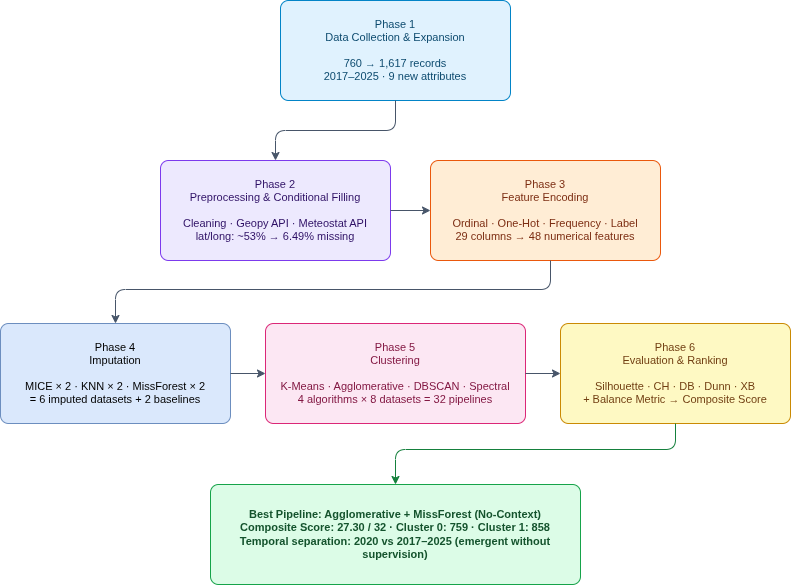
\includegraphics[width=\textwidth,height=0.75\textheight,keepaspectratio]{image21.png}
  \caption[High-level overview of the six-phase research framework]{High-level overview of the six-phase research framework adopted in this study.}
  \label{fig:methodology_framework_overview}
\end{figure}

The pipeline produces eight datasets in total --- six fully imputed and two non-imputed baselines. Each dataset is clustered by all four algorithms, giving 32 end-to-end clustering solutions that are subsequently evaluated and ranked via the composite internal-validation framework.

\section{Dataset Analysis}

\subsection{Data Collection and Expansion}

The base dataset was the Kaggle Bangladesh Suicide Dataset \cite{ref5}, originally 760 records by 27 columns covering 2020. To enhance temporal coverage and analytical richness, 857 additional recent cases were collected manually from verified national and local Bangladeshi news outlets --- Prothom Alo, The Daily Star, Jugantor, Ittefaq, and several regional newspapers and online portals --- extending coverage to 2017--2025.

To capture socio-economic and clinical dimensions absent in the original dataset, nine new attributes were introduced: \texttt{family\_members}, \texttt{position\_in\_siblings}, \texttt{marital\_status}, \texttt{duration\_of\_separation}, \texttt{profession\_description}, \texttt{workplace}, \texttt{financial\_condition}, \texttt{previous\_health\_condition}, and \texttt{previous\_suicide\_attempt}. After expansion the dataset contained 1,617 records and 36 columns; the analytical dataset used downstream contains 34 columns, after the ethical removals described next.

\subsection{Removal of Irrelevant and Sensitive Columns}

Two columns were permanently removed for ethical and analytical reasons: \texttt{full\_name} (personally identifiable) and \texttt{data\_source} (the news URL did not contribute to clustering).

\subsection{Missing Value Analysis (Pre-Imputation)}

Before any imputation, missingness was analysed per feature. As summarised in Table~\ref{tbl:missingness_groups}, features fell into four bands by missing rate.

\begin{table}[H]
\centering
\caption[Feature groupings by missing-value rate]{Feature groupings by missing-value rate}
\label{tbl:missingness_groups}
\renewcommand{\arraystretch}{1.0}
\small
\begin{tabularx}{\textwidth}{|>{\hsize=0.396\hsize\linewidth=\hsize\raggedright\arraybackslash}X|>{\hsize=0.754\hsize\linewidth=\hsize\raggedright\arraybackslash}X|>{\hsize=1.851\hsize\linewidth=\hsize\raggedright\arraybackslash}X|}
\hline
\textbf{Group} & \textbf{Missing Range} & \textbf{Key Columns} \\ \hline
1 & 77.61\% -- 96.17\% & duration\_\hspace{0pt}of\_\hspace{0pt}separation, position\_\hspace{0pt}in\_\hspace{0pt}siblings, previous\_\hspace{0pt}suicide\_\hspace{0pt}attempt, previous\_\hspace{0pt}health\_\hspace{0pt}condition, family\_\hspace{0pt}members \\ \hline
2 & 45.51\% -- 53.06\% & Weather-related variables (temp\_\hspace{0pt}min, temp\_\hspace{0pt}max), latitude, longitude, profession\_\hspace{0pt}description, financial\_\hspace{0pt}condition, etc. \\ \hline
3 & 23.93\% -- 37.90\% & workplace, marital\_\hspace{0pt}status \\ \hline
4 & 0.43\% -- 18.92\% & age, gender, method, reason, hometown, etc. \\ \hline
\end{tabularx}
\end{table}

All Group~1 variables (missing rate $>$70\%) were permanently excluded, since imputing such highly sparse features would introduce excessive uncertainty and noise \cite{ref40}.

The missingness in this dataset is unlikely to be missing-completely-at-random (MCAR). Newspaper reporting foregrounds certain details (age, gender, hometown, method) and omits more sensitive or harder-to-verify information (prior mental-health history, family-conflict context, financial condition); whether a field is reported is therefore correlated both with observable features (the type of incident and the outlet) and with unobserved characteristics (such as family willingness to disclose). The most defensible assumption is that several fields are missing-at-random (MAR) at best and missing-not-at-random (MNAR) at worst. The imputation methods used in the next sections (MICE, KNN, MissForest) all rely on a MAR-style assumption to produce calibrated estimates, which bounds the strength of any subsequent interpretation: imputed values for the most sensitive fields should be read as conditional model expectations under MAR, not as recovered ground truth, and downstream cluster-level differences in such fields should be interpreted accordingly.

\section{Detailed Preprocessing Pipeline}

\subsection{Column Standardization \& Type Correction}

The raw dataset had inconsistent naming conventions, spellings, and data types. Three corrections were applied: column names converted to snake\_case; spelling errors fixed (e.g., \texttt{maritual\_status} $\to$ \texttt{marital\_status}); and numerical values stored as strings cast to appropriate integer or float types.

\subsection{Date \& Time Standardization}

The \texttt{suicide\_date} column appeared in multiple formats (string, datetime, numeric) and the time column was categorical (morning, noon, evening, night). All dates were standardised to DD/MM/YYYY and categorical times mapped to representative hours (0--23). Five temporal features were then derived: \texttt{suicide\_day}, \texttt{suicide\_month}, \texttt{suicide\_year}, \texttt{suicide\_week}, and \texttt{suicide\_weekday}.

\subsection{Categorical Value Harmonization (Manual + Semi-automated)}

Categorical variables had extensive inconsistencies from spelling variations, synonyms, casing, and over-granular labels, with the number of unique categories ranging from 7 (gender) to 594 (hometown). A column-wise iterative cleaning process merged spelling variants and synonyms, grouped similar categories into semantically consistent classes, and simplified hometown to district-level labels to reduce sparsity and address ethical concerns. The process was repeated until no duplicate semantic categories remained; after harmonisation the highest-cardinality column (hometown) was reduced to 151 unique categories.

\subsection{Conditional Filling Using External APIs}

External data sources were integrated to reduce missingness without arbitrary imputation. The cleaned hometown field was passed to the Geopy geocoding service to fill missing latitude and longitude, reducing missingness from $\sim$53\% to 6.49\% for both. A \texttt{unix\_time} feature was then constructed from \texttt{suicide\_date} and the encoded time, reducing missingness from 52.38\% to 5\%. Weather attributes were filled via the Meteostat API keyed on \texttt{unix\_time}, latitude, and longitude, prioritising hourly data and falling back to daily aggregates when hourly were unavailable. Table~\ref{tbl:api_filling_results} reports the per-column reduction.

\begin{table}[H]
\centering
\caption[Weather-related missingness before and after API filling]{Weather-related missingness before and after conditional API filling}
\label{tbl:api_filling_results}
\renewcommand{\arraystretch}{1.0}
\small
\begin{tabularx}{\textwidth}{|>{\hsize=1.182\hsize\linewidth=\hsize\raggedright\arraybackslash}X|>{\hsize=0.891\hsize\linewidth=\hsize\raggedright\arraybackslash}X|>{\hsize=0.885\hsize\linewidth=\hsize\raggedright\arraybackslash}X|>{\hsize=1.042\hsize\linewidth=\hsize\raggedright\arraybackslash}X|}
\hline
\textbf{Column} & \textbf{Before} & \textbf{After} & \textbf{Status} \\ \hline
temp\_\hspace{0pt}min & 53.06\% & 29.87\% & Reduced \\ \hline
temp\_\hspace{0pt}max & 53.06\% & 29.56\% & Reduced \\ \hline
air\_\hspace{0pt}pressure & 53.06\% & 30.43\% & Reduced \\ \hline
air\_\hspace{0pt}humidity & 53.06\% & 53.06\% & No Change \\ \hline
wind\_\hspace{0pt}speed & 52.99\% & 30.18\% & Reduced \\ \hline
wind\_\hspace{0pt}deg & 53.06\% & 53.06\% & No Change \\ \hline
\end{tabularx}
\end{table}

Values for \texttt{air\_humidity} and \texttt{wind\_deg} did not change because the API did not return data for those columns at the required date--location combinations, and no values were filled for \texttt{feels\_like}, \texttt{clouds\_sky}, \texttt{weather\_main}, or \texttt{weather\_description} for the same reason.

\subsection{Feature Engineering \& Final Cleaning}

Three final steps were applied before encoding: long free-text columns (\texttt{profession\_description}, \texttt{reason\_description}) were dropped; \texttt{suicide\_date} and \texttt{unix\_time} were removed after feature extraction; and the final feature set contained 29 columns (13 categorical, 16 numerical).

\subsection{Encoding Strategy}

Four encoding techniques converted categorical variables into numerical representations suitable for imputation and clustering, chosen by feature characteristics.

\subsubsection{Ordinal Encoding}

Variables with intrinsic order were encoded ordinally to preserve relative ordering: \texttt{age\_group}, \texttt{financial\_condition}, \texttt{weather\_main}, and \texttt{suicide\_weekday}. Mappings were manually defined from domain knowledge to ensure semantic correctness --- for example, the age groups were encoded as \{baby=0, child=1, teen=2, young=3, adult=4, middle-aged=5, old=6\}.

\subsubsection{One-Hot Encoding}

Low-cardinality nominal variables without inherent ordering were one-hot encoded, which converts each category into a separate binary indicator without imposing a spurious ordinal relationship \cite{ref41}; this was applied to \texttt{gender}, \texttt{workplace}, and \texttt{Religion}.

\subsubsection{Frequency (Proportional) Encoding}

High-cardinality categorical variables without ordinal structure were encoded using proportional frequency encoding: \texttt{profession\_group}, \texttt{hometown}, \texttt{reason}, \texttt{method}, \texttt{weather\_description}, and \texttt{marital\_status}. Applying one-hot encoding to these features would produce a highly sparse feature space and risk the curse of dimensionality --- a problem documented across the high-cardinality encoding literature \cite{ref42}. Proportional frequency encoding was chosen as a pragmatic project-specific compromise: it handles high cardinality efficiently, preserves the relative-frequency information that may carry signal in this dataset, and is fully unsupervised, which makes it directly applicable to the downstream clustering setting where the supervised target-based alternatives advocated by \cite{ref42} are unavailable.

For a categorical feature $f$ and category $c$, the proportional frequency encoding value $\phi(c, f)$ is
\begin{equation}\label{eq:frequency_encoding}
\phi(c, f) \;=\; \frac{n_{c, f}}{N_f}
\end{equation}
where $n_{c, f}$ is the number of occurrences of category $c$ in feature $f$ and $N_f$ is the total number of non-missing observations in feature $f$. Encoded values were stored in new columns to keep the original categorical variables for interpretability and post-clustering analysis.

\subsubsection{Numerical Features}

Numerical variables were retained in their original integer or floating-point form. After frequency-encoding the ordinal categoricals and one-hot encoding the nominal ones (gender, workplace, religion), the MICE/KNN input matrix comprised 37 numerical columns; MissForest, which handles categoricals natively via label encoding, was instead supplied with a 29-column matrix. Both formats are fully numerical and ready for the respective imputation routine.

\subsubsection{Label Encoding (Special Case)}

For MissForest imputation, all columns were encoded with integer labels using scikit-learn's \texttt{LabelEncoder} to fit the tree-based estimator.

\subsubsection{Decoding Preparation}

Encoding mappings for all categorical variables were saved as JSON files for consistent post-clustering decoding, enabling interpretation, cluster profiling, and visualisation of real-world patterns.

\section{Imputation Strategies}

Missing values --- stemming from incomplete newspaper coverage --- were handled through multivariate imputation to retain sample size, reduce bias, and preserve the integrity of demographic (e.g., age, gender, profession\_group), spatiotemporal (latitude, longitude, suicide\_date), and environmental (temperature, weather\_main) features. Three established methods were selected to span distinct paradigms: parametric model-based MICE, non-parametric instance-based KNN, and ensemble tree-based MissForest. The multi-method design aligns with the consensus that no single imputation technique dominates across data types and missingness patterns.

For each method, two predictor-selection strategies were applied, giving six variants. Parameters were standardised where possible for fair comparison ($k = 5$ for KNN; MissForest iterated to the Stekhoven $\Delta_F$-stopping criterion). Implementation used scikit-learn (\texttt{KNNImputer}; a custom per-variable BayesianRidge MICE-style imputer described in \S3.4.1) plus a MissForest-equivalent built on scikit-learn random-forest estimators. Post-imputation residual missingness was $\leq$0.25\% across all variants, yielding effectively complete datasets.

\subsection{Common Functionalities of All Three Methods}

MICE, KNN, and MissForest share a common operational skeleton: a predictor-selection step that decides which columns inform the imputation, a set of value constraints that enforce feasibility of imputed values, and a generalised iterative workflow that drives the fitting.

\subsubsection{Predictor Selection Strategies}

Two strategies were used, covering both selective and inclusive scenarios.

\textbf{Correlation-based (context-aware) selection.} For each target column, pairwise Pearson correlation coefficients were computed against all other columns using pandas' \texttt{corr()}; self-correlations were excluded, and only non-zero correlations ($|r| > 0$) were retained, sorted by descending absolute value. The resulting ranking served as a heuristic predictor-selection signal rather than a formally calibrated statistical test. Many post-encoding columns are not strictly continuous --- one-hot indicators are 0/1 variables, frequency-encoded fields lie on the unit interval, and ordinal codes are integer-valued --- so Pearson correlation on them measures linear co-occurrence rather than satisfying its standard bivariate-normal assumptions. The magnitudes are therefore treated as a pragmatic ranking signal (``which columns tend to move together''), not as estimates of an underlying population correlation; only the rank, not the magnitude, drives predictor selection. The heuristic is adopted deliberately as a lightweight, transparent alternative to more sophisticated mixed-type association measures (e.g., Cram\'er's V, correlation ratio) and is recorded as a methodological design choice rather than as a rigorous statistical commitment.

\textbf{All-available (no-context) selection.} This baseline used all columns in the dataset (except the target itself) as predictors, maximising available information at the cost of potentially including weakly related or redundant variables.

\subsubsection{Constraints}

To prevent unrealistic imputed values (e.g., negative temperatures or latitudes outside Bangladesh), post-prediction constraints were applied to selected numerical, temporal, and encoded columns. Constraints came from domain knowledge, geographic facts, historical weather records, and logical limits --- examples include age (0--100 years), latitude and longitude (Bangladesh-specific geographic bounds), temperature-related columns (\texttt{feels\_like}, \texttt{temp\_min}, \texttt{temp\_max}: plausible regional range, originally specified in Kelvin), \texttt{wind\_deg} (0--360$^{\circ}$), and encoded ordinal columns (e.g., \texttt{suicide\_weekday\_encoded}: 0--6). Values were rounded for integers and clipped to bounds.

\paragraph{Note on temperature unit consistency.} The temperature constraint above was specified in Kelvin because the original Kaggle subset stored \texttt{feels\_like}, \texttt{temp\_min}, and \texttt{temp\_max} on a Kelvin scale, whereas the manually collected 2017--2025 cases were filled via Meteostat on a Celsius scale and were not converted to Kelvin before imputation. The two source cohorts therefore coexist in the same columns under different units, and the Kelvin-range constraint does not enforce a consistent physical range across the combined dataset. The inconsistency was identified after the 32-pipeline experiment had been executed, and re-running the entire pipeline was not feasible within the project timeline. The original results are retained, and the inconsistency is flagged explicitly here, in \S\ref{sec:source_cohort_caveat}, and as Limitation~\ref{lim:temp_units} in \S6.4, so that environment-related interpretations of the cluster profiles in Chapter~4 are read with appropriate caution.

\subsubsection{Functions Overview (Generalized Workflow)}

Custom Python functions processed the imputation column-by-column, taking as input the target \texttt{column\_name}, DataFrame \texttt{df}, predictor-selection dictionary (context-aware or no-context), and constraints dictionary. The common workflow was:

\begin{enumerate}[leftmargin=2em,labelindent=0pt,itemsep=0.4em]
  \item Identify rows with missing values in the target column.
  \item For each missing row, dynamically select usable predictors (non-null in that row).
  \item If no usable predictors exist, skip the row.
  \item Prepare training data from complete cases (rows where target and selected predictors are non-null).
  \item Train the appropriate model and predict the missing value (missing predictors temporarily filled with column mean for numerics or mode for categoricals).
  \item Apply rounding (for integers) and clip to constraint bounds.
  \item Update the DataFrame with the imputed value.
\end{enumerate}

This shared structure ensured consistency across methods; differences arose only from model type and encoding compatibility. Figure~\ref{fig:unified_imputation_workflow_fo} visualises the workflow, with branches for context-aware and no-context predictor selection.

\begin{figure}[!htb]
  \centering
  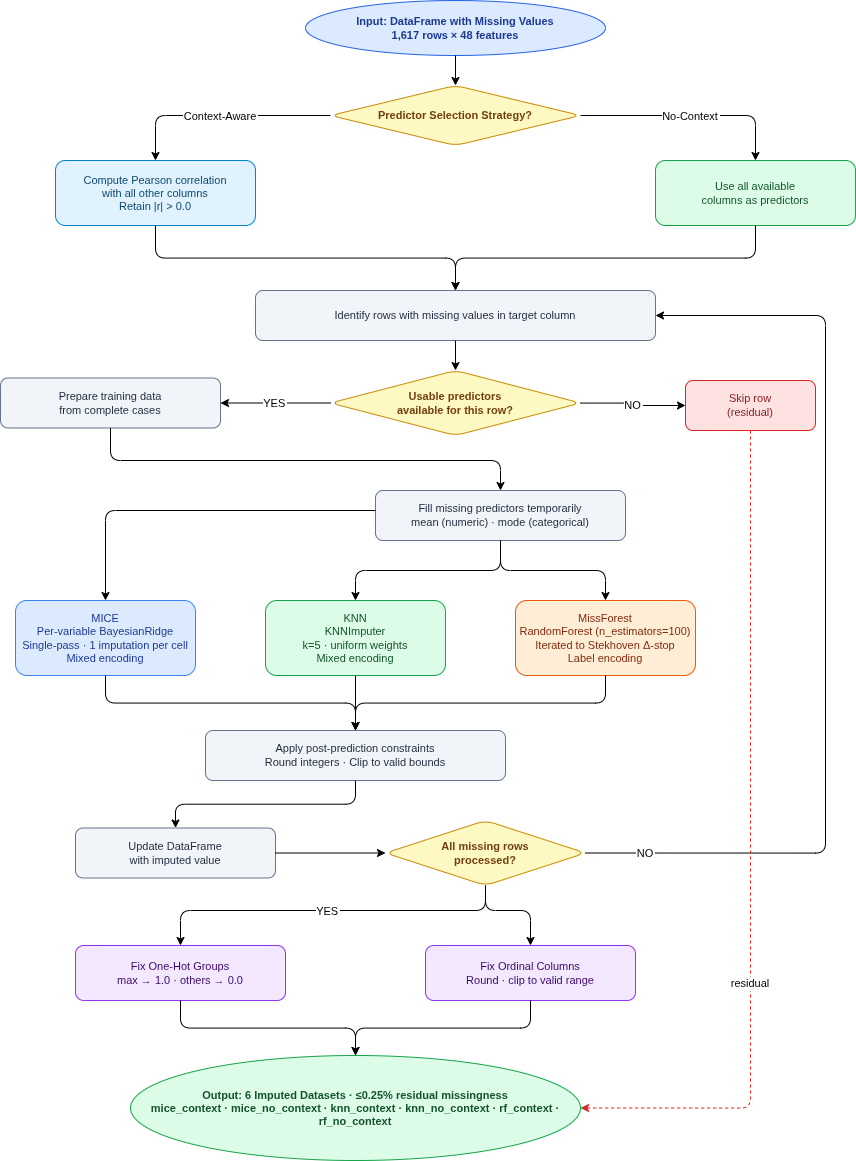
\includegraphics[width=\textwidth,height=0.9\textheight,keepaspectratio]{imputation.png}
  \caption[Unified imputation workflow for MICE, KNN, and MissForest]{Unified imputation workflow for MICE, KNN, and MissForest (context-aware vs. no-context variants).}
  \label{fig:unified_imputation_workflow_fo}
\end{figure}

\subsection{Method-Specific Adaptations}

Within the shared skeleton, each method differs in its estimator and in how it accommodates the dataset's mixed numerical and categorical columns.

\subsubsection{Multiple Imputation by Chained Equations (MICE)}

MICE is a flexible iterative method that models each variable conditionally on the others using chained regression equations \cite{ref10}; it suits mixed-type data under MAR assumptions. Rather than calling scikit-learn's \texttt{IterativeImputer} (which sweeps all columns simultaneously and produces a single imputation per cell), a custom per-variable BayesianRidge regressor was implemented to give explicit control over which predictors are used for each target column under the two predictor strategies described below. For each column with missing entries, a BayesianRidge model was fit on the rows where that column was observed, using the remaining columns (full predictor set in the no-context regime, correlation-filtered subset in the context-aware regime), and then used to predict the missing values; predictor cells that were themselves missing at prediction time were filled with the column mean. This is a single-imputation procedure: it produces one filled value per missing cell rather than the multiple imputations of Rubin's original MICE formulation, an explicit simplification motivated by the downstream clustering pipeline, which consumes a single completed matrix.

\subsubsection{K-Nearest Neighbours (KNN)}

KNN is a non-parametric instance-based method that fills missing values by averaging --- or taking the mode for categoricals --- from the $k$ most similar complete observations \cite{ref11}. The implementation used scikit-learn's \texttt{KNNImputer} ($k=5$, uniform weights) and supported mixed encodings under both predictor strategies.

\subsubsection{MissForest}

MissForest is a non-parametric iterative method that uses random forests to impute missing values, capturing non-linear interactions without distributional assumptions \cite{ref12}. It was applied with 100 trees per forest (\texttt{n\_estimators=100}) and a fixed random state for reproducibility. Label encoding was preferred for categoricals to optimise tree-based performance (unlike the mixed encoding used for MICE/KNN), and imputed categorical values were rounded and clipped to valid integer ranges post-imputation to match the original encoding.

\subsection{Post-Imputation Processing}

After imputation, two post-processing steps ensured categorical integrity, identically applied across all variants. \textit{One-hot encoded groups} (e.g., gender: female/male/third gender; workplace: rural/semi-urban/urban; religion: buddhist/christian/hindu/indigenous/muslim) sometimes produced fractional or multiple active values; these were corrected by setting the column with the highest imputed value to 1.0 and all others in the group to 0.0 per row. \textit{Ordinal columns} (e.g., \texttt{suicide\_weekday\_encoded}: 0--6; \texttt{age\_group\_encoded}: 0--6; \texttt{financial\_condition\_encoded}: 0--4; \texttt{weather\_main\_encoded}: 0--7) were rounded from floats to the nearest integers and clipped to valid bounds to restore semantic meaning.

\subsection{Summary of Imputation Variants}

Table~\ref{tbl:imputation_variants} summarises the six variants, including abbreviations (initial missingness varied by column; post-imputation $\leq$0.25\% for all variants).

\begin{table}[H]
\centering
\caption[Summary of the six imputation variants]{Summary of the six imputation variants (three methods $\times$ two predictor strategies)}
\label{tbl:imputation_variants}
\renewcommand{\arraystretch}{1.0}
\small
\begin{tabularx}{\textwidth}{|>{\hsize=0.769\hsize\linewidth=\hsize\raggedright\arraybackslash}X|>{\hsize=1.074\hsize\linewidth=\hsize\raggedright\arraybackslash}X|>{\hsize=0.857\hsize\linewidth=\hsize\raggedright\arraybackslash}X|>{\hsize=1.300\hsize\linewidth=\hsize\raggedright\arraybackslash}X|}
\hline
\textbf{Imputation Method} & \textbf{Predictor Strategy} & \textbf{Abbreviation Used} & \textbf{Notes On Implementation} \\ \hline
MICE & Correlation-based context & mice\_\hspace{0pt}context & BayesianRidge, mixed encoding \\ \hline
MICE & All available columns & mice\_\hspace{0pt}no\_\hspace{0pt}context & BayesianRidge, mixed encoding \\ \hline
KNN & Correlation-based context & knn\_\hspace{0pt}context & KNNImputer, mixed encoding \\ \hline
KNN & All available columns & knn\_\hspace{0pt}no\_\hspace{0pt}context & KNNImputer, mixed encoding \\ \hline
MissForest & Correlation-based context & rf\_\hspace{0pt}context & RandomForest, label encoding + rounding \\ \hline
MissForest & All available columns & rf\_\hspace{0pt}no\_\hspace{0pt}context & RandomForest, label encoding + rounding \\ \hline
\end{tabularx}
\end{table}

\section{Clustering Algorithms}

\subsection{Dataset Preparation for Clustering}

The clustering stage operated on 8 datasets to enable a comprehensive comparison between imputed and non-imputed versions. The 6 imputed datasets came from the three imputation methods under two predictor regimes. MICE variants retained 1{,}613 rows each (four rows whose available predictors were too sparse for a stable BayesianRidge fit were dropped), while KNN and MissForest variants kept all 1{,}617 rows. MICE and KNN variants used 37 columns (one-hot expanded categoricals) and MissForest used 29 columns (label-encoded categoricals, which the tree-based estimator can handle natively).

For baseline comparison, a non-imputed version (\texttt{df\_encoded}) was created by applying manual imputation, logical fillings, and encoding to the original data, leaving varying missingness across columns; the missing-data report showed no columns above 53.06\%, but significant missingness in groups: $>$45.51\% to $\leq$53.06\% (e.g., \texttt{feels\_like}, \texttt{air\_humidity} at 53.06\%), $>$23.93\% to $\leq$37.90\% (e.g., \texttt{workplace\_encoded} at 37.90\%), and $\leq$18.92\% (e.g., \texttt{profession\_group\_encoded} at 18.92\%).

To create complete baseline datasets, rows with any missing values were dropped and three variants formed by missingness threshold: \texttt{df\_encoded\_20} (853 rows, 22 columns, $\leq$18.92\% missing); \texttt{df\_encoded\_40} (403 rows, 30 columns, $\leq$37.90\% missing); and \texttt{df\_encoded\_50} (57 rows, 37 columns, $\leq$53.06\% missing). The 57-row \texttt{df\_encoded\_50} was excluded as too small for meaningful clustering, leaving 8 datasets in total (the 6 imputed variants plus \texttt{df\_encoded\_20} and \texttt{df\_encoded\_40}), compiled into a collection for batch processing.

\subsection{Overview and Rationale}

Clustering was applied as an unsupervised technique to discover hidden patterns in the suicide dataset, where no predefined target variable existed. The choice of clustering algorithm materially affects what structure is recovered, and clustering surveys consistently note that no single algorithm dominates when the underlying cluster geometry is unknown a priori --- spherical, elongated, density-defined, and manifold-shaped clusters each call for different inductive biases \cite{ref49}. The standard response is to run several algorithms drawn from different paradigms and let the data adjudicate. Four algorithms spanning the major paradigms were therefore selected: centroid-based (K-Means \cite{ref13}), hierarchical (Agglomerative Clustering \cite{ref14}), density-based (DBSCAN \cite{ref15}), and graph-based (Spectral Clustering \cite{ref16}). Each makes a different geometric assumption --- K-Means assumes convex centroid-shaped clusters, Agglomerative builds nested partitions through linkage merges, DBSCAN identifies dense regions and explicitly tags low-density points as noise, and Spectral relaxes convexity by embedding via the graph Laplacian. Running all four on the same data stress-tests whether any recovered pattern is an artefact of one particular assumption or a stable property of the underlying records, and these four paradigms are also the most widely used in prior unsupervised studies of suicide and mental-health profiles \cite{ref34, ref35, ref36, ref37}, which makes the clusters reported in Chapter~4 directly comparable with that literature.

Running 4 algorithms across 8 input datasets gives 32 combinations, ranked under a combined scoring system to identify the best pipeline. The design lets us assess how imputation strategy influences cluster quality while surfacing candidate demographic or environmental groupings for further exploratory analysis, subject to the limitations discussed in Chapters~4 and~6.

\subsection{Common Preprocessing and Evaluation}

All clustering methods shared a preprocessing and evaluation skeleton; parameters were tuned dynamically via grid search and fine-tuning.

\subsubsection{Preprocessing Pipeline}

Numerical columns were scaled with \texttt{StandardScaler} (mean 0, std 1) so each feature contributed equally to distance metrics, and PCA was then applied to compress dimensionality while retaining significant variance (99\% variance for K-Means; fixed component counts of 10 for Agglomerative and DBSCAN, 20 for Spectral) --- improving efficiency and reducing noise without losing key patterns.

\subsubsection{Optimal Cluster Number Determination}

The optimal number of clusters $k$ was determined via silhouette analysis (cohesion/separation) and the elbow method (inertia vs. $k$). Tested ranges varied by method (2--20 for K-Means, 2--11 for Agglomerative, 2--6 for Spectral) and were applied per dataset to adapt to varying input structures.

\subsubsection{Hyperparameter Tuning Strategy}

Hyperparameters were optimised via grid search followed by fine-tuning, with 1{,}000-row subsampling for efficiency on large datasets. Performance during tuning was assessed by silhouette (higher better), Calinski--Harabasz (higher better), and Davies--Bouldin (lower better), combined into method-specific composite scores. Parallel processing was used where applicable.

\subsection{Method-Specific Adaptations}

Each of the four algorithms shares the preprocessing and tuning skeleton above but differs in core assumptions about cluster shape, density, and connectivity.

\subsubsection{K-Means (Centroid-based)}

K-Means partitions data into $k$ clusters by minimising within-cluster variance around centroids \cite{ref13}; it is fast, scalable, and widely used but assumes spherical, equally sized clusters. It was retained as the centroid-based reference because it is the most widely used clustering method in prior unsupervised studies of suicide and mental-health profiles \cite{ref34, ref35, ref36}, making the present results directly comparable with that literature, and because it provides an inexpensive baseline against which the more flexible algorithms can be evaluated.

The implementation used dynamic hyperparameter tuning via grid search and fine-tuning. Key search spaces: $n\_\mathrm{clusters} \in [2, 20]$, init $\in \{\text{k-means++}, \text{random}\}$, $n\_\mathrm{init} \in \{10, 20, 50\}$, $\mathrm{max\_iter} \in \{300, 500\}$, with preprocessing via StandardScaler and optional PCA (99\% variance). Grid search evaluated all combinations using silhouette ($\text{sil}$, higher better) and Davies--Bouldin ($db$, lower better), selecting the best parameters via
\begin{equation}\label{eq:tuning_score_kmeans}
S_{\mathrm{KM}} \;=\; \frac{\text{sil}}{db + 10^{-12}}
\end{equation}
which favours configurations that are both internally cohesive and well separated. Fine-tuning refined $n\_\mathrm{clusters}$ around the best value ($\pm 2$, minimum 2) using \eqnref{eq:tuning_score_kmeans}, updating only if performance improved. Final labels were saved as \texttt{kmeans\_cluster}. The process was repeated independently for all 8 datasets.

\subsubsection{Agglomerative Clustering (Hierarchical)}

Agglomerative Clustering builds a hierarchy by merging the closest clusters bottom-up using linkage criteria \cite{ref14}; it handles arbitrary shapes, provides dendrograms for visualisation, and does not require a predefined cluster count. It was selected because the true number of subgroups in newspaper-reported suicide records is unknown a priori, and hierarchical merging produces a full dendrogram from which any partition level can be inspected without pre-committing to a fixed $k$; it has also been used productively in prior suicide and mental-health profiling work to recover nested sub-groupings of cases that flat partitions miss \cite{ref34, ref36}.

Implementation used dynamic hyperparameter tuning with sampling for efficiency: $n\_\mathrm{clusters} \in [2, 10]$, linkage $\in \{\text{ward}, \text{complete}, \text{average}\}$, metric $\in \{\text{euclidean}, \text{manhattan}, \text{cosine}\}$, with StandardScaler and PCA ($n\_\mathrm{components}=10$). Tuning sampled 1{,}000 rows and evaluated combinations using silhouette, Calinski--Harabasz ($ch$), and Davies--Bouldin ($db$). To combine the three indices on a common scale, $ch$ and $db$ were monotonically normalised into $[0, 1]$ as $\text{ch}_{\mathrm{n}} = ch/(ch + 10^{-6})$ and $\text{db}_{\mathrm{n}} = 1/(1 + db)$ respectively, and averaged with silhouette:
\begin{equation}\label{eq:tuning_score_three_metric}
S_{3} \;=\; \frac{\text{sil} + \text{ch}_{\mathrm{n}} + \text{db}_{\mathrm{n}}}{3}.
\end{equation}
The best parameter set maximised \eqnref{eq:tuning_score_three_metric}; final labels were saved as \texttt{agg\_cluster}. The process was repeated for all 8 datasets.

\subsubsection{DBSCAN (Density-based)}

DBSCAN groups points in high-density regions and marks low-density points as noise, identifying clusters of arbitrary shape without requiring a predefined cluster count \cite{ref15}; it is robust to outliers but sensitive to parameter choices. It was included specifically because newspaper-reported suicide data contains atypical cases (rare causes, extreme geographic or demographic combinations) alongside more common patterns: DBSCAN's explicit noise label ($-1$) sets such outliers aside rather than forcing them into the nearest cluster \cite{ref15}, avoiding a documented failure mode of centroid-based methods on heterogeneous social data \cite{ref49}.

Implementation used dynamic hyperparameter tuning with sampling: $\varepsilon \in [0.3, 2.0]$ in 0.1 increments, $\mathrm{min\_samples} \in \{3, 5, 8, 10, 15\}$, metric $\in \{\text{euclidean}, \text{manhattan}, \text{cosine}\}$, with StandardScaler and PCA ($n\_\mathrm{components}=10$). The same three-metric combined score $S_3$ from \eqnref{eq:tuning_score_three_metric} drove the search. Final labels (noise as $-1$) were saved as \texttt{dbscan\_cluster}. The process was repeated for all 8 datasets.

\subsubsection{Spectral Clustering (Graph-based)}

Spectral Clustering constructs a similarity graph and uses the eigenvalues of the graph Laplacian to partition data into non-linear clusters \cite{ref16}; it excels at capturing complex, non-convex boundaries. It was included as a deliberate complement to the centroid-based and hierarchical methods: if the true sub-groupings lie along a curved manifold rather than in compact balls --- a structure that K-Means and Ward-linkage Agglomerative cannot detect by construction --- Spectral is the algorithm best positioned to recover them \cite{ref16, ref49}.

Implementation used dynamic hyperparameter tuning with optional subsampling: $n\_\mathrm{clusters} \in [2, 6]$, affinity $\in \{\text{nearest\_neighbors}\}$, $\mathrm{assign\_labels} \in \{\text{kmeans}\}$, with StandardScaler and PCA ($n\_\mathrm{components}=20$). Combinations were evaluated using silhouette, Calinski--Harabasz, and Davies--Bouldin, combined into the Spectral-specific score
\begin{equation}\label{eq:tuning_score_spectral}
S_{\mathrm{SP}} \;=\; \text{sil} + \log\!\bigl(ch + 1\bigr) - db,
\end{equation}
in which the unbounded $ch$ is dampened logarithmically so that no single term dominates. The best parameter set maximised \eqnref{eq:tuning_score_spectral}; final labels were saved as \texttt{spc\_cluster}. The process was repeated for all 8 datasets.

\subsection{Overall Clustering Pipeline}

Each of the 8 datasets was processed uniformly: input DataFrame $\to$ standardisation $\to$ PCA dimensionality reduction $\to$ optional 1{,}000-row subsampling for tuning (the final model was always refit on the full preprocessed data) $\to$ algorithm-specific hyperparameter search with a composite score $\to$ fit of the best model and saving of the cluster-labels column (\texttt{kmeans\_cluster}, \texttt{agg\_cluster}, \texttt{dbscan\_cluster}, \texttt{spc\_cluster}). The outer loop repeated until all $8 \times 4 = 32$ pipelines were complete. Figure~\ref{fig:clustering_workflow} summarises the flow, mirroring the unified imputation workflow (Figure~\ref{fig:unified_imputation_workflow_fo}).

\begin{figure}[tp]
  \centering
  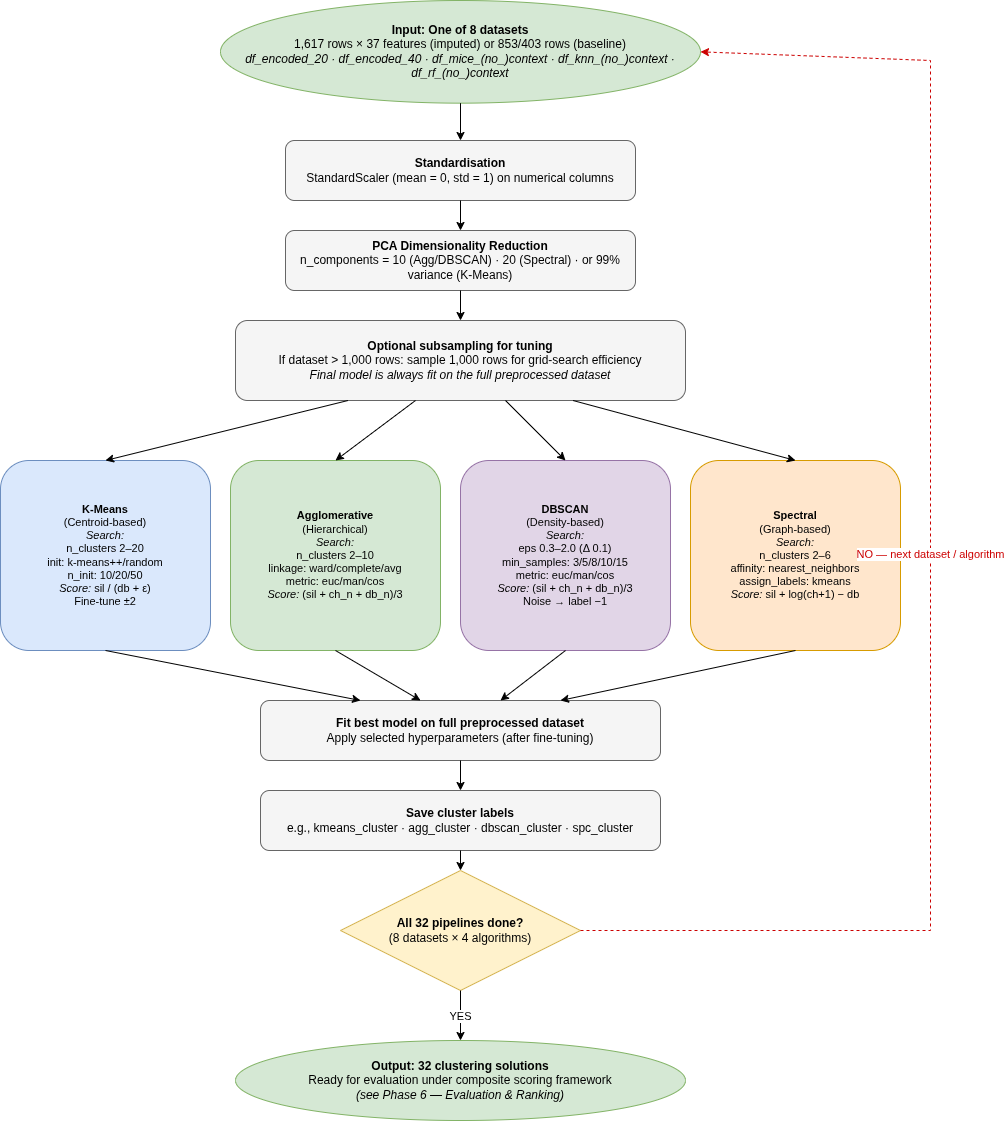
\includegraphics[width=\textwidth,height=0.85\textheight,keepaspectratio]{cluster_flow.png}
  \caption[Unified clustering workflow across the four algorithms]{Unified clustering workflow across the four algorithms (K-Means, Agglomerative, DBSCAN, Spectral). Each of the 8 input datasets is processed independently --- standardisation, PCA, an optional 1{,}000-row subsample for tuning, algorithm-specific search and composite scoring --- and the outer loop covers all 32 pipelines (8 datasets $\times$ 4 algorithms) before composite evaluation.}
  \label{fig:clustering_workflow}
\end{figure}

\subsection{Summary of Clustering Combinations}

Table~\ref{tbl:clustering_combinations_32} summarises the 32 combinations (8 inputs $\times$ 4 methods), including the abbreviation used throughout the report and the imputation method that produced each input dataset.

\begin{table}[!ht]
\centering
\caption[Summary of all 32 clustering combinations]{Summary of all 32 clustering combinations (8 input datasets $\times$ 4 algorithms)}
\label{tbl:clustering_combinations_32}
\renewcommand{\arraystretch}{1.0}
\small
\resizebox{\textwidth}{!}{%
\begin{tabular}{|l|l|l|l|}
\hline
\textbf{Input Dataset} & \textbf{Clustering Method} & \textbf{Abbreviation} & \textbf{Imputation Method} \\ \hline
df\_encoded\_20 (853 rows, 22 cols) & K-Means & kmeans\_encoded\_20 & Baseline, no imputation \\ \hline
df\_encoded\_20 & Agglomerative & agg\_encoded\_20 & Baseline, no imputation \\ \hline
df\_encoded\_20 & DBSCAN & dbscan\_encoded\_20 & Baseline, no imputation \\ \hline
df\_encoded\_20 & SPC (Spectral) & spc\_encoded\_20 & Baseline, no imputation \\ \hline
df\_encoded\_40 (403 rows, 30 cols) & K-Means & kmeans\_encoded\_40 & Baseline, no imputation \\ \hline
df\_encoded\_40 & Agglomerative & agg\_encoded\_40 & Baseline, no imputation \\ \hline
df\_encoded\_40 & DBSCAN & dbscan\_encoded\_40 & Baseline, no imputation \\ \hline
df\_encoded\_40 & SPC (Spectral) & spc\_encoded\_40 & Baseline, no imputation \\ \hline
df\_mice\_context & K-Means & kmeans\_mice\_context & Imputed with MICE \\ \hline
df\_mice\_context & Agglomerative & agg\_mice\_context & Imputed with MICE \\ \hline
df\_mice\_context & DBSCAN & dbscan\_mice\_context & Imputed with MICE \\ \hline
df\_mice\_context & SPC (Spectral) & spc\_mice\_context & Imputed with MICE \\ \hline
df\_mice\_no\_context & K-Means & kmeans\_mice\_no\_context & Imputed with MICE \\ \hline
df\_mice\_no\_context & Agglomerative & agg\_mice\_no\_context & Imputed with MICE \\ \hline
df\_mice\_no\_context & DBSCAN & dbscan\_mice\_no\_context & Imputed with MICE \\ \hline
df\_mice\_no\_context & SPC (Spectral) & spc\_mice\_no\_context & Imputed with MICE \\ \hline
df\_knn\_context & K-Means & kmeans\_knn\_context & Imputed with KNN \\ \hline
df\_knn\_context & Agglomerative & agg\_knn\_context & Imputed with KNN \\ \hline
df\_knn\_context & DBSCAN & dbscan\_knn\_context & Imputed with KNN \\ \hline
df\_knn\_context & SPC (Spectral) & spc\_knn\_context & Imputed with KNN \\ \hline
df\_knn\_no\_context & K-Means & kmeans\_knn\_no\_context & Imputed with KNN \\ \hline
df\_knn\_no\_context & Agglomerative & agg\_knn\_no\_context & Imputed with KNN \\ \hline
df\_knn\_no\_context & DBSCAN & dbscan\_knn\_no\_context & Imputed with KNN \\ \hline
df\_knn\_no\_context & SPC (Spectral) & spc\_knn\_no\_context & Imputed with KNN \\ \hline
df\_rf\_context & K-Means & kmeans\_rf\_context & Imputed with MissForest \\ \hline
df\_rf\_context & Agglomerative & agg\_rf\_context & Imputed with MissForest \\ \hline
df\_rf\_context & DBSCAN & dbscan\_rf\_context & Imputed with MissForest \\ \hline
df\_rf\_context & SPC (Spectral) & spc\_rf\_context & Imputed with MissForest \\ \hline
df\_rf\_no\_context & K-Means & kmeans\_rf\_no\_context & Imputed with MissForest \\ \hline
df\_rf\_no\_context & Agglomerative & agg\_rf\_no\_context & Imputed with MissForest \\ \hline
df\_rf\_no\_context & DBSCAN & dbscan\_rf\_no\_context & Imputed with MissForest \\ \hline
df\_rf\_no\_context & SPC (Spectral) & spc\_rf\_no\_context & Imputed with MissForest \\ \hline
\end{tabular}
}
\end{table}

\subsection{Computational Considerations}\label{sec:computational_considerations}

The 32-pipeline grid combines methods whose computational cost differs by several orders of magnitude. This subsection documents the standard asymptotic complexity of each component to explain why some combinations were practical to grid-search aggressively while others were tuning-bound. Textbook complexities are reported; per-pipeline wall-clock measurement was not instrumented in the study, and this is acknowledged openly rather than substituted with estimated runtimes.

Let $n$ denote the number of records ($n = 1{,}617$ for MissForest and KNN variants, $n = 1{,}613$ for MICE variants, $n \in \{403, 853\}$ for the encoded baselines), $p$ the number of features after encoding ($p = 37$ for MICE/KNN, $p = 29$ for MissForest), $k$ the number of clusters, $T$ the number of trees in MissForest (100), and $I$ the number of inner iterations (set to 1 in the custom MICE implementation; MissForest is iterated until the Stekhoven $\Delta_F$-stopping criterion ceases to decrease).

\textbf{Imputation methods.} The custom MICE-style imputer (per-variable BayesianRidge) is approximately $O(p \cdot n p^2)$ for the single pass, dominated by the per-variable regression fits; with $p = 37$ this is the cheapest of the three in practice. KNN imputation (\texttt{KNNImputer}, $k=5$) is $O(n^2 p)$ for the pairwise distance computation, which dominates runtime at $n = 1{,}617$. MissForest fits a separate random forest per partially observed variable per iteration, giving an approximate $O(I \cdot p \cdot T \cdot n p \log n)$ cost; with $T = 100$ trees and $p = 29$ variables iterated until convergence, it is the dominant runtime cost in the imputation stage --- already noted in \S5.5 and \S5.6, and the reason imputation hyperparameters were not swept.

\textbf{Clustering algorithms.} For each input dataset, the cost of fitting one configuration is: K-Means $O(n k d I_{\mathrm{km}})$, where $d$ is the post-PCA dimensionality and $I_{\mathrm{km}}$ the number of Lloyd iterations --- the cheapest of the four, with the dominant cost in the grid search over $k \in [2, 20]$, init methods, $n\_\mathrm{init}$, and $\mathrm{max\_iter}$ (\S3.5.3). Agglomerative Clustering: $O(n^2 \log n)$ time and $O(n^2)$ memory for the pairwise linkage matrix; at $n \approx 1{,}600$ this is comfortable within Colab free-tier RAM but binding above $n \approx 20{,}000$. DBSCAN: $O(n \log n)$ with a KD-tree neighbour query in low to moderate dimensionality (the scikit-learn default), degrading to $O(n^2)$ when the metric or dimensionality forces a brute-force neighbour search. Spectral Clustering: $O(n^3)$ for the eigendecomposition of the affinity matrix, plus $O(n^2)$ memory --- the most expensive of the four, the principal reason Spectral was not grid-searched as aggressively as K-Means, and tractable on Colab at $n \approx 1{,}600$ but binding above $n \approx 5{,}000$ on free-tier hardware.

The MissForest variants and the Spectral Clustering runs jointly account for most of the wall-clock cost of the 32-pipeline grid; these costs are the reason imputation hyperparameters were not searched and Spectral was not tuned with the same density as K-Means. The smaller baseline datasets ($n \in \{403, 853\}$) were inexpensive enough to be grid-searched freely. Per-pipeline runtimes were not recorded in the implementation; recording them is recommended for any subsequent replication that wishes to report compute budgets quantitatively (see \S6.5, Future Work).

\section{Evaluation Metrics and Combined Score Ranking}\label{sec:evaluation_metrics_combined}

\subsection{Overview of Evaluation Approach}

To compare the quality of the 32 clustering combinations consistently, a project-specific evaluation framework was developed. No single index fully captures clustering quality, since different indices emphasise different aspects --- cohesion, separation, compactness --- so five established internal validation metrics were selected and supplemented by an additional balance penalty term designed to demote configurations that achieve high geometric scores while producing near-degenerate cluster assignments (one mega-cluster plus singletons, or DBSCAN solutions in which the bulk of points are flagged as noise). The balance term is a pragmatic, study-specific scoring component, not a proposed general-purpose clustering metric. The framework aggregates these metrics into a composite ranking score, penalising cases with high geometric quality but poor interpretability, and was applied uniformly to all 32 cases with NaNs handled gracefully.

\subsection{Standard Clustering Validation Metrics}

Five widely used metrics were employed to evaluate geometric and structural aspects of the clusters. Each was computed for the full dataset (excluding noise labels of $-1$ in DBSCAN cases, where a mask focused the computation on clustered points).

\paragraph{Silhouette Score \cite{ref17}.} Measures how similar a point is to its own cluster compared to other clusters, ranging from $-1$ (poor) to $1$ (excellent):
\begin{equation}\label{eq:silhouette}
s(i) \;=\; \frac{b(i) - a(i)}{\max\bigl(a(i),\, b(i)\bigr)}
\end{equation}
where $a(i)$ is the average distance from $i$ to other points in its cluster and $b(i)$ is the minimum average distance from $i$ to points in another cluster. The overall score is the mean $s(i)$ across all points; higher is better.

\paragraph{Calinski--Harabasz Index (Variance Ratio Criterion) \cite{ref18}.} The ratio of between-cluster to within-cluster dispersion:
\begin{equation}\label{eq:calinski_harabasz}
CH \;=\; \frac{B/(K-1)}{W/(n-K)}
\end{equation}
where $B$ is the between-cluster sum of squares, $W$ the within-cluster sum, $K$ the number of clusters, and $n$ the number of points. Higher indicates compact, well-separated clusters.

\paragraph{Davies--Bouldin Index \cite{ref19}.} The average similarity between each cluster and its most similar neighbour:
\begin{equation}\label{eq:davies_bouldin}
DB \;=\; \frac{1}{K} \sum_{i=1}^{K} \max_{j \neq i} \left( \frac{s_i + s_j}{d_{ij}} \right)
\end{equation}
where $s_i$ is the average intra-cluster distance in cluster $i$ and $d_{ij}$ the distance between centroids of $i$ and $j$. Lower is better; in code it was inverted as $db_{\mathrm{inv}} = 1/(1 + db)$ to align with higher-better composites.

\paragraph{Dunn Index \cite{ref20}.} Compactness (maximum intra-cluster distance) against separation (minimum inter-cluster distance):
\begin{equation}\label{eq:dunn}
D \;=\; \frac{\min_{i \neq j} d(c_i, c_j)}{\max_{k} \delta(c_k)}
\end{equation}
where $d(c_i, c_j)$ is the minimum distance between points in clusters $i$ and $j$ and $\delta(c_k)$ the maximum within $k$. Higher is better.

\paragraph{Xie--Beni Index \cite{ref21}.} Compactness relative to separation, originally formulated for fuzzy partitioning; the crisp form is used here:
\begin{equation}\label{eq:xie_beni}
XB \;=\; \frac{\displaystyle \sum_{k=1}^{K} \sum_{x_i \in C_k} \|x_i - c_k\|^2}{\displaystyle n \cdot \min_{i \neq j} \|c_i - c_j\|^2}
\end{equation}
where $C_k$ is the set of points assigned to cluster $k$ and $c_k$ are centroids. Lower is better; inverted as $xb_{\mathrm{inv}} = 1/(1 + xb)$ for higher-better composites.

These metrics were chosen for their complementary strengths in assessing geometric validity, though they do not penalise size imbalance or excessive noise --- the gap that the next subsection addresses.

\subsection{Study-Specific Balance Penalty Term}

Standard internal validation metrics do not penalise cluster-size imbalance, so they assign high scores to configurations that are geometrically tight but structurally near-degenerate (one large cluster and many singletons, or DBSCAN solutions in which 99\% of points are labelled noise). To prevent such configurations from dominating the ranking, a balance penalty term was added; it rewards reasonably even point distribution and penalises over-segmentation and high noise rates. This is a study-specific scoring choice tailored to the imbalances commonly encountered in newspaper-derived social data, not a proposed general-purpose clustering metric.

Let $L$ be the array of cluster labels (excluding noise/$-1$ for DBSCAN), $K$ the number of unique clusters ($\geq 2$, else score $= 0$), $c_k$ the size of cluster $k$, $n = \sum c_k$, and $p_k = c_k / n$ the proportions. The base balance (evenness) is
\begin{equation}\label{eq:balance_base}
\text{base} \;=\; 1 \;-\; \sqrt{\frac{1}{K} \sum_{k=1}^{K} \left( p_k - \frac{1}{K} \right)^{\!2}}
\end{equation}
which is 1 for perfectly equal sizes and decreases with imbalance. The full balance term applies a $1/\sqrt{K}$ penalty for excessive cluster counts:
\begin{equation}\label{eq:balance}
\text{balance} \;=\; \text{base} \,\times\, \frac{1}{\sqrt{K}}
\end{equation}
The result ranges roughly 0--1, with higher values for balanced, moderately segmented clusters. In practice, the balance term prevents imbalanced clusters from absorbing rare or smaller subgroups (specific professions, hometowns) into a dominant mega-cluster or labelling them as noise, which would weaken any subsequent profiling. The term complements rather than replaces the standard geometric indices and is offered as a project-specific composite-scoring choice for highly imbalanced, noise-prone social datasets, not as a general-purpose contribution to clustering theory.

\subsection{Composite Scoring and Ranking Framework}

To integrate the six metrics into a single ranking, a weighted rank-based aggregation was used. The approach handles differing scales, directions (higher/lower better), and NaN cases, while prioritising interpretability through a high weight on the balance metric.

For each of the 32 cases, metrics were computed and ranked descending per metric (higher-better for silhouette, Calinski--Harabasz, Dunn, balance, and the inverted Davies--Bouldin/Xie--Beni; NaNs ranked last). Points were assigned as $n - r$, where $n = 32$ and $r$ is the rank position (top $=$ 0; NaN $= 0$ points). The composite score for a case was
\begin{equation}\label{eq:composite_score}
\text{score} \;=\; \sum_{m=1}^{6} \omega_m \times (n - r_m)
\end{equation}
where $\omega_m$ is the weight of metric $m$ and $r_m \in \{0, 1, \ldots, n-1\}$ its zero-indexed rank (best $= 0$); NaN values contribute 0 points directly, bypassing \eqnref{eq:composite_score}. Cases were sorted by descending score for the final ranking.

Weights were selected empirically. Several combinations were tested, and the resulting top-ranked clusters were manually inspected for interpretability, noise levels, size balance, and logical distinguishability. The final weights (Table~\ref{tbl:weights_for_composite_score}) produced the most meaningful, well-distributed, low-noise clusters for exploratory subgroup analysis.

\begin{table}[H]
\centering
\caption[Weights for composite score]{Weights for composite score}
\label{tbl:weights_for_composite_score}
\renewcommand{\arraystretch}{1.0}
\small
\begin{tabularx}{\textwidth}{|>{\hsize=0.877\hsize\linewidth=\hsize\raggedright\arraybackslash}X|>{\hsize=0.547\hsize\linewidth=\hsize\raggedright\arraybackslash}X|>{\hsize=1.576\hsize\linewidth=\hsize\raggedright\arraybackslash}X|}
\hline
\textbf{Metric} & \textbf{Weight} & \textbf{Rationale} \\ \hline
balance & 0.35 & Highest priority for size equity and noise control \\ \hline
silhouette & 0.25 & Core measure of cohesion/separation \\ \hline
calinski\_\hspace{0pt}harabasz & 0.20 & Strong variance-based separation indicator \\ \hline
dunn & 0.10 & Distance-based compactness/separation \\ \hline
davies\_\hspace{0pt}bouldin & 0.05 & Cluster similarity (inverted) \\ \hline
xie\_\hspace{0pt}beni & 0.05 & Compactness relative to separation (inverted) \\ \hline
\end{tabularx}
\end{table}

Because all 32 cases are ranked, the highest achievable composite score is 32 and the lowest is 1; cases closer to 32 perform better.

\subsection{Group-Level Comparisons}

To compare across imputation strategies, predefined groups were formed: \texttt{no\_context\_dfs} (all no-context imputed), \texttt{context\_dfs} (all context-aware imputed), \texttt{no\_imputed\_dfs} (baseline encoded), \texttt{mice\_dfs}, \texttt{rf\_dfs}, \texttt{knn\_dfs}, and algorithm-specific groups (\texttt{agg\_dfs}, \texttt{dbscan\_dfs}, \texttt{kmeans\_dfs}, \texttt{spc\_dfs}). Group averages were computed per metric, with NaNs skipped, for visualisation and cross-analysis. Metrics were normalised via min--max scaling (per metric across all cases) for comparative graphing.

\subsection{Additional Analysis for Best Cases}

After ranking, top cases were selected for decoding and profiling. Label-encoded features were decoded using the saved JSON files from preprocessing, mapping integers back to original categories for cluster interpretation, visualisation, and exploratory subgroup characterisation.

\section{Summary of the Complete Pipeline}

The methodology described in this chapter assembles raw newspaper records into a clean, encoded analytical dataset; produces six imputed variants from three methods under two predictor regimes; runs four clustering algorithms across the resulting eight inputs; and ranks the 32 end-to-end pipelines under a balance-aware composite score. Figure~\ref{fig:complete_pipeline_integration} consolidates the six phases into a single integrated view.

\begin{figure}[!htb]
  \centering
  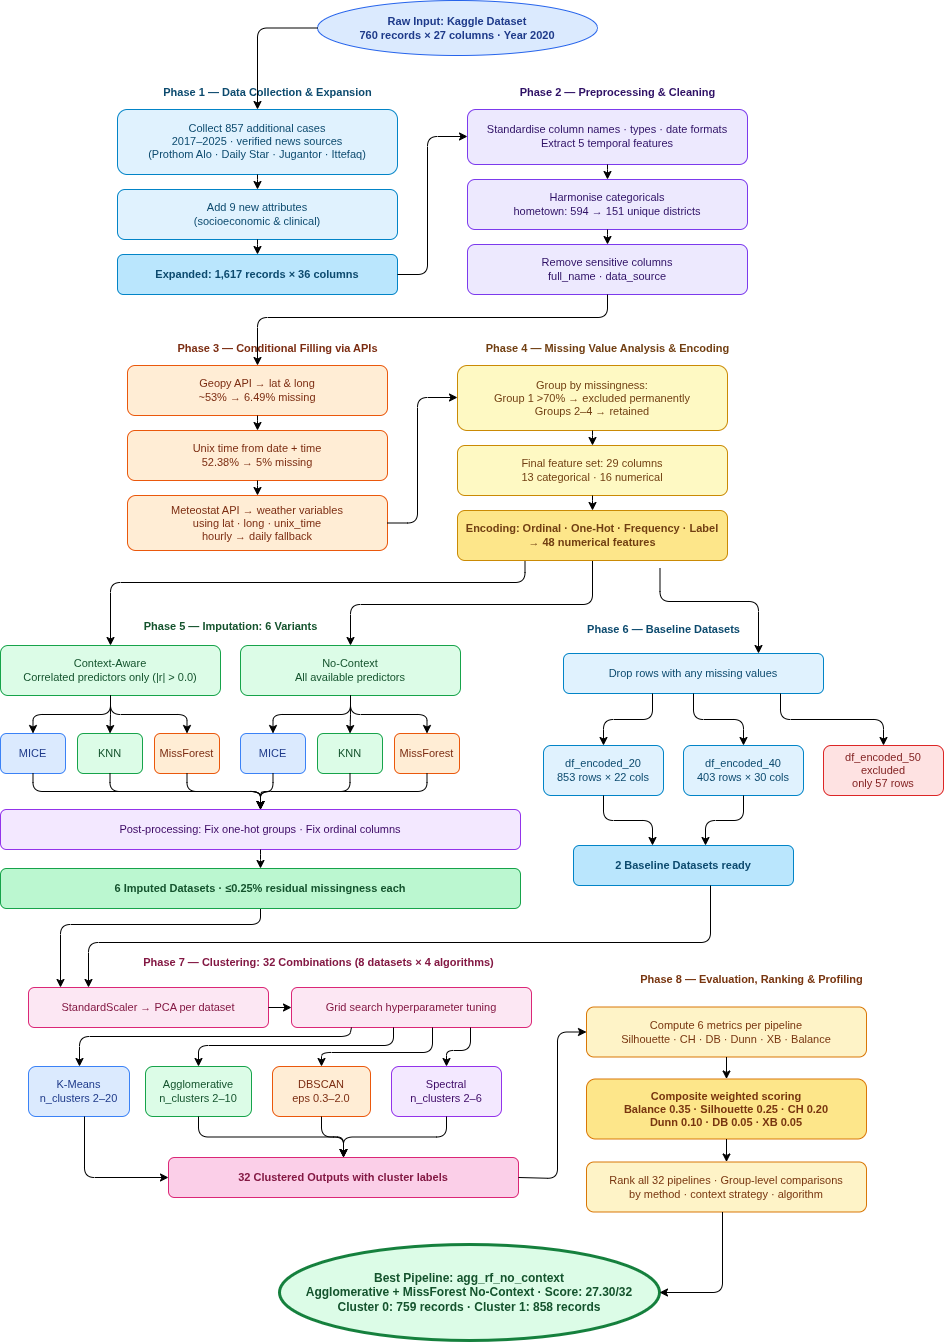
\includegraphics[width=\textwidth,height=0.9\textheight,keepaspectratio]{overall.png}
  \caption[Integrated view of the complete pipeline]{Integrated view of the complete pipeline, showing how all six phases combine to produce the 32 end-to-end clustering combinations evaluated in Chapter~4.}
  \label{fig:complete_pipeline_integration}
\end{figure}

% Chapter 4: Implementation and Result Analysis
\chapter{Implementation and Result Analysis}

\section{Implementation Overview}

The pipeline described in Chapter~3 was implemented in Python and organised into four modular stages mirroring the methodology phases: preprocessing, imputation, clustering, and evaluation. Each stage ran in Google Colab and persisted its output as a serialised dataset, so any stage could be re-run independently without recomputing upstream work. The preprocessing stage performed cleaning, conditional API-based filling of geolocation and weather, categorical harmonisation, feature engineering, and the multi-strategy encoding detailed in Section~3.3. The imputation stage produced the six imputed datasets: MICE variants retained 1{,}613 rows $\times$ 37 columns after dropping four rows whose available predictors were too sparse for stable BayesianRidge fitting; KNN variants retained the full 1{,}617 rows $\times$ 37 columns; and MissForest variants retained 1{,}617 rows $\times$ 29 columns (the tree-based estimator uses label-encoded categoricals rather than the one-hot expansion used for MICE/KNN). The full per-variant accounting is given in \S3.4.2. The clustering stage applied K-Means, Agglomerative, DBSCAN, and Spectral Clustering to each of the eight input datasets --- the six imputed variants and the two non-imputed baselines, \texttt{df\_encoded\_20} (853 rows, 22 columns) and \texttt{df\_encoded\_40} (403 rows, 30 columns). The evaluation stage computed the six internal-validation metrics, the balance penalty term, and the composite ranking score of \S\ref{sec:evaluation_metrics_combined}.

Inside the clustering stage, each input dataset was processed through StandardScaler and optional PCA (99\% variance for K-Means, 10 components for Agglomerative and DBSCAN, and 20 for Spectral), with the algorithm-specific composite tuning scores defined in \eqnref{eq:tuning_score_kmeans}--\eqnref{eq:tuning_score_spectral}. Optimal cluster labels were appended to the original DataFrames as \texttt{kmeans\_cluster}, \texttt{agg\_cluster}, \texttt{dbscan\_cluster}, and \texttt{spc\_cluster}. Datasets were organised into logical groups for cross-strategy analysis (algorithm-specific: \texttt{agg\_dfs}, \texttt{dbscan\_dfs}, \texttt{kmeans\_dfs}, \texttt{spc\_dfs}; imputation-specific: \texttt{context\_dfs}, \texttt{no\_context\_dfs}, \texttt{no\_imputed\_dfs}, \texttt{mice\_dfs}, \texttt{rf\_dfs}, \texttt{knn\_dfs}), and the same grouping is reused in \S\ref{sec:group_level_analysis}. Key libraries were scikit-learn (preprocessing, clustering, internal validation), NumPy and SciPy (distance computations for the Dunn and Xie--Beni indices), pandas (dataset manipulation), and matplotlib/seaborn (visualisation).

\textbf{Reproducibility.} The 12-notebook pipeline ran in Google Colab on the platform's default runtime during the 2024--2025 project period (Python 3.10/3.11, scikit-learn 1.3 or later, NumPy 1.x, pandas 2.x, SciPy 1.x). All stochastic components were initialised with a fixed seed (\texttt{random\_state=42}) applied uniformly across MissForest (100 trees), the custom per-variable BayesianRidge MICE-style imputer described in \S3.4.1, the K-Means grid search ($n\_\mathrm{clusters} \in [2, 20]$, init $\in \{\text{k-means++}, \text{random}\}$, $n\_\mathrm{init} \in \{10, 20, 50\}$, $\mathrm{max\_iter} \in \{300, 500\}$), the Spectral Clustering eigendecomposition, and the train/validation splits used in imputation diagnostics. The KNN imputer was configured with $k = 5$ and Euclidean distance. The clustering-stage PCA retained 99\% of variance for K-Means, 10 components for Agglomerative and DBSCAN, and 20 for Spectral. Intermediate datasets are persisted as Excel files after every stage (\texttt{0\_original.xlsx} through \texttt{11\_forest\_no\_context.xlsx}, plus per-algorithm clustering outputs in \texttt{datasets/\{agg, kmeans, dbscan, spc\}/}). Data availability and the public code release are described in \S\ref{sec:data_availability}.

\section{Cluster Quality Comparison}

\subsection{Initial Manual Evaluation}

Initial inspection of the 32 outputs revealed substantial variation in quality. Some DBSCAN configurations posted high silhouette scores (e.g., 0.8744) while forming only tiny clusters --- two of 3 points each, with 1{,}611 of 1{,}617 points labelled as noise. The pattern is a known failure mode of standard geometric indices, which can reward small compact clusters while ignoring excessive noise and poor data utilisation, and similar issues appeared across algorithms (a dominant cluster with many singletons). These observations motivated the inclusion of the study-specific balance penalty inside the composite score, to discourage degenerate partitions and to keep ranking decisions aligned with interpretable, well-utilised clusters.

\subsection{Composite Scoring and Ranking}

The 32 clustering combinations were ranked using the composite framework of \S\ref{sec:evaluation_metrics_combined} (\eqnref{eq:composite_score}). Figure~\ref{fig:composite_scoring_and_ranking} presents a heatmap of normalised metric values (min--max scaling per metric) and composite scores, sorted by final rank --- higher values redder, lower bluer. Raw (non-normalised) metric values for all 32 cases appear in the Annex (Table~\ref{tbl:full_per_case_results_across_a}).

The ranking shows clear patterns. Imputed datasets dominate the top positions: all top 10 cases are imputed (6 no-context, 4 context-aware), consistent with the expectation that principled imputation improves downstream clustering quality. Among imputed cases, no-context variants hold a small lead over context-aware ones, occupying 6 of the top 10 spots --- consistent with, though not on its own establishing, the interpretation that a larger predictor pool during imputation provides a modest, consistent benefit on this dataset. Within the imputed pipelines, MissForest configurations occupy 6 of the top 10 (with 2 each from MICE and KNN); on the metrics used in this study and for this dataset, MissForest is therefore the strongest imputation backbone of the three, framed as a dataset-specific observation rather than a general superiority claim, since imputation method rankings are well known to vary with sample size, missingness mechanism, and feature types.

Algorithm diversity is also visible. Spectral Clustering (\texttt{spc}) leads with 5 cases in the top 10, followed by Agglomerative and K-Means. The single best combination is Agglomerative Clustering with MissForest no-context imputation (\texttt{agg\_rf\_no\_context}, rank 1, composite score 27.30 out of a maximum of 32). High-noise or severely imbalanced cases (notably DBSCAN with tiny clusters) consistently rank at the bottom, confirming that the balance penalty does the work it was introduced for; the worst pipeline was DBSCAN with KNN imputation under the context-aware strategy, scoring 4.20 --- close to the theoretical minimum of 1. The metric- and group-level patterns behind these results are unpacked in the group-level comparisons (\S\ref{sec:group_level_analysis}) and the Discussion (\S\ref{sec:discussion_of_findings}).

\begin{figure}[!htb]
  \centering
  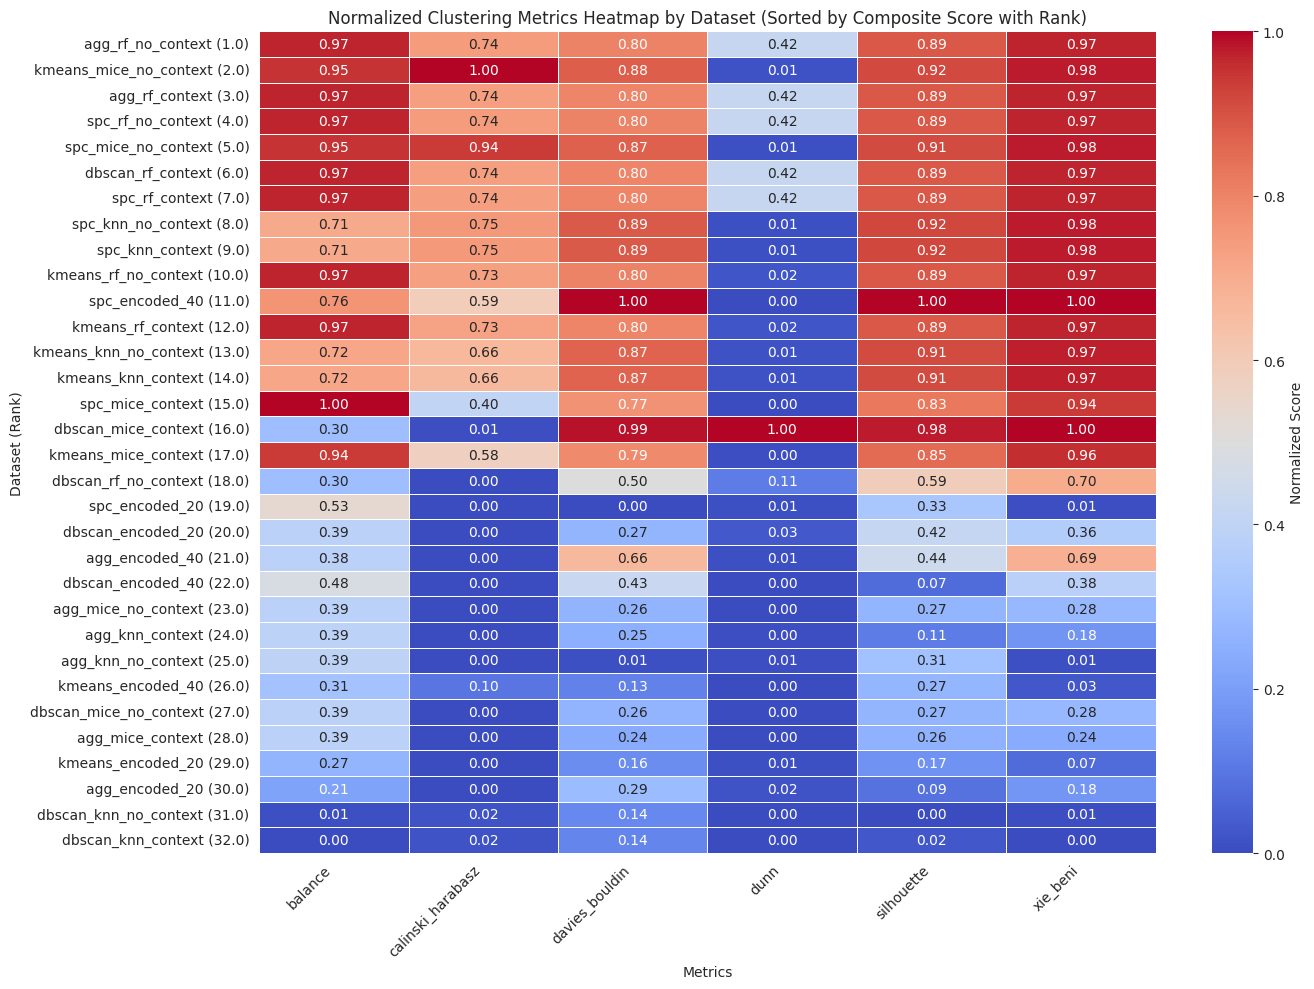
\includegraphics[width=\textwidth,height=0.55\textheight,keepaspectratio]{image22.png}
  \caption[Composite scoring and ranking heatmap]{Composite scoring and ranking heatmap. Rows sorted by final rank; columns: balance, silhouette, Calinski--Harabasz, Dunn, Davies--Bouldin (inverted), Xie--Beni (inverted), composite score. Green = higher values, red = lower values.}
  \label{fig:composite_scoring_and_ranking}
\end{figure}

\subsection{Visual Comparison of Combined Scores}

Across all 32 combinations, imputed pipelines consistently outperformed the non-imputed baselines, underscoring the improvement in clustering quality achieved through imputation. Figure~\ref{fig:horizontal_bar_graph_of_compos} visualises the ranking as a horizontal bar graph of composite scores, sorted from highest to lowest. Within the top 16, the upper-ranked solutions exhibit clear, well-separated clusters with minimal overlap, while the lower-ranked solutions display increasingly messy, heavily overlapping clusters, often with fragmentation or poor separation. Figure~\ref{fig:grid_of_pca_reduced_scatter_pl} shows PCA-reduced scatter plots for the top 16 cases as a $4 \times 4$ grid sorted by descending composite rank (top-left = best), with each subplot's points coloured by assigned cluster label; full scatter plots for all 32 cases appear in the Annex (Figure~\ref{fig:supplementary_figure_s2_full_p}).

Top-performing cases predominantly form 2 balanced clusters, reflecting interpretable, well-distributed partitioning, whereas lower-ranked cases in the top 16 tend to produce either too few clusters (excessive noise) or too many (over-segmentation), both of which correlate with reduced composite scores. Figure~\ref{fig:horizontal_bar_graph_showing_t} reports unique-cluster counts (excluding DBSCAN noise labels of $-1$) as a bar graph for the top 16 cases; full counts for all 32 cases are in the Annex (Figure~\ref{fig:supplementary_figure_s3_full_b}). The composite scoring formulation thus favours configurations with balanced, well-utilised clusters and demotes those exhibiting geometric artefacts or near-degenerate distributions, consistent with its design intent.

\begin{figure}[!htb]
  \centering
  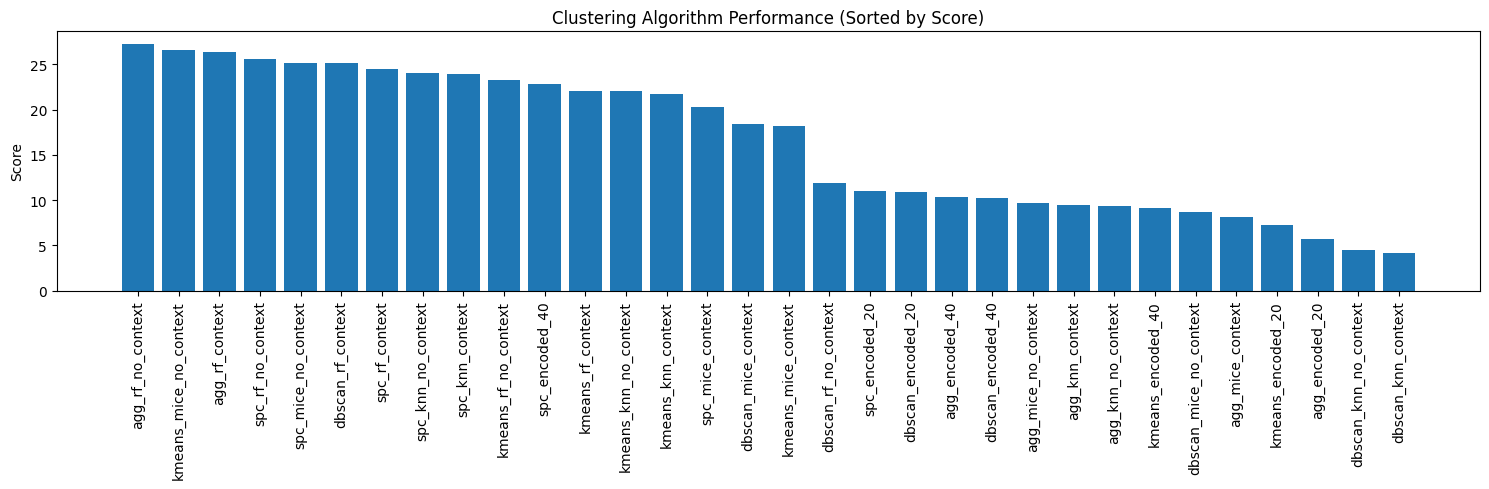
\includegraphics[width=\textwidth,height=0.5\textheight,keepaspectratio]{image7.png}
  \caption[Composite scores for all 32 clustering combinations]{Horizontal bar graph of composite scores for all 32 clustering combinations, sorted by final rank (highest to lowest).}
  \label{fig:horizontal_bar_graph_of_compos}
\end{figure}

\begin{figure}[!htb]
  \centering
  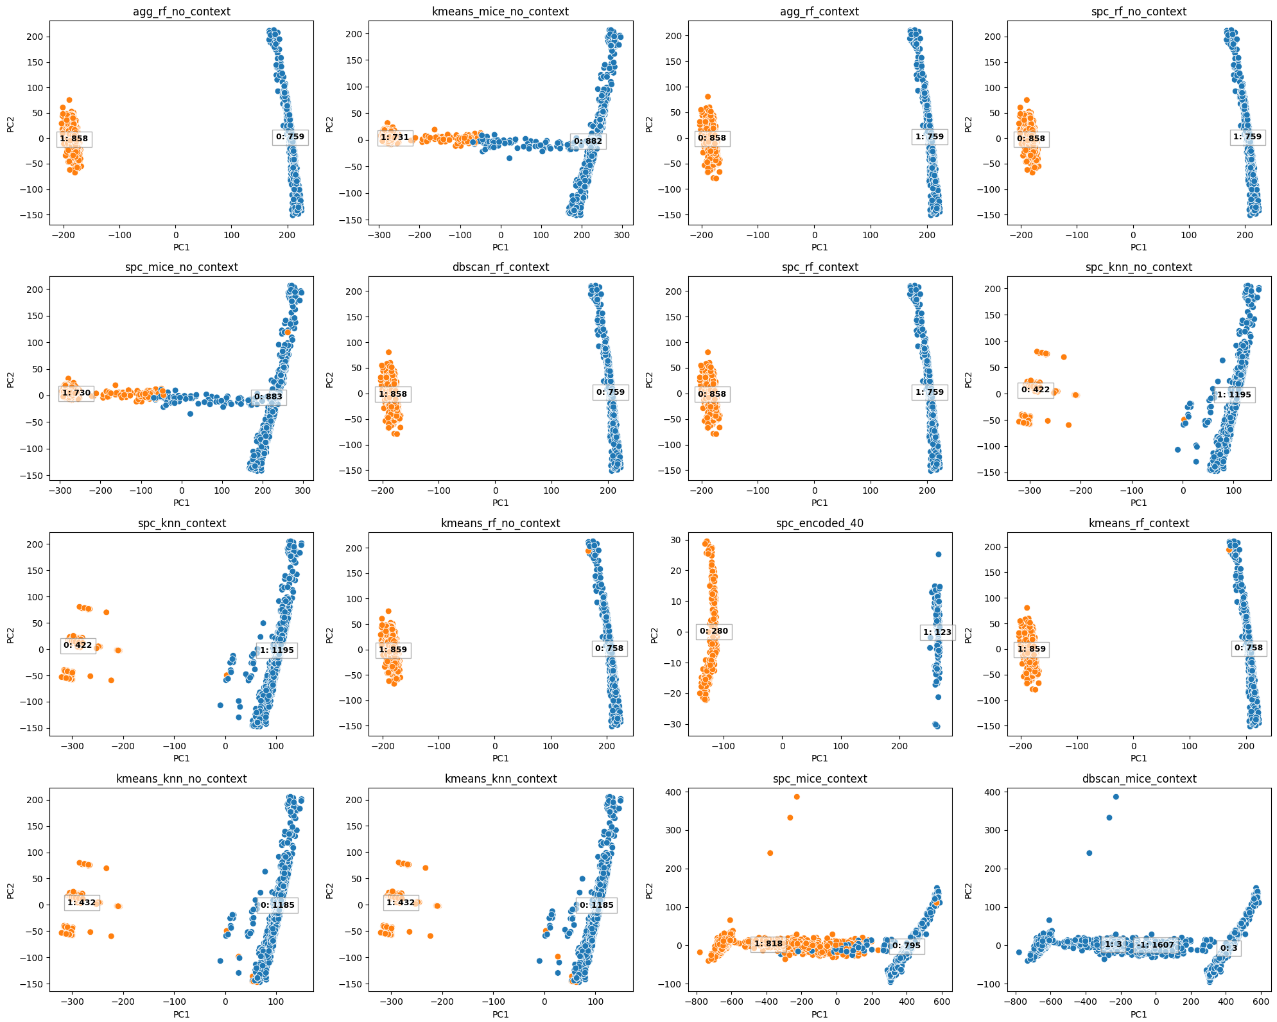
\includegraphics[width=\textwidth,height=0.8\textheight,keepaspectratio]{image14_a.png}
  \caption[PCA scatter grid for top 16 ranked cases]{Grid of PCA-reduced scatter plots (4 rows $\times$ 4 columns) for the top 16 ranked cases, sorted by descending composite rank (top-left = best). Points are coloured by cluster labels.}
  \label{fig:grid_of_pca_reduced_scatter_pl}
\end{figure}

\begin{figure}[!htb]
  \centering
  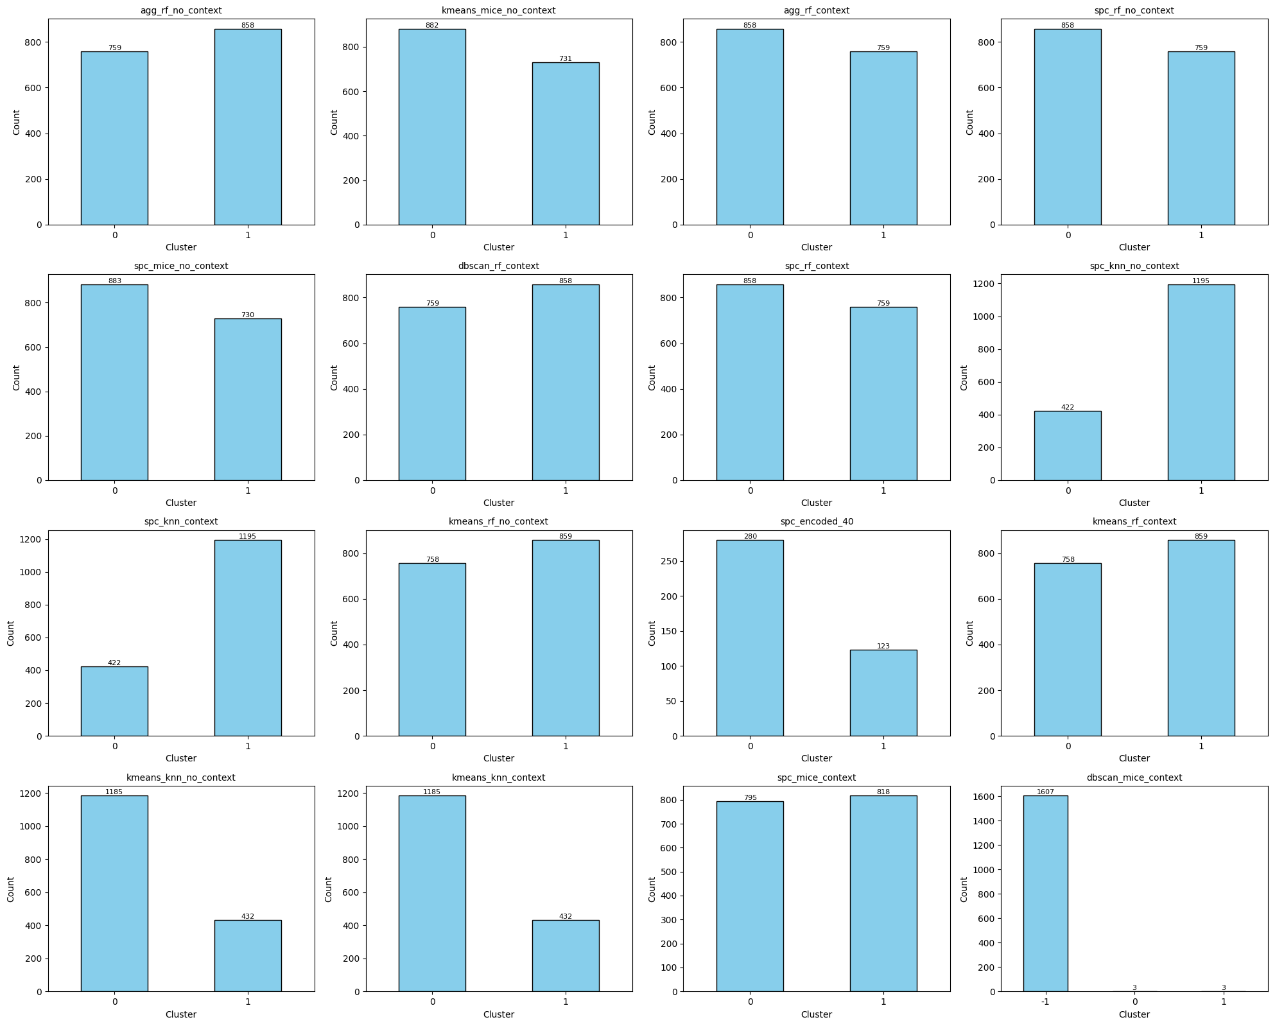
\includegraphics[width=\textwidth,height=0.8\textheight,keepaspectratio]{image8_a.png}
  \caption[Cluster count distribution for top 16 cases]{Horizontal bar graph showing the number of unique clusters (excluding noise in DBSCAN) for the top 16 ranked cases.}
  \label{fig:horizontal_bar_graph_showing_t}
\end{figure}

\section{Optimal Parameters and Performance Summary}

Table~\ref{tbl:optimal_parameters_and_perform} summarises the optimal hyperparameters selected via grid search and fine-tuning for each of the 32 cases, with key performance metrics and ranking. Across nearly all datasets, the best solutions favoured two clusters ($n\_\mathrm{clusters} = 2$) for K-Means, Agglomerative, and Spectral, suggesting an inherent binary structure regardless of imputation or context choice. Spectral showed complete parameter stability, always selecting affinity $=$ \texttt{nearest\_neighbors} with \texttt{assign\_labels} $=$ \texttt{kmeans}, while K-Means relied on low $n\_\mathrm{clusters}$ and moderate $n\_\mathrm{init}$ except for the encoded-only datasets, where higher cluster counts were needed. Context-aware imputation did not substantially change optimal hyperparameters, suggesting it mainly improved data quality rather than cluster structure; DBSCAN, in contrast, was highly sensitive to data representation, with cosine distance dominating for encoded and RF/MICE datasets and larger $\varepsilon$ values required for KNN-imputed data.

\begin{table}[!ht]
\centering
\caption[Optimal parameters and performance for 32 cases]{Optimal parameters and performance for the 32 cases}
\label{tbl:optimal_parameters_and_perform}
\renewcommand{\arraystretch}{1.0}
\small
\resizebox{\textwidth}{!}{%
\begin{tabular}{|c|l|l|c|c|}
\hline
\textbf{Rank} & \textbf{Abbreviation} & \textbf{Optimal Parameters} & \textbf{Silhouette} & \textbf{Composite} \\ \hline
1 & agg\_rf\_no\_context & n\_clusters=2, linkage=complete, metric=cosine & 0.756380 & 27.30 \\ \hline
2 & kmeans\_mice\_no\_context & n\_clusters=2, init=k-means++, n\_init=10, max\_iter=300 & 0.792085 & 26.60 \\ \hline
3 & agg\_rf\_context & n\_clusters=2, linkage=average, metric=cosine & 0.754761 & 26.35 \\ \hline
4 & spc\_rf\_no\_context & n\_clusters=2, affinity=nearest\_neighbors, assign\_labels=kmeans & 0.756380 & 25.60 \\ \hline
5 & spc\_mice\_no\_context & n\_clusters=2, affinity=nearest\_neighbors, assign\_labels=kmeans & 0.787801 & 25.20 \\ \hline
6 & dbscan\_rf\_context & eps=0.3, min\_samples=3, metric=cosine & 0.754761 & 25.15 \\ \hline
7 & spc\_rf\_context & n\_clusters=2, affinity=nearest\_neighbors, assign\_labels=kmeans & 0.754761 & 24.45 \\ \hline
8 & spc\_knn\_no\_context & n\_clusters=2, affinity=nearest\_neighbors, assign\_labels=kmeans & 0.795369 & 24.10 \\ \hline
9 & spc\_knn\_context & n\_clusters=2, affinity=nearest\_neighbors, assign\_labels=kmeans & 0.794904 & 24.00 \\ \hline
10 & kmeans\_rf\_no\_context & n\_clusters=2, init=k-means++, n\_init=10, max\_iter=300 & 0.755367 & 23.30 \\ \hline
11 & spc\_encoded\_40 & n\_clusters=2, affinity=nearest\_neighbors, assign\_labels=kmeans & 0.903649 & 22.80 \\ \hline
12 & kmeans\_rf\_context & n\_clusters=2, init=k-means++, n\_init=10, max\_iter=300 & 0.753743 & 22.10 \\ \hline
13 & kmeans\_knn\_no\_context & n\_clusters=2, init=k-means++, n\_init=10, max\_iter=300 & 0.785370 & 22.05 \\ \hline
14 & kmeans\_knn\_context & n\_clusters=2, init=k-means++, n\_init=10, max\_iter=300 & 0.784890 & 21.75 \\ \hline
15 & spc\_mice\_context & n\_clusters=2, affinity=nearest\_neighbors, assign\_labels=kmeans & 0.670781 & 20.30 \\ \hline
16 & dbscan\_mice\_context & eps=0.3, min\_samples=3, metric=cosine & 0.874364 & 18.45 \\ \hline
17 & kmeans\_mice\_context & n\_clusters=2, init=random, n\_init=20, max\_iter=300 & 0.708758 & 18.25 \\ \hline
18 & dbscan\_rf\_no\_context & eps=0.3, min\_samples=15, metric=cosine & 0.351424 & 11.90 \\ \hline
19 & spc\_encoded\_20 & n\_clusters=2, affinity=nearest\_neighbors, assign\_labels=kmeans & 0.012104 & 11.00 \\ \hline
20 & dbscan\_encoded\_20 & eps=0.5, min\_samples=3, metric=cosine & 0.121859 & 10.85 \\ \hline
21 & agg\_encoded\_40 & n\_clusters=2, linkage=complete, metric=manhattan & 0.157153 & 10.35 \\ \hline
22 & dbscan\_encoded\_40 & eps=0.3, min\_samples=10, metric=cosine & -0.339146 & 10.20 \\ \hline
23 & agg\_mice\_no\_context & n\_clusters=2, linkage=complete, metric=euclidean & -0.077905 & 9.65 \\ \hline
24 & agg\_knn\_context & n\_clusters=2, linkage=complete, metric=manhattan & -0.285265 & 9.45 \\ \hline
25 & agg\_knn\_no\_context & n\_clusters=2, linkage=complete, metric=manhattan & -0.019878 & 9.35 \\ \hline
26 & kmeans\_encoded\_40 & n\_clusters=8, init=k-means++, n\_init=50, max\_iter=300 & -0.071859 & 9.15 \\ \hline
27 & dbscan\_mice\_no\_context & eps=0.3, min\_samples=3, metric=cosine & -0.077905 & 8.65 \\ \hline
28 & agg\_mice\_context & n\_clusters=2, linkage=complete, metric=manhattan & -0.094494 & 8.15 \\ \hline
29 & kmeans\_encoded\_20 & n\_clusters=10, init=k-means++, n\_init=50, max\_iter=300 & -0.212661 & 7.20 \\ \hline
30 & agg\_encoded\_20 & n\_clusters=6, linkage=average, metric=euclidean & -0.316824 & 5.65 \\ \hline
31 & dbscan\_knn\_no\_context & eps=1.9, min\_samples=3, metric=euclidean & -0.436810 & 4.50 \\ \hline
32 & dbscan\_knn\_context & eps=1.9, min\_samples=3, metric=euclidean & -0.405025 & 4.20 \\ \hline
\end{tabular}
}
\end{table}

\section{Group-Level Analysis}\label{sec:group_level_analysis}

Beyond the headline composite ranking, it is informative to examine how the 32 cases behave when results are aggregated by imputation strategy, predictor context, and clustering algorithm --- first metric by metric across the full set of cases, then by averaging within predefined groups to expose systematic effects.

\subsection{Metric-Specific Performance}

All metrics were normalised using min--max scaling across the full set of cases for comparability.

\subsubsection{Balance}

The balance metric (Figure~\ref{fig:normalized_balance_scores_acro}) draws a clear separation between imputed and non-imputed cases. Most imputed pipelines --- particularly those using MissForest and MICE --- achieve consistently high balance scores, while DBSCAN-based pipelines and encoded-only baselines score poorly. Because balance is heavily penalised for size disparity, low values in this metric significantly depress DBSCAN composite scores even where other metrics perform moderately well; strong balance is effectively a necessary condition for a high composite rank.

\begin{figure}[!htb]
  \centering
  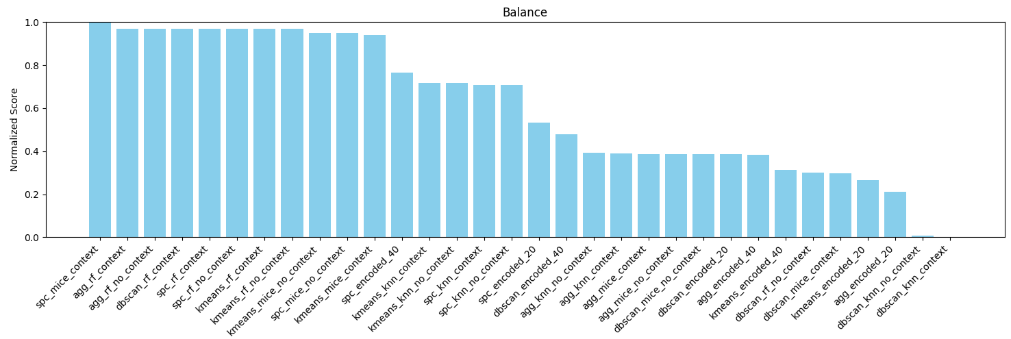
\includegraphics[width=\textwidth,height=0.45\textheight,keepaspectratio]{image1_a.png}
  \caption[Normalised Balance scores across all 32 pipelines]{Normalised Balance scores across all 32 clustering pipelines. Higher bars indicate more even cluster-size distribution; DBSCAN and encoded baselines cluster near the bottom.}
  \label{fig:normalized_balance_scores_acro}
\end{figure}

\subsubsection{Silhouette Score}

Silhouette (Figure~\ref{fig:normalized_silhouette_scores_a}) discriminates strongly among pipelines and plays a major role in ranking separation. Spectral and K-Means with imputation --- especially no-context variants --- dominate the upper range, indicating compact, well-separated clusters. Encoded baselines and DBSCAN pipelines frequently produce near-zero or negative silhouette values, signalling overlapping or poorly defined clusters; silhouette therefore strongly reinforces the dominance of imputed pipelines in the composite ranking.

\begin{figure}[!htb]
  \centering
  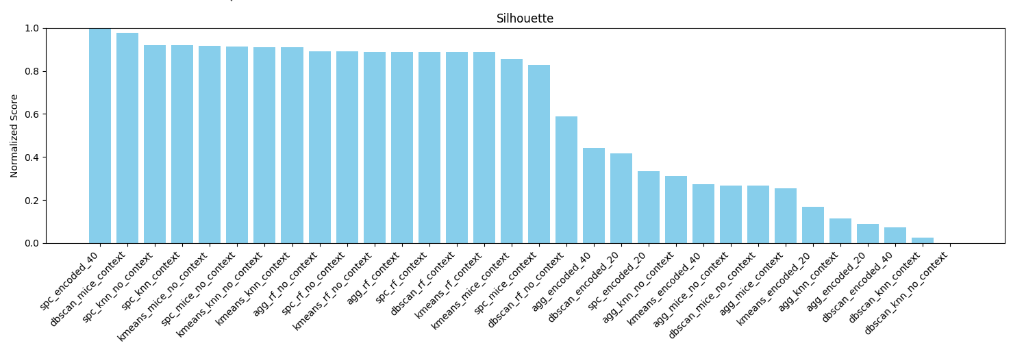
\includegraphics[width=\textwidth,height=0.45\textheight,keepaspectratio]{image1_b.png}
  \caption[Normalised Silhouette scores across all 32 pipelines]{Normalised Silhouette scores across all 32 clustering pipelines. Higher values indicate more cohesive and better-separated clusters; Spectral and K-Means with imputation dominate the upper range, while encoded baselines and DBSCAN cluster near zero or below.}
  \label{fig:normalized_silhouette_scores_a}
\end{figure}

\subsubsection{Calinski--Harabasz Index}

Calinski--Harabasz (Figure~\ref{fig:normalized_calinski_harabasz_i}) sharply distinguishes high-quality global cluster structure from weak or degenerate solutions. Imputed K-Means, Spectral, and Agglomerative pipelines achieve values several orders of magnitude higher than encoded and DBSCAN-based cases; the metric particularly favours centroid-based and hierarchical methods on well-imputed feature spaces. Extremely low Calinski--Harabasz values among DBSCAN and encoded cases contribute heavily to their low composite scores, making this a major driver of top--bottom separation.

\begin{figure}[!htb]
  \centering
  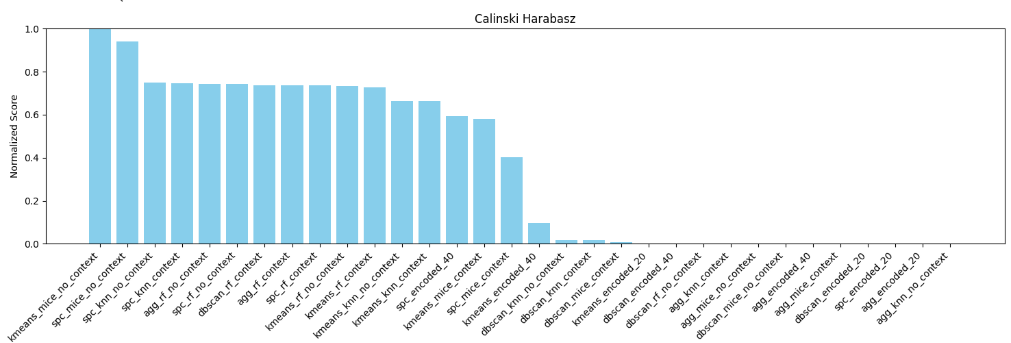
\includegraphics[width=\textwidth,height=0.45\textheight,keepaspectratio]{image1_c.png}
  \caption[Normalised Calinski--Harabasz index across all 32 pipelines]{Normalised Calinski--Harabasz index across all 32 clustering pipelines (variance-ratio criterion; higher is better). Imputed K-Means, Spectral, and Agglomerative cases sit several orders of magnitude above DBSCAN and encoded baselines.}
  \label{fig:normalized_calinski_harabasz_i}
\end{figure}

\subsubsection{Dunn Index}

The Dunn index (Figure~\ref{fig:normalized_dunn_index_across_a}) is highly skewed: only a small subset of cases achieves meaningful values. Agglomerative and Spectral pipelines with MissForest imputation stand out, producing exceptionally high Dunn scores that indicate strong minimum inter-cluster separation relative to cluster diameter; most other pipelines --- including K-Means and all encoded baselines --- yield values near zero. Because Dunn is sensitive to minimum-distance relationships, it rewards structurally clean cluster solutions and disproportionately boosts the top-ranked imputed cases.

\begin{figure}[!htb]
  \centering
  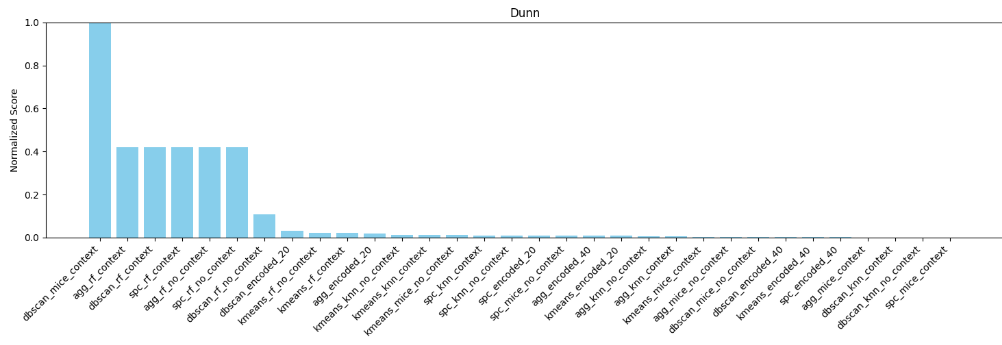
\includegraphics[width=\textwidth,height=0.45\textheight,keepaspectratio]{image1_d.png}
  \caption[Normalised Dunn index across all 32 pipelines]{Normalised Dunn index across all 32 clustering pipelines (ratio of minimum inter-cluster distance to maximum intra-cluster diameter; higher is better). Only a few imputed Agglomerative and Spectral pipelines stand out clearly above the near-zero floor.}
  \label{fig:normalized_dunn_index_across_a}
\end{figure}

\subsubsection{Davies--Bouldin Index}

Davies--Bouldin (Figure~\ref{fig:normalized_davies_bouldin_inde}; inverted for comparability) shows patterns broadly consistent with silhouette and Dunn. Imputed Spectral and K-Means pipelines achieve favourable scores, indicating low average cluster similarity, while encoded and DBSCAN-based pipelines perform poorly. The index does not fully reorder the rankings on its own but reinforces penalties for noisy or overlapping cluster structures and contributes to the demotion of DBSCAN and baseline cases.

\begin{figure}[!htb]
  \centering
  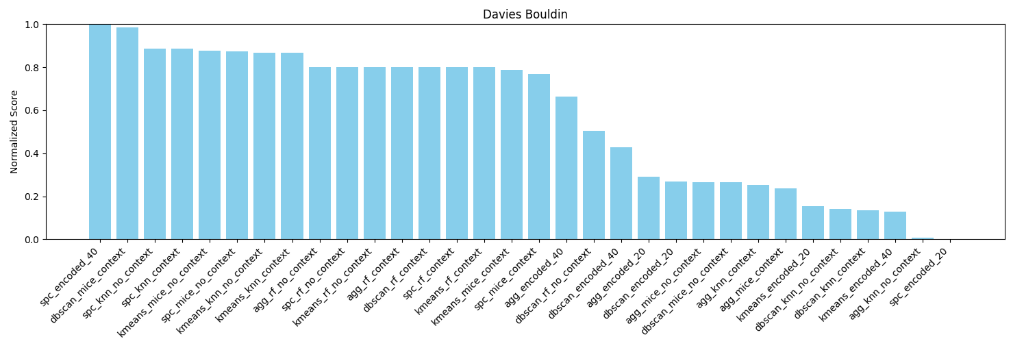
\includegraphics[width=\textwidth,height=0.45\textheight,keepaspectratio]{image1_e.png}
  \caption[Normalised Davies--Bouldin index across all 32 pipelines]{Normalised Davies--Bouldin index across all 32 clustering pipelines (inverted so that higher bars indicate better separation between clusters). Patterns broadly mirror the silhouette and Dunn distributions.}
  \label{fig:normalized_davies_bouldin_inde}
\end{figure}

\subsubsection{Xie--Beni Index}

Xie--Beni (Figure~\ref{fig:normalized_xie_beni_index_acro}) strongly favours imputed pipelines, particularly those using MissForest and MICE, across both context settings. High-performing cases show low intra-cluster variance relative to inter-cluster separation, while encoded and DBSCAN configurations score near zero after normalisation. The metric is especially effective at identifying degenerate clustering outcomes such as tiny or highly scattered clusters and closely tracks the final composite ranking.

\begin{figure}[!htb]
  \centering
  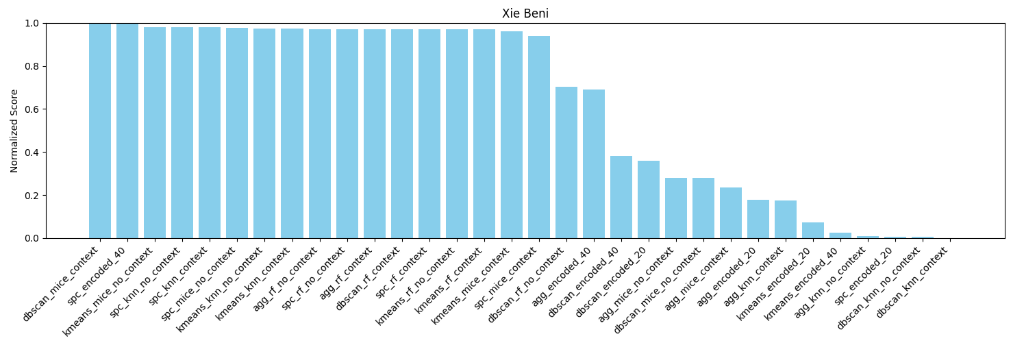
\includegraphics[width=\textwidth,height=0.45\textheight,keepaspectratio]{image1_f.png}
  \caption[Normalised Xie--Beni index across all 32 pipelines]{Normalised Xie--Beni index across all 32 clustering pipelines (inverted; higher is better). The distribution closely tracks the final composite ranking, with imputed MissForest and MICE pipelines at the top.}
  \label{fig:normalized_xie_beni_index_acro}
\end{figure}

\subsection{Group Average Comparisons}

To complement the case-level analysis, group-level averages were computed by aggregating metrics across predefined groups, exposing systematic effects of imputation strategy, predictor context, and clustering algorithm.

\subsubsection{Comparison of Imputation Strategies}

MissForest substantially outperforms all other strategies (Figure~\ref{fig:average_metric_comparison_acro}), achieving the highest average balance (0.64), silhouette (0.70), Calinski--Harabasz (8481), Dunn (0.66), Xie--Beni (0.93), and composite score (23.27). MICE shows moderate gains over non-imputed baselines, particularly in balance and Dunn, but is clearly inferior to MissForest. KNN performs inconsistently, with low Dunn (0.02) and weaker silhouette values, reflecting sensitivity to local noise. Non-imputed datasets rank worst across all metrics, confirming that imputation is essential for stable clustering in this setting.

\begin{figure}[!htb]
  \centering
  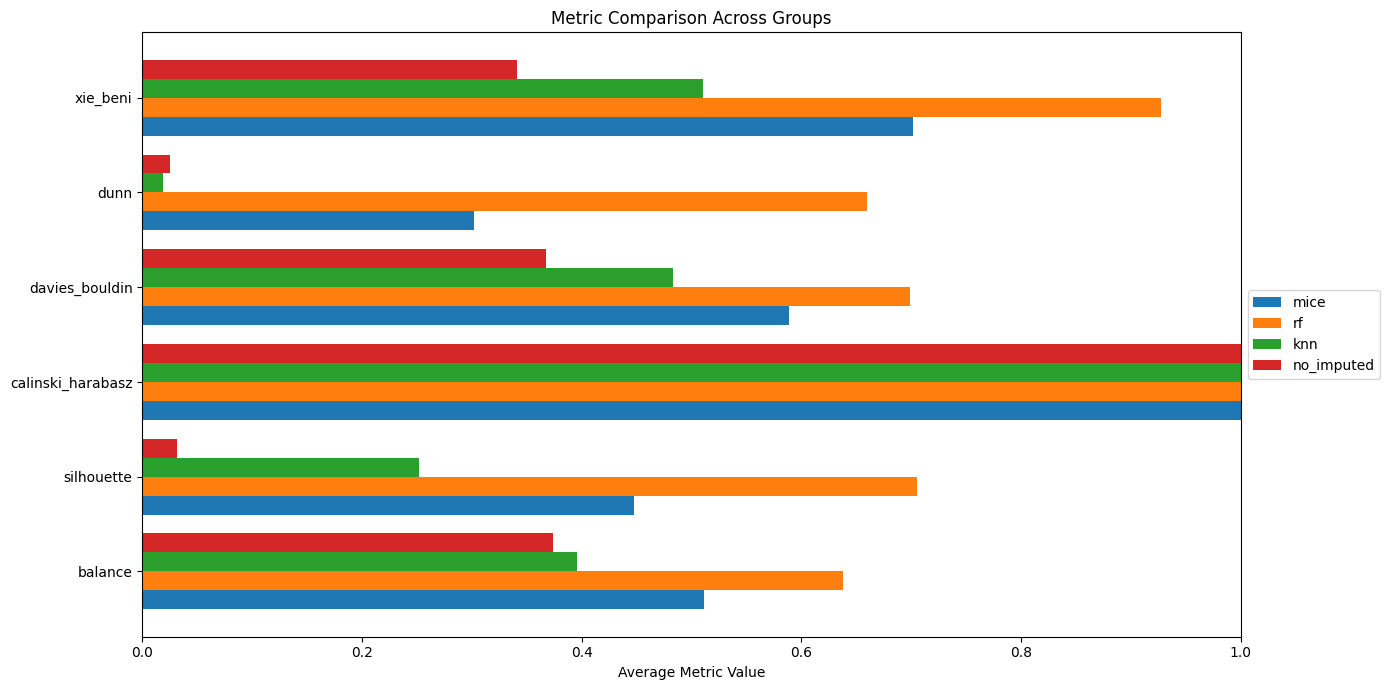
\includegraphics[width=\textwidth,height=0.6\textheight,keepaspectratio]{image12.png}
  \caption[Average metric comparison across imputation strategies]{Average metric comparison across the four imputation strategies (MissForest, MICE, KNN, and non-imputed baseline). Each grouped bar reports the mean of one normalised metric across all pipelines using that strategy; MissForest leads on every metric and on the composite score.}
  \label{fig:average_metric_comparison_acro}
\end{figure}

\subsubsection{Context-Aware vs.\ No-Context Imputation}

Context-aware imputation (Figure~\ref{fig:average_metric_comparison_betw}) yields higher averages for silhouette (0.51 vs.\ 0.43), Dunn (0.45 vs.\ 0.20), and Xie--Beni (0.76 vs.\ 0.67), suggesting improved cluster separation and compactness when irrelevant predictors are excluded. No-context imputation achieves a slightly higher Calinski--Harabasz score (6137 vs.\ 5869), indicating that additional features may inflate variance-based separation even if they introduce noise; balance scores are comparable across both groups. Overall, context-aware imputation attains a marginally higher average composite score (18.55 vs.\ 18.18) --- a small but consistent advantage.

\begin{figure}[!htb]
  \centering
  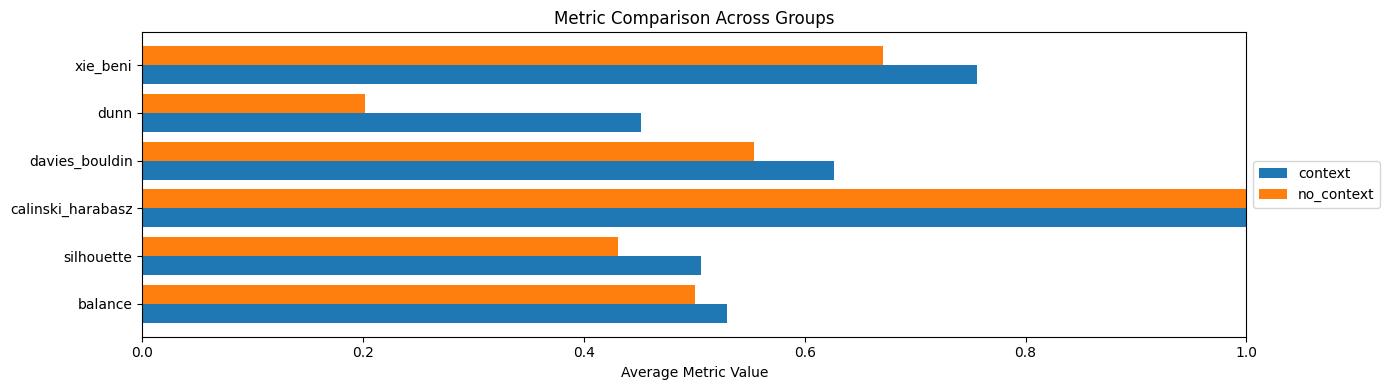
\includegraphics[width=\textwidth,height=0.45\textheight,keepaspectratio]{image19.png}
  \caption[Average metric comparison: context-aware vs.\ no-context imputation]{Average metric comparison between context-aware and no-context imputation strategies. Each grouped bar reports the mean of one normalised metric over all pipelines in the corresponding strategy group; context-aware imputation leads on silhouette, Dunn, and Xie--Beni.}
  \label{fig:average_metric_comparison_betw}
\end{figure}

\subsubsection{Comparison of Clustering Algorithms}

Spectral achieves the highest average performance across most metrics (Figure~\ref{fig:average_metric_comparison_algo}), including silhouette (0.68), Calinski--Harabasz (8084), balance (0.60), and Xie--Beni (0.85), leading to the highest average composite score (22.18). K-Means is competitive, particularly in balance (0.55) and Calinski--Harabasz (7346), but suffers from extremely low Dunn values (0.03), indicating weak minimum inter-cluster separation. Agglomerative shows moderate balance and Dunn performance but lower silhouette overall, and DBSCAN exhibits the weakest average performance --- low balance and silhouette despite a relatively higher Dunn index, reflecting its sensitivity to parameter settings and difficulty with varying densities.

\begin{figure}[!htb]
  \centering
  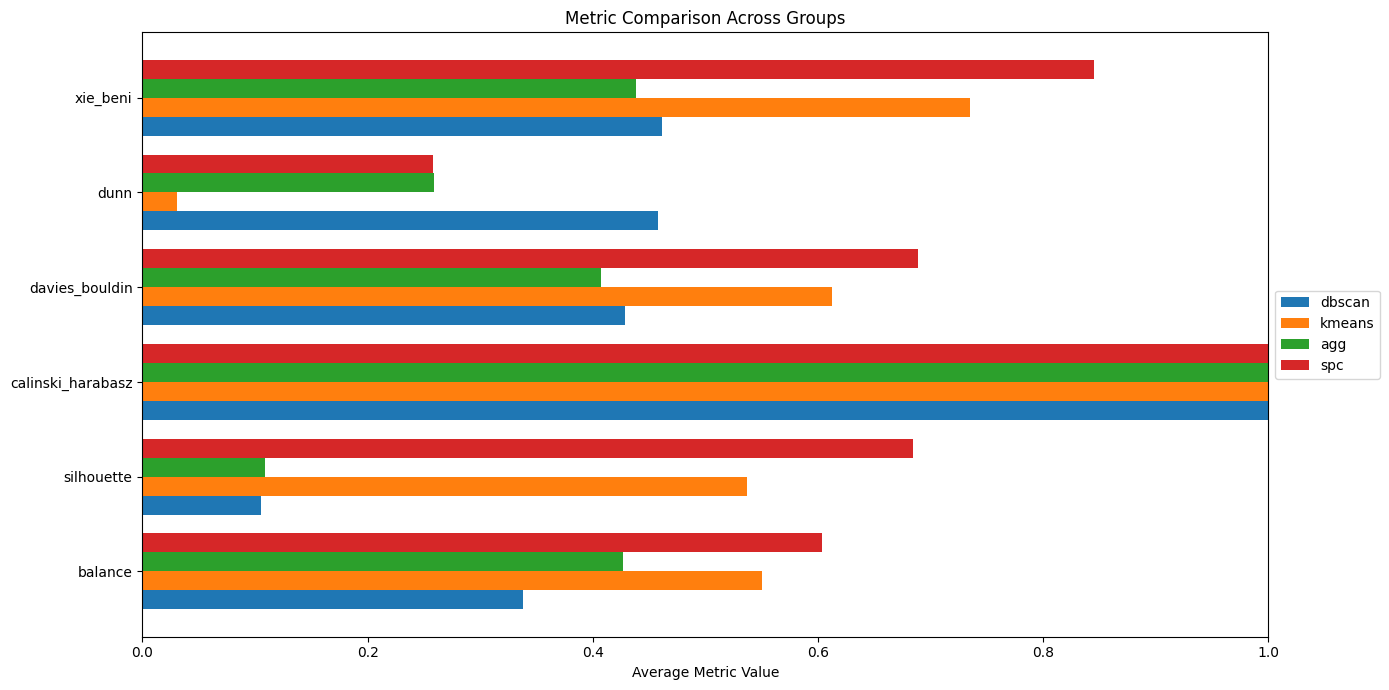
\includegraphics[width=\textwidth,height=0.6\textheight,keepaspectratio]{image10.png}
  \caption[Average metric comparison across clustering algorithms]{Average metric comparison across the four clustering algorithms (K-Means, Agglomerative, DBSCAN, Spectral). Each grouped bar reports the mean of one normalised metric over all pipelines using that algorithm; Spectral leads on most metrics and on the overall composite score.}
  \label{fig:average_metric_comparison_algo}
\end{figure}

\section{Key Takeaways}

The comparative evaluation across imputation strategies, context settings, clustering algorithms, and metrics yields four headline observations.

\begin{itemize}
  \item \textbf{Imputation matters.} Imputed pipelines substantially outperform non-imputed baselines (avg.\ 10.90). MissForest is strongest (avg.\ 23.27), followed by MICE (16.91) and KNN (14.92), confirming tree-based imputation as more stable on this data type.
  \item \textbf{Context-awareness adds little.} Context-aware pipelines slightly edge no-context (18.55 vs.\ 18.18); several top pipelines are non-context-aware, indicating that with strong imputation the full feature set remains advantageous.
  \item \textbf{Algorithm averages.} Spectral (22.18) and K-Means (18.80) outperform Agglomerative (13.28) and DBSCAN (11.74) on average. Agglomerative produces the single best pipeline but is more preprocessing-sensitive; DBSCAN is weakest, consistent with its instability under imbalance and noise.
  \item \textbf{Balance and Silhouette dominate the ranking.} They effectively penalise imbalanced or poorly separated clusters, which is why pipelines with strong individual Dunn or Davies--Bouldin scores can still rank poorly overall.
\end{itemize}

\textbf{A note on score margins.} The top four pipelines (\texttt{agg\_rf\_no\_context} $=$ 27.30, \texttt{kmeans\_mice\_no\_context} $=$ 26.60, \texttt{agg\_rf\_context} $=$ 26.35, \texttt{spc\_rf\_no\_context} $=$ 25.60) span a composite range of roughly 1.7 points on a 1--32 scale. With $n \approx 1{,}600$ records and a single hold-out run per pipeline, we did not compute bootstrap confidence intervals or permutation tests on the composite differences, and we therefore do not claim that these top-ranked pipelines are statistically distinguishable from one another. The ranking should be read as a robust separation between clearly strong and clearly degenerate pipelines --- the top quartile is well separated from the bottom quartile, which contains DBSCAN-noise solutions scoring 4--12 --- rather than as a strict ordering within the top group. The detailed profile in \S4.6 uses \texttt{agg\_rf\_no\_context} as a representative best pipeline for that reason: it sits at the top of a near-tied cluster of strong solutions, not as a uniquely optimal choice. Resampling-based uncertainty quantification on the composite score is recommended for any subsequent replication (see \S6.5).

Table~\ref{tbl:best_pipeline_per_group} summarises the best pipeline per comparison group.

\begin{table}[H]
\centering
\caption[Best pipeline per comparison group]{Best-performing pipeline for each comparison group.}
\label{tbl:best_pipeline_per_group}
\renewcommand{\arraystretch}{1.0}
\small
\begin{tabularx}{\textwidth}{|>{\hsize=0.869\hsize\linewidth=\hsize\raggedright\arraybackslash}X|>{\hsize=0.979\hsize\linewidth=\hsize\raggedright\arraybackslash}X|>{\hsize=1.243\hsize\linewidth=\hsize\raggedright\arraybackslash}X|>{\hsize=0.909\hsize\linewidth=\hsize\raggedright\arraybackslash}X|}
\hline
\textbf{Group Type} & \textbf{Group Name} & \textbf{Best Pipeline} & \textbf{Composite Score} \\ \hline
Algorithm & Agglomerative & agg\_\hspace{0pt}rf\_\hspace{0pt}no\_\hspace{0pt}context & 27.30 \\ \hline
Algorithm & K-Means & kmeans\_\hspace{0pt}mice\_\hspace{0pt}no\_\hspace{0pt}context & 26.60 \\ \hline
Algorithm & DBSCAN & dbscan\_\hspace{0pt}rf\_\hspace{0pt}context & 25.15 \\ \hline
Algorithm & Spectral & spc\_\hspace{0pt}rf\_\hspace{0pt}no\_\hspace{0pt}context & 25.60 \\ \hline
Imputation & MissForest (RF) & agg\_\hspace{0pt}rf\_\hspace{0pt}no\_\hspace{0pt}context & 27.30 \\ \hline
Imputation & MICE & kmeans\_\hspace{0pt}mice\_\hspace{0pt}no\_\hspace{0pt}context & 26.60 \\ \hline
Imputation & KNN & spc\_\hspace{0pt}knn\_\hspace{0pt}no\_\hspace{0pt}context & 24.10 \\ \hline
Imputation & No Imputation & spc\_\hspace{0pt}encoded\_\hspace{0pt}40 & 22.80 \\ \hline
Context & Context-aware & agg\_\hspace{0pt}rf\_\hspace{0pt}context & 26.35 \\ \hline
Context & No-context & agg\_\hspace{0pt}rf\_\hspace{0pt}no\_\hspace{0pt}context & 27.30 \\ \hline
\end{tabularx}
\end{table}

\section{Detailed Profiling of the Top-Ranked Cluster}

The best-performing pipeline, \texttt{agg\_rf\_no\_context} (Agglomerative Clustering with MissForest no-context imputation), was selected for deeper inspection. It produced two clusters --- Cluster~0 with 759 records and Cluster~1 with 858 records --- with no overlap and no noise points, partitioning all 1{,}617 records (Figures~\ref{fig:grid_of_pca_reduced_scatter_pl} and~\ref{fig:horizontal_bar_graph_showing_t}). The composite score of 27.30, supported by a balance of 0.685 and silhouette of 0.756, indicates both strong separation and well-balanced cluster sizes. Label-encoded categorical features were decoded using the JSON mappings saved during preprocessing, restoring original semantic values for the cluster-level comparisons that follow.

\subsection{Numerical Feature Profiling}

Table~\ref{tbl:present_summary_statistics_mea} reports summary statistics (mean, median) for all numerical features across the two clusters. Figures~\ref{fig:comparing_age_for_two_clusters} and~\ref{fig:comparing_feels_like_for_two_c} present distribution plots for selected variables with the strongest separation and domain relevance.

\begin{table}[H]
\centering
\caption[Summary statistics for numerical features by cluster]{Summary statistics (mean, median) for all numerical features across the two clusters. Temperature columns appear in Kelvin for Cluster~0 and Celsius for Cluster~1; see the surrounding discussion for the source-cohort caveat.}
\label{tbl:present_summary_statistics_mea}
\renewcommand{\arraystretch}{1.0}
\small
\begin{tabularx}{\textwidth}{|>{\hsize=1.189\hsize\linewidth=\hsize\raggedright\arraybackslash}X|>{\hsize=0.906\hsize\linewidth=\hsize\raggedright\arraybackslash}X|>{\hsize=0.905\hsize\linewidth=\hsize\raggedright\arraybackslash}X|}
\hline
\textbf{Feature} & \textbf{Cluster 0 (n=759)} & \textbf{Cluster 1 (n=858)} \\ \hline
Age (mean / median) & 28.00 / 24.00 & 25.80 / 23.00 \\ \hline
Feels like (mean / median) & 299.89 / 300.65 & 290.46 / 290.44 \\ \hline
Temp min (mean / median) & 298.95 / 299.51 & 23.78 / 25.61 \\ \hline
Temp max (mean / median) & 298.95 / 299.51 & 31.80 / 32.54 \\ \hline
Air pressure (mean / median) & 1004.77 / 1004.00 & 1007.01 / 1005.90 \\ \hline
Humidity (mean / median) & 85.19 / 87.00 & 71.71 / 70.11 \\ \hline
Wind speed (mean / median) & 3.52 / 3.00 & 7.27 / 7.20 \\ \hline
Wind direction (mean / median) & 149.05 / 145.00 & 193.32 / 194.53 \\ \hline
Cloud cover (mean / median) & 64.05 / 75.00 & 60.68 / 67.70 \\ \hline
Latitude (mean / median) & 23.89 / 23.92 & 23.67 / 23.76 \\ \hline
Longitude (mean / median) & 90.11 / 90.01 & 90.26 / 90.36 \\ \hline
Day (mean / median) & 16.78 / 16.00 & 14.72 / 15.00 \\ \hline
Month (mean / median) & 7.22 / 7.00 & 5.69 / 6.00 \\ \hline
Year (mean / median) & 2020 / 2020 & 2021.96 / 2022 \\ \hline
Week (mean / median) & 30.12 / 30.00 & 22.76 / 23.00 \\ \hline
\end{tabularx}
\end{table}

Age distributions show a modest demographic contrast between the two clusters, with one consistently exhibiting slightly higher average values (Figure~\ref{fig:comparing_age_for_two_clusters}). The temperature-related variable \texttt{feels\_like} shows the largest apparent separation (Figure~\ref{fig:comparing_feels_like_for_two_c}); however, the magnitude of this contrast is largely an artefact of unit inconsistency between the two source cohorts (Kelvin for the Cluster~0 records, which come from the 2020 Kaggle subset, and Celsius for the Cluster~1 records, which come from the manually collected 2017--2025 cases) and should not be read as a substantive environmental finding. The identical \texttt{temp\_min} and \texttt{temp\_max} values in Cluster~0 are a source-data artefact of the Kaggle subset rather than a computation error. Secondary environmental features (air humidity, wind speed) show consistent but less pronounced separation, again co-varying with the cohort split and subject to the source-confound caveat developed in \S\ref{sec:source_cohort_caveat}. With those caveats in place, the patterns are best read as cohort-aligned feature contrasts that warrant further investigation against more homogeneously sourced data.

\begin{figure}[!htb]
  \centering
  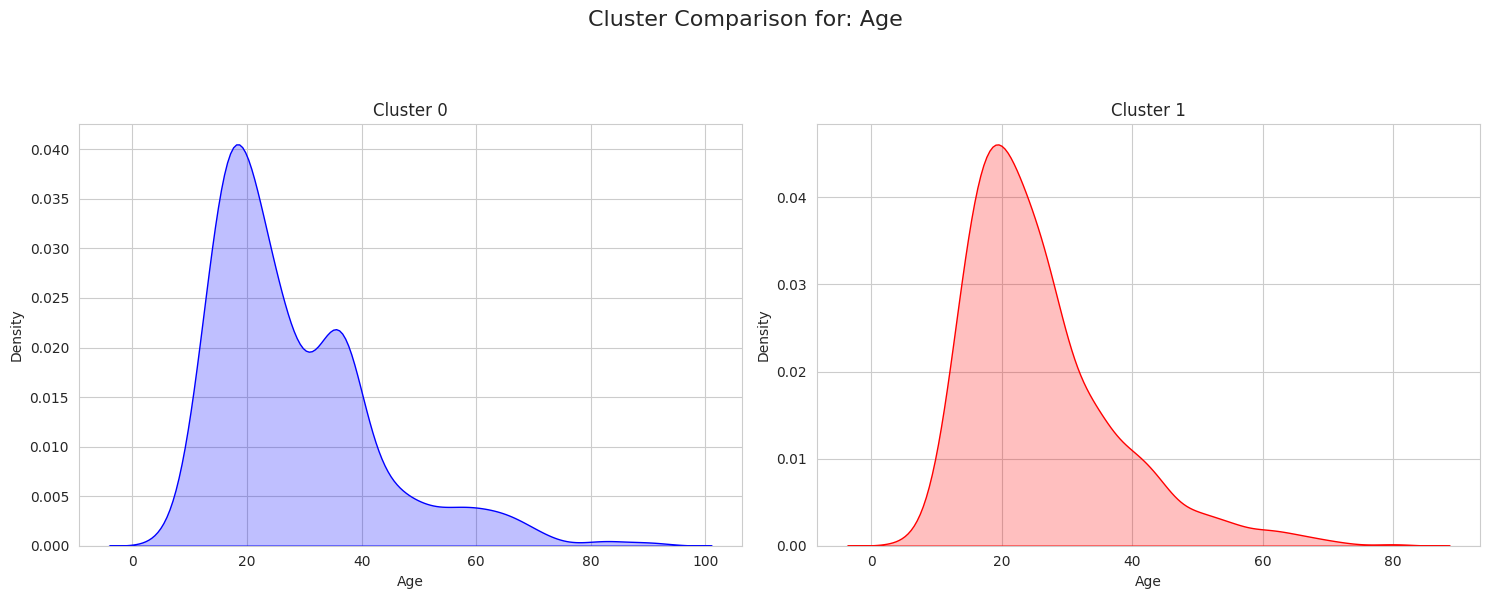
\includegraphics[width=\textwidth,height=0.6\textheight,keepaspectratio]{image11.png}
  \caption[Comparing age for two clusters]{Comparing age for two clusters}
  \label{fig:comparing_age_for_two_clusters}
\end{figure}

\begin{figure}[!htb]
  \centering
  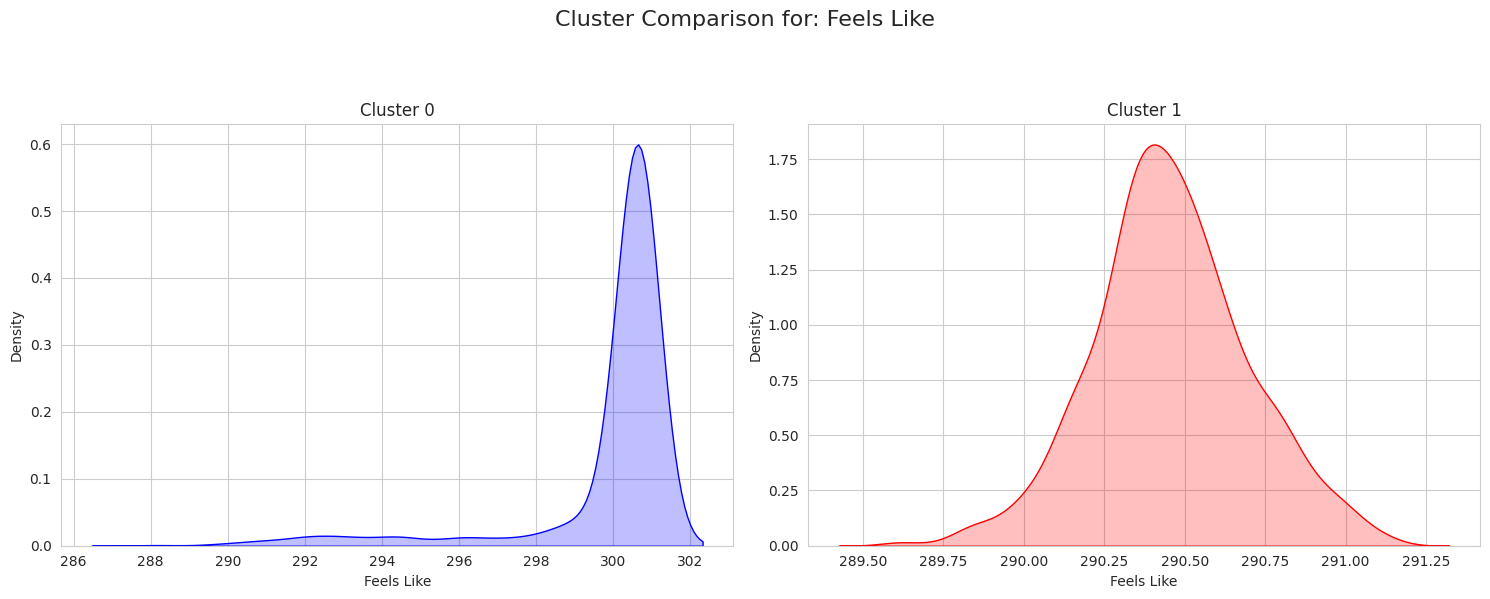
\includegraphics[width=\textwidth,height=0.6\textheight,keepaspectratio]{image17.png}
  \caption[Comparing feels\_like for two clusters]{Comparing feels\_like for two clusters}
  \label{fig:comparing_feels_like_for_two_c}
\end{figure}

Complete numerical feature comparisons for all variables appear in Figure~\ref{fig:appendix_numerical_all}.

\subsection{Categorical Feature Profiling}

Categorical feature distributions were analysed to uncover social and contextual differences between clusters. Table~\ref{tbl:categorical_modes_two_clusters} reports the most frequent categories, while Figures~\ref{fig:comparing_reason_for_two_clust} and~\ref{fig:comparing_workplace_for_two_cl} focus on the most discriminative variables.

\begin{table}[H]
\centering
\caption[Categorical mode and frequency by cluster]{Most frequent category (mode and percentage) for each categorical feature across the two clusters. The near-deterministic value for Cluster~1's \texttt{weather\_main} (Partly cloudy, 99.9\%) reflects the dominant imputed value for the manually collected 2017--2025 records under MissForest rather than a homogeneous physical weather pattern.}
\label{tbl:categorical_modes_two_clusters}
\renewcommand{\arraystretch}{1.0}
\small
\begin{tabularx}{\textwidth}{|>{\hsize=0.950\hsize\linewidth=\hsize\raggedright\arraybackslash}X|>{\hsize=1.022\hsize\linewidth=\hsize\raggedright\arraybackslash}X|>{\hsize=1.028\hsize\linewidth=\hsize\raggedright\arraybackslash}X|}
\hline
\textbf{Feature} & \textbf{Cluster 0 (Mode, \%)} & \textbf{Cluster 1 (Mode, \%)} \\ \hline
Age group & Teen (48.5\%) & Teen (39.2\%) \\ \hline
Gender & Female (54.8\%) & Male (50.8\%) \\ \hline
Marital status & Married (48.4\%) & Married (47.6\%) \\ \hline
Profession group & Student (37.0\%) & Student (39.7\%) \\ \hline
Workplace & Semi-urban (54.5\%) & Rural (50.0\%) \\ \hline
Religion & Muslim (87.5\%) & Muslim (85.4\%) \\ \hline
Financial condition & Lower (54.3\%) & Lower (57.6\%) \\ \hline
Hometown & Bogura (4.0\%) & Dhaka (9.1\%) \\ \hline
Primary reason & Family issue (23.1\%) & Mental (26.5\%) \\ \hline
Method & Hanging (73.3\%) & Hanging (74.1\%) \\ \hline
Weather (main) & Clouds (38.1\%) & Partly cloudy (99.9\%) \\ \hline
Weather description & Haze (19.6\%) & Haze (64.7\%) \\ \hline
Weekday & Saturday (17.9\%) & Sunday (16.9\%) \\ \hline
Time of day & Night (36.9\%) & Night (35.5\%) \\ \hline
\end{tabularx}
\end{table}

Workplace type varies meaningfully between the two clusters, indicating differences in social and environmental context (Figure~\ref{fig:comparing_workplace_for_two_cl}), and reported reasons for suicide show distinct dominant categories across the partition (Figure~\ref{fig:comparing_reason_for_two_clust}). Further contrasts appear in weather-related features such as \texttt{weather\_main} (e.g., clear, clouds, rain) and \texttt{weather\_description} (e.g., broken clouds, clear sky, haze), indicating additional environmental variation. Full categorical distributions across clusters appear in Figure~\ref{fig:appendix_categorical_all}.

\begin{figure}[!htb]
  \centering
  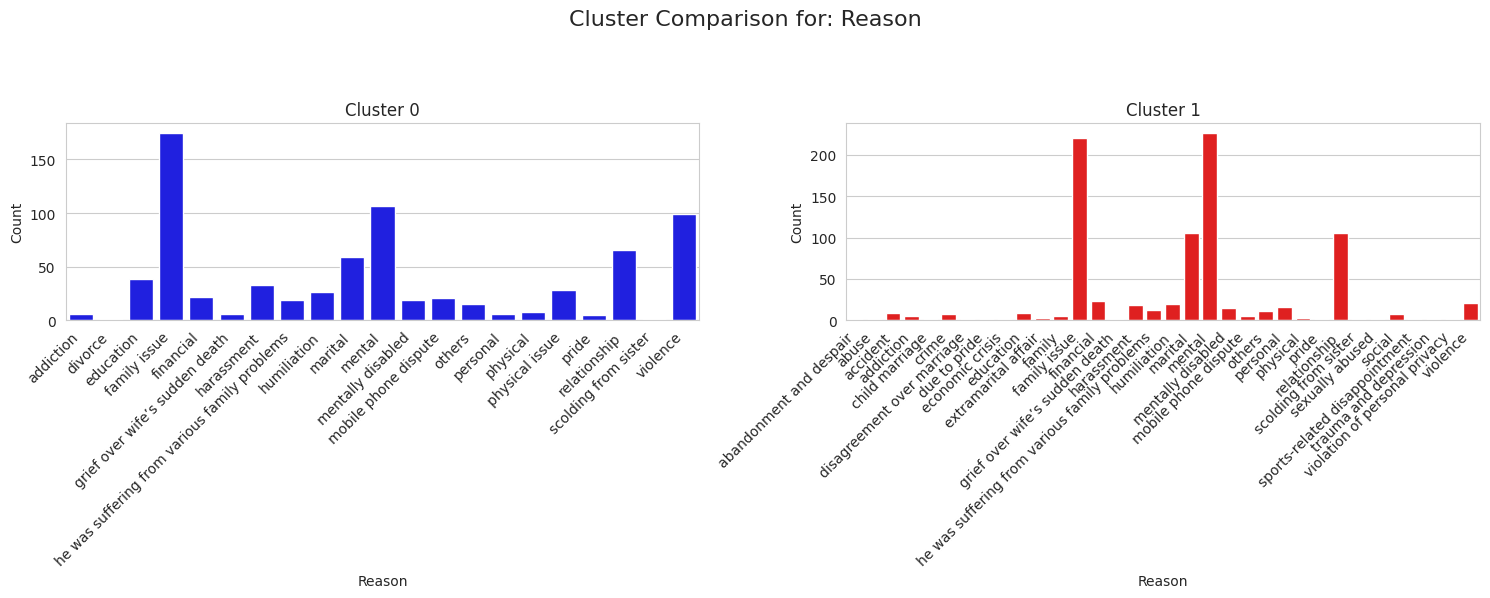
\includegraphics[width=\textwidth,height=0.6\textheight,keepaspectratio]{image15.png}
  \caption[Comparing reason for two clusters]{Comparing reason for two clusters}
  \label{fig:comparing_reason_for_two_clust}
\end{figure}

\begin{figure}[!htb]
  \centering
  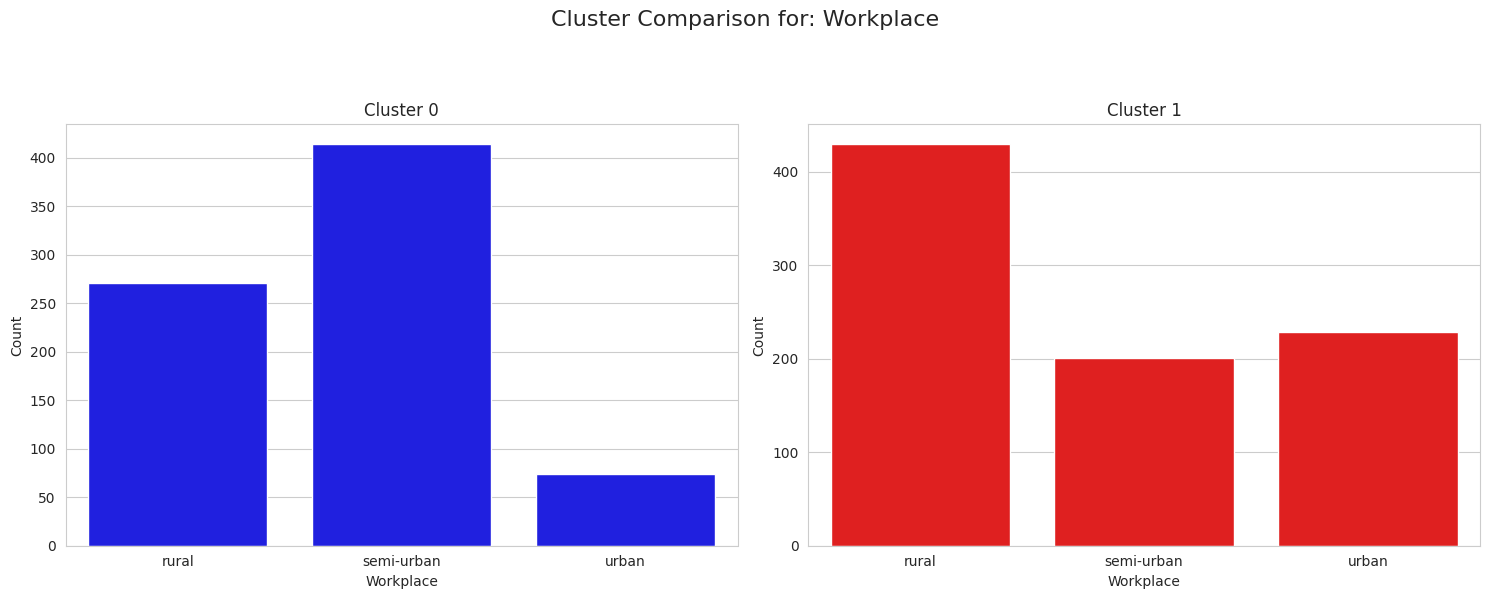
\includegraphics[width=\textwidth,height=0.6\textheight,keepaspectratio]{image24.png}
  \caption[Comparing workplace for two clusters]{Comparing workplace for two clusters}
  \label{fig:comparing_workplace_for_two_cl}
\end{figure}

\subsection{Geographic Profiling}

The geographic distribution of the two clusters is visualised in Figure~\ref{fig:comparing_spatial_density_for} as a latitude--longitude heatmap over Bangladesh, with distinct colours per cluster to emphasise spatial coherence and contrast. The clusters are not spatially arbitrary: Cluster~1 hometowns concentrate at the two largest cities --- Dhaka (9.1\%) and Chattogram (7.7\%) jointly account for nearly one in six cases --- while Cluster~0 hometowns are dispersed more evenly across mid-sized provincial centres (Bogura, Rajshahi, Mymensingh, each $\sim$3--4\%). The two clusters are nonetheless internally heterogeneous on workplace type: the Cluster~1 modal workplace is rural (50.0\%) with a substantial urban tail (26.6\%), while Cluster~0 is dominated by semi-urban workplaces (54.5\%). The pattern is therefore one of \emph{where the cases come from} more than \emph{where they occur}, and reinforces the numerical and categorical findings without flattening the within-cluster variation.

\begin{figure}[!htb]
  \centering
  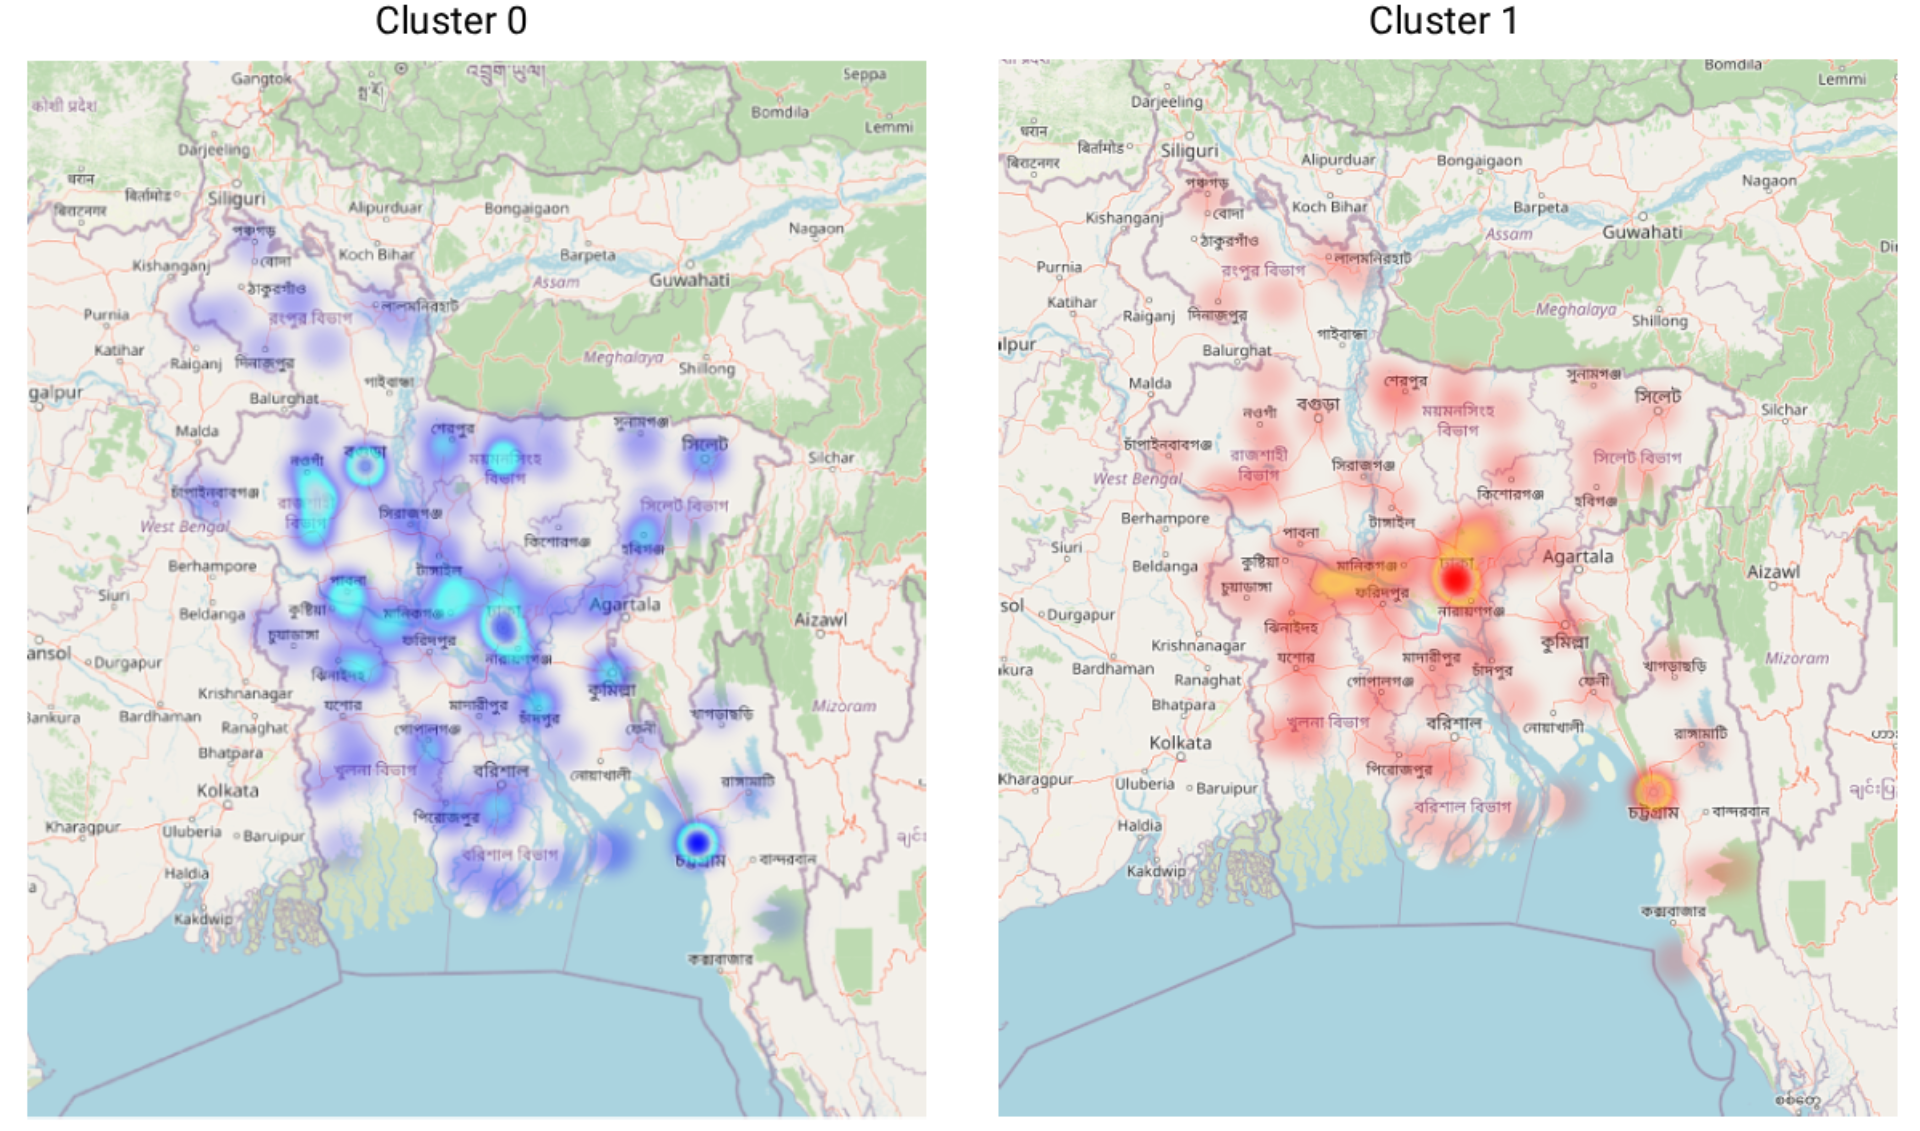
\includegraphics[width=\textwidth,height=0.6\textheight,keepaspectratio]{image18.png}
  \caption[Comparing spatial density for two clusters]{Comparing spatial density for two clusters}
  \label{fig:comparing_spatial_density_for}
\end{figure}

\subsection{Temporal Pattern and Source-Cohort Confound}\label{sec:source_cohort_caveat}

A striking temporal pattern emerged during manual inspection. Cluster~0 contains exclusively records from 2020, whereas Cluster~1 is concentrated in 2017--2019 and 2021--2025 with only a small residue of 2020 cases (Figure~\ref{fig:comparing_years_for_two_cluste}). This separation aligns almost precisely with the dataset construction process: the original Kaggle dataset comprised 760 records all from 2020, and 857 manually collected cases spanning years before and after 2020 were added later with systematically higher missingness across several columns; the partition assigns 759 records to Cluster~0 and 858 to Cluster~1, a single-record cross-over consistent with feature-driven near-perfect cohort separation.

Temporal information was not used as a clustering input --- no year, date, or source field was provided to the algorithm --- so the two-cluster boundary coinciding with the cohort boundary is an emergent property of the feature distributions. As an internal consistency check the result is positive: it shows that the imputation pipeline did not erase cohort-level structure, and that the algorithm is capable of recovering coherent partitions from severely incomplete inputs. As a substantive finding about Bangladeshi suicide patterns, however, it carries a clear caveat: the two cohorts differ systematically in completeness, reporting era, the journalistic and geographic profile of the underlying coverage, and (for temperature-derived variables) raw measurement units. These source-level differences propagate into virtually every downstream feature the clustering operates on. The recovered partition should therefore be characterised as a source-cohort split that co-varies with --- rather than cleanly isolates --- demographic, environmental, and behavioural variation in the underlying population, and any feature-level contrast in this section should be read as exploratory subgroup structure partially confounded with collection source, rather than as the discovery of two intrinsically distinct epidemiological subpopulations. The confound, and the related temperature-unit caveat, are addressed explicitly in \S6.4 (Limitations~\ref{lim:source_cohort} and~\ref{lim:temp_units}).

\begin{figure}[!htb]
  \centering
  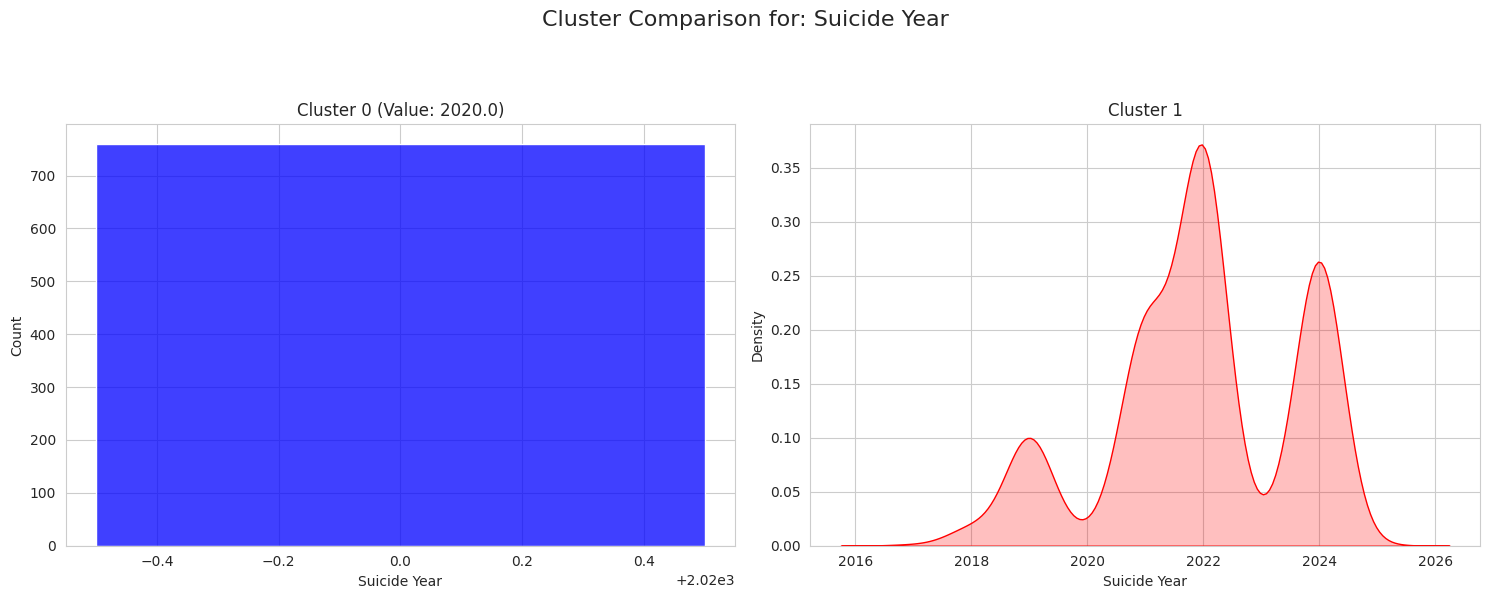
\includegraphics[width=\textwidth,height=0.6\textheight,keepaspectratio]{image20.png}
  \caption[Comparing years for two clusters]{Comparing years for two clusters}
  \label{fig:comparing_years_for_two_cluste}
\end{figure}

\section{Discussion of Findings}\label{sec:discussion_of_findings}

The framework's effectiveness is supported internally by the results. The balance penalty played the role for which it was introduced, consistently demoting noisy or severely imbalanced solutions --- particularly DBSCAN-based pipelines that achieved superficially high geometric scores while assigning the vast majority of points to noise. Without it, the ranking would have been dominated by near-degenerate partitions of little interpretive value. Imputation strategy had a substantial impact: MissForest consistently produced the strongest results on this dataset, both at peak and on average, while non-imputed pipelines performed markedly worse. No-context configurations slightly outperformed context-aware ones on average, consistent with the interpretation that a richer predictor space during imputation provides a modest benefit on this particular feature set; this is a dataset-specific observation rather than a general claim.

The top-ranked pipeline produced clusters whose feature-level differences span demographics, environment, social context, geography, and time. As discussed in detail in \S\ref{sec:source_cohort_caveat}, however, the recovered partition coincides with the dataset's two-cohort construction history, so the temporal separation that emerged without explicit supervision is best read as evidence that the pipeline preserves cohort-level structure under high missingness rather than as evidence that the resulting groups represent distinct intrinsic suicide profiles. Its substantive interpretation is exploratory and partially confounded with collection source. Additional limitations include sensitivity to hyperparameter choices, the substantial computational cost of MissForest, the absence of external ground-truth labels, and the temperature-unit inconsistency between cohorts noted in \S6.4 (Limitation~\ref{lim:temp_units}); these jointly motivate future work on more homogeneously sourced and unit-harmonised data before any cluster-level finding is taken as actionable evidence for prevention practice.

\section{Summary}

The 32-pipeline framework placed \texttt{agg\_rf\_no\_context} (Agglomerative + MissForest no-context) at the top with a composite score of 27.30, followed by MICE and MissForest variants under K-Means and Spectral clustering. Imputation was the dominant performance driver, MissForest the strongest imputer, and DBSCAN the least robust algorithm under the balance-aware composite, while no single metric reordered the ranking on its own: balance and silhouette jointly governed top--bottom separation, with Calinski--Harabasz amplifying it. The detailed profile of the best pipeline yielded a clean two-cluster solution (759 vs.\ 858 records) whose feature-level contrasts span age, environment, workplace, geography, and reporting period, but whose boundary aligns almost exactly with the dataset's two-cohort construction history --- a source-cohort confound that we read as an internal consistency check on the imputation rather than as a substantive epidemiological finding.

% Chapter 5: Standards, Constraints, and Milestones
\chapter{Standards, Constraints, and Milestones}

\section{Sustainability Standards}

Sustainable data-science and public-health research demands that outputs, methods, and data artefacts remain useful, reproducible, and ethically sound beyond the immediate project. The study aligns with the United Nations 2030 Agenda for Sustainable Development \cite{ref24} across three goals relevant to suicide prevention and mental health research.

\textbf{SDG 3 (Good Health and Well-being) --- Target 3.4.} SDG~3.4 calls on member states to reduce premature mortality from non-communicable diseases (NCDs) by one third and to promote mental health and well-being \cite{ref25}, and suicide is tracked explicitly as indicator SDG~3.4.2 (suicide mortality rate, per 100,000 population). Subject to the source-cohort and reported-cases caveats set out in Chapter~4 and \S6.4, the study contributes hypothesis-generating evidence towards this target in Bangladesh by surfacing candidate demographic, geographic, and temporal patterns within the reported-case cohort that warrant follow-up in more homogeneously sourced data --- prerequisites for designing targeted prevention programmes.

\textbf{SDG 5 (Gender Equality) --- Target 5.2.} The cluster-level descriptive statistics in Chapter~4 show that, within the reported-suicide records analysed here, female cases --- particularly young married women and female students associated with family conflict, academic pressure, and relationship-related distress --- form a substantial share of one of the two recovered subgroups. SDG~5 calls for the elimination of all forms of violence against and exploitation of women and girls \cite{ref24}. Subject to the caveats in \S\ref{sec:source_cohort_caveat} and \S6.4 (the cluster split is partly confounded with collection source, and the dataset is drawn from reported cases rather than from a representative population sample), the descriptive evidence here can inform the design of more gender-sensitive mental-health and suicide-prevention research and outreach.

\textbf{SDG 10 (Reduced Inequalities).} The geographic and socioeconomic profiling in this study is consistent with the broader literature on rural--urban inequality in Bangladesh \cite{ref50}, and SDG~10 calls for reducing inequalities within and among countries \cite{ref24}. The cluster-level descriptive identification of rural, low-income, and agriculturally dependent populations within the reported-suicide records provides a starting point --- not a definitive epidemiological estimate --- for directing future research and resource-allocation discussions towards potentially under-served communities.

Beyond SDG alignment, the work was designed for long-term sustainability in three additional ways. Code, preprocessing scripts, and the de-identified dataset will be released publicly under an open-source licence (see \S\ref{sec:data_availability}), enabling other researchers in resource-constrained settings to replicate, extend, or adapt the methodology. The modular 12-notebook architecture means that each component --- data cleaning, imputation, clustering, evaluation --- can be updated independently as new data or improved methods emerge. And the pipeline relies exclusively on free, open-source libraries (scikit-learn, pandas, NumPy, Geopy, Meteostat) and free compute resources (Google Colab), so the framework remains accessible to LMIC researchers without institutional access to commercial software or high-performance computing.

\section{Impacts on Society}

Research on a topic this sensitive carries the potential for significant positive impact and, if handled carelessly, real harm; both dimensions are addressed below.

\textbf{Positive impacts.} The primary intended benefit is the contribution to evidence-based suicide-prevention research in Bangladesh. Machine-learning approaches applied to public-health data are well documented as a means of identifying subgroups that aggregate-level analyses would miss \cite{ref43,ref44,ref53}, and the cluster-level descriptive profiles surfaced here --- contrasting the modal demographic and contextual features of one cohort-aligned cluster against the other --- offer a starting point that stakeholders can use to scope more targeted follow-up research and outreach, subject to the source-confound and data-source biases discussed in \S\ref{sec:source_cohort_caveat} and \S6.4. Table~\ref{tbl:expected_societal_impacts_by_s} summarises potential applications for specific stakeholder groups.

\begin{table}[H]
\centering
\caption[Potential applications by stakeholder group]{Potential applications of cluster-level findings by stakeholder group (presented as hypothesis-generating, subject to source-confound caveats in \S\ref{sec:source_cohort_caveat} and \S6.4).}
\label{tbl:expected_societal_impacts_by_s}
\renewcommand{\arraystretch}{1.0}
\small
\begin{tabularx}{\textwidth}{|>{\hsize=0.611\hsize\linewidth=\hsize\raggedright\arraybackslash}X|>{\hsize=1.389\hsize\linewidth=\hsize\raggedright\arraybackslash}X|}
\hline
\textbf{Stakeholder} & \textbf{Expected Impact} \\ \hline
Ministry of Health and Family Welfare & Evidence-based identification of high-risk demographic groups and geographic districts to prioritise prevention programmes and resource allocation. \\ \hline
NGOs and Mental Health Helplines & Cluster-specific risk profiles enable better targeting of outreach, helpline staffing during high-risk seasons, and community awareness campaigns. \\ \hline
Schools and Universities & Insights into student-specific triggers (academic pressure, exam periods, family conflict) can inform early identification and peer-support programme design. \\ \hline
Rural Development Agencies & Geographic risk profiling highlights high-burden rural districts, supporting targeted livelihood and debt-relief interventions among at-risk populations. \\ \hline
Researchers and Data Scientists & The reproducible 32-pipeline framework and publicly released de-identified dataset provide a methodological foundation for future studies on incomplete social datasets in South Asia. \\ \hline
Media and Journalists & Empirical cluster findings provide a data-driven basis for responsible, non-sensational suicide reporting that highlights structural risk factors rather than individual narratives. \\ \hline
\end{tabularx}
\end{table}

\textbf{Negative impacts and risks.} Algorithmic bias is a well-documented risk in ML applications to public-health data, particularly when training datasets come from non-representative sources \cite{ref45,ref46}. Newspaper-reported cases over-represent urban, female, and more unusual suicide incidents, so any patterns identified through clustering reflect the biases of the source data rather than the true population distribution and should be read as patterns within reported cases, not as prevalence estimates. A second risk is misuse: geographic risk profiling, valuable for resource allocation, could contribute to stigmatising specific districts or demographic groups if communicated irresponsibly. The risk is mitigated by framing all cluster descriptions in terms of structural risk factors (poverty, academic pressure, domestic conflict) rather than intrinsic characteristics of the populations concerned, in line with established ethical guidance on mental-health data communication \cite{ref22}.

\section{Ethical Considerations}

Suicide research is among the most ethically sensitive areas in the social sciences and demands careful attention to privacy, non-maleficence, and the potential for harm to affected communities. The study followed six principles.

\textbf{Privacy and de-identification.} The \texttt{full\_name} column was removed at the earliest preprocessing stage, and the exact address field was standardised to district-level labels only --- a deliberate trade-off that reduces spatial precision while preserving analytical utility. The source URL (\texttt{data\_source} column) was also permanently removed to prevent traceback to individual articles. These measures follow best-practice guidance on psychiatric and behavioural research data \cite{ref22} and constitute de-identification rather than formal $k$-anonymity: the residual combination of district, suicide date, age, and method could, in principle, still re-identify a recent newsworthy case, and the dataset is therefore released under a research-use licence with the explicit caveat that re-users must not attempt re-identification.

\textbf{Sensitive-topic handling.} Method-of-suicide information is retained only in encoded form within the analytical dataset and is never reproduced at the individual case level in any output or visualisation; all cluster profiling is aggregated, consistent with responsible data communication practices for this domain \cite{ref23}.

\textbf{Non-stigmatisation.} Algorithmic pattern-finding can inadvertently reinforce harmful stereotypes about particular groups, so all cluster findings are framed in terms of socioeconomic, environmental, and situational risk factors rather than personal or cultural failings. The language used in cluster labelling and profiling was reviewed to ensure it does not pathologise individuals or communities.

\textbf{Data-source legitimacy.} All newspaper records came from publicly available, freely accessible Bangladeshi news sources; no private medical records, police files, or non-public databases were accessed. The use of publicly available media content for academic suicide research is an established and ethically accepted practice in the field \cite{ref23}.

\textbf{Beneficence.} The overarching ethical justification for the work is its long-term potential to contribute to life-saving prevention. The study aims to produce interpretable subgroup structure that can inform downstream prevention-focused research, not a standalone deployable risk-stratification system, and this orientation shaped methodological choices --- including the decision to prioritise interpretable cluster solutions over those with marginally higher geometric metrics.

\textbf{Algorithmic fairness.} ML models trained on biased data can systematically disadvantage under-represented groups \cite{ref45,ref46}. The balance penalty term introduced here penalises clustering solutions with highly unequal cluster sizes; this is a stability and interpretability safeguard against dominant-cluster artefacts rather than a substantive fairness intervention, and we make no formal fairness-guarantee claim. Imputation and clustering outputs were inspected across demographic subgroups (gender, age group, geographic region) for obvious systematic distortions before finalising cluster profiles.

\section{Challenges Faced}

Implementation involved several technical, methodological, and logistical challenges, summarised in Table~\ref{tbl:key_challenges_encountered_and} with the solutions applied.

\begin{table}[H]
\centering
\caption[Key challenges and solutions]{Key challenges encountered and solutions applied during the research}
\label{tbl:key_challenges_encountered_and}
\renewcommand{\arraystretch}{1.0}
\small
\begin{tabularx}{\textwidth}{|>{\hsize=0.889\hsize\linewidth=\hsize\raggedright\arraybackslash}X|>{\hsize=1.111\hsize\linewidth=\hsize\raggedright\arraybackslash}X|}
\hline
\textbf{Challenge Encountered} & \textbf{Solution Applied} \\ \hline
Extreme missingness ($>$90\%) in several key columns (previous mental health history, family size) & Columns above 70\% missingness permanently excluded; remaining columns treated with three advanced imputation methods under two predictor strategies \\ \hline
Inconsistent Bangla--English spellings and over-granular categorical labels across 13 columns & Iterative manual cleaning and semantic harmonisation; district-level standardisation of hometown reducing cardinality from 594 to 151 unique values \\ \hline
No reliable geocoding service for rural Bangladeshi locations & Geopy with a cached JSON fallback system; lat/long missingness reduced from $\sim$53\% to 6.49\% \\ \hline
Weather API rate limits and missing records for remote locations & Hourly-to-daily fallback strategy with extensive local caching; partial reduction in weather-variable missingness \\ \hline
High computational cost of MissForest imputation (100 trees $\times$ 29 label-encoded features $\times$ 1{,}617 rows, repeated per variant) & Cached intermediate outputs and modular notebook structure enabling incremental execution on the free Colab tier without losing progress \\ \hline
Standard clustering validity metrics favoured geometrically tight but practically useless solutions (e.g.\ DBSCAN with 99\% noise) & Study-specific balance penalty term weighted at 35\% in the composite score, demoting imbalanced and noise-heavy solutions \\ \hline
Choosing encoding for 13 heterogeneous categorical variables with widely different cardinalities & Four encoding strategies applied by feature type: ordinal for ordered features, one-hot for low-cardinality nominals, frequency for high-cardinality nominals, and label encoding for MissForest \\ \hline
\end{tabularx}
\end{table}

The most consequential of these was the evaluation problem: certain DBSCAN configurations produced silhouette scores above 0.87 while clustering only 6 records out of 1{,}617 --- technically high yet practically worthless. The observation, made during early manual inspection of the 32 pipeline outputs, directly motivated the balance metric and was the defining methodological insight that shaped the evaluation framework, illustrating the broader risk of relying on a single metric for unsupervised evaluation in applied social-science contexts.

\section{Constraints}

Alongside the technical challenges, the research operated under structural constraints summarised in Table~\ref{tbl:structural_constraints_affecti}.

\begin{table}[H]
\centering
\caption[Structural constraints affecting scope and generalisability]{Structural constraints affecting the scope and generalisability of the research}
\label{tbl:structural_constraints_affecti}
\renewcommand{\arraystretch}{1.0}
\small
\begin{tabularx}{\textwidth}{|>{\hsize=0.447\hsize\linewidth=\hsize\raggedright\arraybackslash}X|>{\hsize=1.553\hsize\linewidth=\hsize\raggedright\arraybackslash}X|}
\hline
\textbf{Constraint Type} & \textbf{Description} \\ \hline
Data & Limited to newspaper-reported completed suicides only. Suicide attempts, unreported cases, and clinical or police records are not captured, introducing systematic under-coverage bias. \\ \hline
Geographical & Rural areas are under-represented because local and vernacular newspapers are harder to access digitally, and remote incidents receive less media coverage. \\ \hline
Temporal & Data spans 2017--2025; long-term secular trends and pre-2017 patterns cannot be analysed, and the dataset is not updated in real time. \\ \hline
Methodological & Limited to unsupervised exploratory subgroup analysis; no supervised prediction model is developed, and no external ground-truth labels are available to validate cluster assignments. \\ \hline
Hardware and Budget & Pipeline executed on free, student-tier resources (Google Colab, GitHub); MissForest was the dominant runtime cost in the imputation stage and bounded the number of hyperparameter combinations that could be explored. \\ \hline
Language & Bangla free-text columns (e.g.\ \texttt{profession\_description}, \texttt{reason\_description}) could not be processed with standard NLP tools and were excluded. \\ \hline
\end{tabularx}
\end{table}

The data constraint is the most consequential: because the dataset is drawn exclusively from newspaper-reported completed suicides, the findings cannot be generalised to suicide attempts, unreported deaths, or cases that received no media coverage. This structural bias is inherent to newspaper-based suicide research in LMICs \cite{ref23} and is the primary caveat any policymaker or practitioner using these findings should bear in mind.

\section{Project Timeline and Milestones}

The research was conducted over 25 weeks. Figure~\ref{fig:gantt_timeline} presents the project timeline as a Gantt chart organised by week across the nine major task groups; all milestones were met within the planned duration. The most time-intensive phases were the manual data collection (weeks 4--7) --- which required careful per-case verification against multiple source articles --- and the imputation implementation (weeks 15--18), which required not only three distinct imputation algorithms under two predictor strategies but also custom post-imputation processing (one-hot group correction, ordinal rounding) to keep all six imputed datasets analytically coherent. The clustering experiments (weeks 19--21) were the most computationally demanding phase, with grid search and fine-tuning across up to 20 parameter combinations per algorithm per dataset; the final evaluation and profiling phase (weeks 22--23) was the most analytically intensive, covering the composite scoring framework, group-level comparisons, and full decoding and interpretation of the best-performing cluster solution.

\begin{figure}[H]
  \centering
  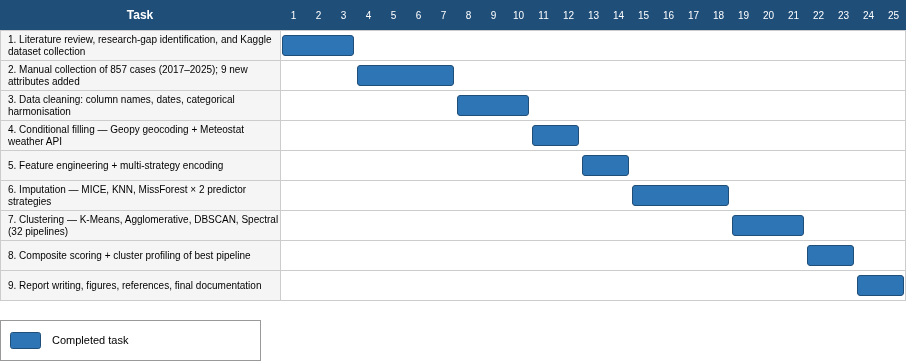
\includegraphics[width=\textwidth,height=0.55\textheight,keepaspectratio]{gantt_timeline.png}
  \caption[Project timeline across 25 weeks and nine task groups]{Project timeline Gantt chart spanning 25 weeks across nine task groups (literature review and base data collection, manual case expansion, data cleaning, conditional API filling, feature engineering and encoding, six-variant imputation, four-algorithm clustering, composite scoring and cluster profiling, and report writing). All tasks completed within the planned schedule.}
  \label{fig:gantt_timeline}
\end{figure}

\section{Data and Code Availability}\label{sec:data_availability}

Following the open and replicable orientation declared above, all artefacts required to reproduce the study are released publicly. The expanded dataset (1{,}617 records, 2017--2025, including the nine added socio-economic and clinical attributes), the twelve Colab notebooks that constitute the pipeline (\texttt{0\_preprocessing} through \texttt{11\_comparing\_clustering}), the per-stage intermediate datasets (\texttt{0\_original.xlsx} through \texttt{11\_forest\_no\_context.xlsx}, plus per-algorithm clustering outputs in \texttt{datasets/\{agg, kmeans, dbscan, spc\}/}), and the cached geocoding and weather responses are distributed together, so any stage can be re-run independently of the original API services. The repository is available at \url{https://github.com/akashmony01/imputation-clustering-comparison}. The source code is released under the MIT License and the dataset under the Creative Commons Attribution 4.0 International (CC-BY 4.0) licence, with the ethical safeguards described in the Ethical Considerations section carried forward: no personally identifying information is published, victim names and exact addresses are removed at the source-collection stage, and only district-level geographic resolution is retained for hometown fields. Re-users are asked to follow the safe-reporting framing discussed there and to cite this work together with the original Kaggle base dataset \cite{ref5} that the expanded corpus extends.

\section{Summary}

The chapter placed the technical work of preceding chapters in its engineering, ethical, and societal context. It mapped the cluster-level findings to concrete stakeholder applications --- from ministerial planning and NGO outreach to schools, rural-development agencies, and responsible journalism --- while framing them as hypothesis-generating rather than deployment-ready, subject to source-confound and reporting biases carried forward from earlier chapters. The ethical principles, technical challenges, structural constraints, and 25-week timeline were each set out explicitly so that the limits of the work are clear to the reader. Chapter~6 draws these strands together with the findings, limitations, and forward-looking directions implied by the entire study.

% Chapter 6: Conclusion
\chapter{Conclusion}

\section{Summary of the Study}

The thesis built and evaluated an end-to-end imputation--clustering framework for severely incomplete, multi-source social data, using newspaper-reported suicide cases from Bangladesh as a worked example. The choice of dataset reflects two facts: Bangladesh has no centralised national suicide registry, and the available newspaper-derived records combine extreme non-random missingness (often above 50--90\% for several important features) with multi-cohort heterogeneity that defeats off-the-shelf machine-learning pipelines.

The original 760-record Kaggle dataset was expanded through manual collection of 857 additional cases from verified Bangladeshi news sources, giving 1,617 records and 34 analytical columns covering 2017--2025. Nine new socioeconomic and clinical attributes were added, and Geopy and Meteostat APIs sharply reduced missingness in spatial and weather fields. Three imputation methods (MICE, KNN, MissForest) were each applied under two predictor-selection regimes, producing six imputed datasets plus two non-imputed baselines. Four clustering algorithms (K-Means, Agglomerative, DBSCAN, Spectral) were then applied across all eight datasets, yielding 32 end-to-end pipelines. Every pipeline was scored against five standard internal validity indices and a study-specific balance penalty included to demote the degenerate-but-tight partitions that single-index validation rewards on imbalanced social data.

The best-performing combination --- Agglomerative Clustering with MissForest no-context imputation --- achieved a composite score of 27.30 out of 32. Its two-cluster solution is the subject of the detailed analysis in Chapter~4 and the discussion below.

\section{Key Findings}

The study produced five findings spanning methodological, empirical, and evaluative dimensions.

Finding 1 --- \textit{MissForest consistently outperformed MICE and KNN.} Across both predictor strategies and all four clustering algorithms, MissForest-imputed datasets produced more consistent, better-ranked solutions than either MICE or KNN. The pattern mirrors the wider imputation-benchmark literature \cite{ref12,ref32,ref33} and reinforces the suitability of tree-based non-parametric imputation for mixed-type data with severe missingness.

Finding 2 --- \textit{Imputed datasets vastly outperformed non-imputed baselines.} Both baseline datasets ranked at or near the bottom of the composite table. For data this incomplete, attempting to cluster without principled imputation produces structurally weak and practically uninterpretable partitions --- a finding with direct implications for future researchers working with similarly incomplete datasets in LMICs.

Finding 3 --- \textit{The balance penalty was load-bearing for fair ranking.} Several DBSCAN configurations posted superficially high Silhouette and Calinski--Harabasz values while flagging over 99\% of points as noise; without the 35\%-weighted balance term (see \S3.6.3 for the formulation) these would have ranked among the leading solutions. The result echoes the broader caution against single-index clustering evaluation on imbalanced data \cite{ref54} and motivates the balance term as a pragmatic, project-level scoring choice rather than a general clustering metric.

Finding 4 --- \textit{The composite framework recovered source-cohort structure as the dominant signal on multi-source newspaper data, a methodologically informative observation.} The two-cluster solution from the best pipeline (agg\_rf\_no\_context) aligns almost perfectly with the dataset's two-cohort construction history: Cluster~0 contains the 759 records inherited from the 2020-focused Kaggle subset, and Cluster~1 contains the 858 manually collected 2017--2019 and 2021--2025 records. The clustering algorithm had no access to collection year, source, or any temporal identifier; the boundary emerged from feature-level patterns alone. Read carefully, the result is both a validation and a caveat: a validation in that the imputation preserved cohort-level differences rather than collapsing them, and a caveat in that the two cohorts differ systematically in completeness, reporting era, and the journalistic and geographic profile of the underlying news coverage, with those differences propagating into virtually every downstream feature. The partition is therefore best characterised as a source-cohort split that co-varies with --- rather than cleanly isolates --- substantive demographic, environmental, and behavioural variation. A secondary implication is that the missingness pattern in this dataset is itself informative: cases with higher missingness rates reflect a distinct reporting environment, consistent with a not-missing-at-random (MNAR) structure that constrains how strongly any clustering result on this dataset can be generalised. The confound is recorded explicitly as Limitation~\ref{lim:source_cohort} in \S6.4, and the cluster profiles in Chapter~4 are framed throughout as exploratory rather than confirmatory.

Finding 5 --- \textit{Spectral Clustering had the strongest algorithm-level average; Agglomerative was the more robust practical choice.} Spectral achieved the highest average performance across the composite metric components, but its $O(n^3)$ cost and sensitivity to parameter choices made it less practically reliable than Agglomerative, which combined second-best average performance with greater stability across imputation variants.

\section{Achievement of Research Objectives}

All six research objectives from Chapter~1 were achieved within the scope of the study. Table~\ref{tbl:research_objectives_and_their} maps each objective to its concrete outcome.

\begin{table}[H]
\centering
\caption[Research objectives and their achievement status]{Research objectives and their achievement status}
\label{tbl:research_objectives_and_their}
\renewcommand{\arraystretch}{1.0}
\small
\begin{tabularx}{\textwidth}{|>{\hsize=1.165\hsize\linewidth=\hsize\raggedright\arraybackslash}X|>{\hsize=1.388\hsize\linewidth=\hsize\raggedright\arraybackslash}X|>{\hsize=0.447\hsize\linewidth=\hsize\raggedright\arraybackslash}X|}
\hline
\textbf{Objective} & \textbf{Achievement} & \textbf{Status} \\ \hline
Expand dataset 760 $\to$ 1,617 records with 9 new attributes (2017--2025) & 1,617 records, 34 analytical columns, 9 added socioeconomic/clinical attributes & Achieved \\ \hline
Reduce missingness in spatial/weather features via Geopy and Meteostat APIs & Lat/long missingness reduced from \textasciitilde{}53\% to 6.49\%; partial reduction in weather variables & Achieved \\ \hline
Compare MICE, KNN, MissForest under context-aware and no-context predictor strategies & Six imputed datasets produced; all post-imputation validation checks passed & Achieved \\ \hline
Apply four clustering algorithms across all 8 datasets (32 pipelines) & All 32 pipelines executed, evaluated, and ranked & Achieved \\ \hline
Evaluate via 5 standard validity indices plus a study-specific balance penalty & Composite scoring framework with balance term at 35\% of total composite score & Achieved \\ \hline
Identify the best pipeline and profile its clusters & agg\_\hspace{0pt}rf\_\hspace{0pt}no\_\hspace{0pt}context selected (27.30/32); two-cluster solution profiled across demographic, geographic, and temporal dimensions & Achieved \\ \hline
\end{tabularx}
\end{table}

Objective~6 deserves a brief qualification: the two-cluster solution is interpretable, but the largely cohort-driven separation means the demographic, environmental, and geographic readings of the clusters are exploratory rather than confirmatory. More homogeneously sourced data would support sharper within-cohort profiling, and that is a natural target for future work (\S6.5).

\section{Limitations of the Study}

The framework rests on a small number of design choices and data-collection realities whose implications run through every result in the thesis. Three sets of limitations stand out.

The first set concerns the data and sample. The corpus is drawn exclusively from newspaper-reported completed suicides, which biases coverage towards newsworthy cases --- unusual methods, public locations, prominent individuals --- and under-represents remote rural deaths and stigmatised populations; the findings therefore describe patterns within reported cases, not the true epidemiological distribution of suicide in Bangladesh. At 1,617 records, the corpus is, to the best of our knowledge at the time of writing (mid-2026), the largest manually curated Bangladeshi newspaper-based suicide dataset publicly assembled, but still small by machine-learning standards, and the heavy missingness further reduces effective information content, limiting cluster-boundary resolution and statistical power within clusters. A larger dataset would also enable three-or-more-cluster solutions that the current sample size leaves under-resolved.

The second set concerns methodological scope. The study is fully unsupervised, so there is no ground-truth label set against which to validate cluster assignments; the temporal coherence of the best-pipeline clusters supplies indirect support, but external validation against clinical records or police reports would be more decisive. Hyperparameter exploration within each algorithm was bounded rather than exhaustive: only a subset of DBSCAN $(\varepsilon,\,\text{minSamples})$ combinations was tested, and K-Means and Agglomerative were swept over $k = 2$--$20$ and $k = 2$--$10$ respectively, but $k = 2$ consistently won and higher-$k$ structures were not deeply probed. Two further constraints affected the feature space: the Bangla free-text columns (\texttt{profession\_description}, \texttt{reason\_description}) were excluded because no project-tier Bangla NLP was available, and weather variables remained substantially incomplete for rural locations because of sparse Meteostat station coverage. Both gaps likely understate the contribution of motivation-related and environmental features to the recovered structure.

The third set concerns two confounds that carry through the entire analysis and need separate emphasis. \phantomsection\label{lim:source_cohort}The first is source-cohort confounding in the cluster structure: as documented in Finding~4, the two-cluster solution from the best pipeline aligns almost perfectly with the dataset's two-cohort construction history --- the 2020-focused Kaggle subset versus the manually collected 2017--2019 and 2021--2025 cases --- and the two cohorts differ systematically in completeness, reporting era, and the journalistic and geographic profile of the underlying news coverage. Any cluster-level contrast in demographic, environmental, or behavioural features reported in Chapter~4 is therefore partially confounded with collection-source heterogeneity rather than cleanly isolating substantive variation, and the cluster profiles should be treated as exploratory subgroup analysis whose findings need to be re-examined against more homogeneously sourced future data. \phantomsection\label{lim:temp_units}The second is a temperature-unit inconsistency across cohorts: the raw temperature variables (\texttt{feels\_like}, \texttt{temp\_min}, \texttt{temp\_max}) inherit Kelvin units from the Kaggle 2020 subset and Celsius units from the manually collected 2017--2025 cases (filled via Meteostat in this study), and the units were not harmonised before imputation and clustering because re-running the full 32-pipeline experiment was not feasible within the project timeline. Cluster-level differences in temperature-derived features therefore partly reflect the unit mismatch rather than substantive environmental contrast, and any environment-based interpretation of the cluster split should be read with strong caution; replications of this work should harmonise temperature units before imputation.

\section{Directions for Future Work}

The findings and limitations above point toward two interconnected lines of follow-up work.

The first line aims to sharpen the substantive reading of the recovered clusters. An immediate next step is to investigate which specific features, beyond cohort membership, drive the two-cluster split; feature-importance analysis --- random forests trained on the cluster labels, or SHAP attributions over the best pipeline's representation --- would help separate genuine sociological shifts across time periods from reporting-practice artefacts and would directly inform how prevention strategies should adapt to Bangladesh's evolving social and economic landscape. Parallel data work should focus on vernacular Bangla newspapers (currently under-represented) and on more consistent attribute completion across years, so that three-or-more cluster solutions become tractable and student, rural-male, and urban-domestic-conflict risk profiles can potentially separate as distinct interpretable groups rather than within-cluster variation. Closing the Bangla NLP gap is a related, high-leverage direction: applying Bangla-specific transformer models such as BanglaBERT \cite{ref47} to \texttt{reason\_description} and \texttt{profession\_description} would recover information currently dropped from the feature space and enable finer characterisation of motivation, occupation, and social context.

The second line aims to move from descriptive subgroup analysis towards actionable prevention. The cluster-labelled dataset opens a path to causal modelling --- propensity-score matching, structural equation modelling, and related techniques \cite{ref48} --- which would test how socioeconomic stressors, seasonal factors, and demographic position translate into elevated risk within each cluster. Longer term, the cluster profiles could underpin a lightweight near-real-time alerting framework that flags elevated-risk geographies or time periods to mental-health services and NGOs whenever monitorable features (geography, time of year, occupation, family circumstances) align with high-risk-cluster patterns; this applied extension would deliver on the study's beneficence objective and align with the AI-assisted suicide-prevention literature \cite{ref43,ref44,ref53}. None of the pipeline components --- API-based conditional filling, multi-method imputation comparison, balance-aware composite evaluation, and interpretable cluster profiling --- is specific to Bangladesh or to suicide data, so validating and extending the framework on comparable severely incomplete newspaper-derived datasets in other South Asian or Sub-Saharan African contexts \cite{ref23} would help build a generalisable toolkit for exploratory subgroup analysis on incomplete social data in resource-constrained settings.

\section{Concluding Remarks}

The thesis has shown that interpretable, structurally coherent groupings can be recovered from severely incomplete, newspaper-derived social data --- even when missingness exceeds 90\% for several key features --- when imputation, clustering, and evaluation are matched to the demands of the data type. The 32-pipeline comparison, anchored by a balance-aware composite score, is offered as a starting point rather than a definitive analytical resolution.

The two-cluster solution from the best pipeline --- Agglomerative Clustering with MissForest no-context imputation --- emerged without any temporal or source-based supervision. As Finding~4 and Limitation~\ref{lim:source_cohort} argued, the boundary it recovered is best read as a partial confound between substantive variation and collection-source heterogeneity. Within those bounds the result is useful in two specific ways: it acts as an internal consistency check on the imputation pipeline, which has not collapsed cohort-level structure into a single homogeneous distribution, and it surfaces a small set of feature-level contrasts that more homogeneously sourced future data can re-examine.

The motivation behind the work is not methodological novelty alone. It is the hope that better analytical tools, applied to existing --- however imperfect --- data sources, can contribute to a more evidence-based approach to suicide prevention in Bangladesh. Every cluster profile, geographic pattern, and temporal trend reported here should be treated as a candidate hypothesis for follow-up study rather than a deployment-ready target. The 10,000 or more lives lost annually to suicide in Bangladesh \cite{ref1,ref50} are the reason this kind of careful, transparent, ethically grounded work matters.


% ---------- BACK MATTER ----------
\input{references}

% Annex — unnumbered chapter, matching the frontmatter style.
% Use A-prefixed table and figure numbering so the annex items are
% clearly distinct from the numbered chapters in the main body.
\chapter*{Annex}
\addcontentsline{toc}{chapter}{Annex}
\renewcommand{\thetable}{A\arabic{table}}
\renewcommand{\thefigure}{A\arabic{figure}}
\setcounter{table}{0}
\setcounter{figure}{0}

\noindent Table~\ref{tbl:full_per_case_results_across_a} reports the full raw values (case abbreviation, balance, silhouette, Calinski--Harabasz, Dunn, Davies--Bouldin (inv.), Xie--Beni (inv.), and composite score) for all 32 clustering pipelines summarised throughout Chapter~4.

\begin{table}[H]
\centering
\caption{Full per-case results across all 32 pipelines}
\label{tbl:full_per_case_results_across_a}
\renewcommand{\arraystretch}{1.0}
\scriptsize
\resizebox{\textwidth}{!}{%
\begin{tabular}{|l|c|c|c|c|c|c|c|}
\hline
\textbf{Case Abbreviation} & \textbf{balance} & \textbf{silhouette} & \textbf{calinski\_harabasz} & \textbf{dunn} & \textbf{davies\_bouldin} & \textbf{xie\_beni} & \textbf{composite\_score} \\ \hline
agg\_rf\_no\_context & 0.685461 & 0.756380 & 9792.497921 & 0.980954 & 0.730318 & 0.960545 & 27.30 \\ \hline
kmeans\_mice\_no\_context & 0.674009 & 0.792085 & 13154.910479 & 0.030805 & 0.791936 & 0.970546 & 26.60 \\ \hline
agg\_rf\_context & 0.685461 & 0.754761 & 9686.611574 & 0.982102 & 0.729068 & 0.960131 & 26.35 \\ \hline
spc\_rf\_no\_context & 0.685461 & 0.756380 & 9792.497921 & 0.980954 & 0.730318 & 0.960545 & 25.60 \\ \hline
spc\_mice\_no\_context & 0.673571 & 0.787801 & 12376.439745 & 0.021246 & 0.789193 & 0.968759 & 25.20 \\ \hline
dbscan\_rf\_context & 0.685461 & 0.754761 & 9686.611574 & 0.982102 & 0.729068 & 0.960131 & 25.15 \\ \hline
spc\_rf\_context & 0.685461 & 0.754761 & 9686.611574 & 0.982102 & 0.729068 & 0.960131 & 24.45 \\ \hline
spc\_knn\_no\_context & 0.538092 & 0.795369 & 9875.866564 & 0.025660 & 0.800913 & 0.969425 & 24.10 \\ \hline
spc\_knn\_context & 0.538092 & 0.794904 & 9833.815232 & 0.025660 & 0.800527 & 0.969298 & 24.00 \\ \hline
kmeans\_rf\_no\_context & 0.685023 & 0.755367 & 9654.365485 & 0.055459 & 0.729813 & 0.960009 & 23.30 \\ \hline
spc\_encoded\_40 & 0.569370 & 0.903649 & 7801.572284 & 0.005334 & 0.895641 & 0.989218 & 22.80 \\ \hline
kmeans\_rf\_context & 0.685023 & 0.753743 & 9549.182978 & 0.054177 & 0.728559 & 0.959586 & 22.10 \\ \hline
kmeans\_knn\_no\_context & 0.542465 & 0.785370 & 8744.775850 & 0.032461 & 0.786055 & 0.965104 & 22.05 \\ \hline
kmeans\_knn\_context & 0.542465 & 0.784890 & 8708.895980 & 0.032461 & 0.785642 & 0.964965 & 21.75 \\ \hline
spc\_mice\_context & 0.702065 & 0.670781 & 5302.263750 & 0.001820 & 0.701281 & 0.929418 & 20.30 \\ \hline
dbscan\_mice\_context & 0.306703 & 0.874364 & 96.547161 & 2.327724 & 0.883905 & 0.989749 & 18.45 \\ \hline
kmeans\_mice\_context & 0.668310 & 0.708758 & 7649.178141 & 0.011035 & 0.718630 & 0.950553 & 18.25 \\ \hline
dbscan\_rf\_no\_context & 0.307709 & 0.351424 & 4.619301 & 0.256321 & 0.481121 & 0.697853 & 11.90 \\ \hline
spc\_encoded\_20 & 0.438937 & 0.012104 & 1.372098 & 0.025583 & 0.061092 & 0.014959 & 11.00 \\ \hline
dbscan\_encoded\_20 & 0.356040 & 0.121859 & 1.690365 & 0.071764 & 0.284405 & 0.361745 & 10.85 \\ \hline
agg\_encoded\_40 & 0.355308 & 0.157153 & 2.160973 & 0.020834 & 0.613707 & 0.685253 & 10.35 \\ \hline
dbscan\_encoded\_40 & 0.409134 & -0.339146 & 8.739920 & 0.008877 & 0.418675 & 0.381333 & 10.20 \\ \hline
agg\_mice\_no\_context & 0.356184 & -0.077905 & 2.344871 & 0.009983 & 0.281811 & 0.282000 & 9.65 \\ \hline
agg\_knn\_context & 0.358801 & -0.285265 & 2.609730 & 0.013441 & 0.272135 & 0.179908 & 9.45 \\ \hline
agg\_knn\_no\_context & 0.360987 & -0.019878 & 0.278632 & 0.016553 & 0.068518 & 0.016314 & 9.35 \\ \hline
kmeans\_encoded\_40 & 0.315207 & -0.071859 & 1281.887066 & 0.008478 & 0.168569 & 0.032546 & 9.15 \\ \hline
dbscan\_mice\_no\_context & 0.356184 & -0.077905 & 2.344871 & 0.009983 & 0.281811 & 0.282000 & 8.65 \\ \hline
agg\_mice\_context & 0.356184 & -0.094494 & 1.874077 & 0.004522 & 0.259546 & 0.238908 & 8.15 \\ \hline
kmeans\_encoded\_20 & 0.289369 & -0.212661 & 28.041057 & 0.020631 & 0.190869 & 0.079326 & 7.20 \\ \hline
agg\_encoded\_20 & 0.258243 & -0.316824 & 1.109202 & 0.043354 & 0.303899 & 0.182562 & 5.65 \\ \hline
dbscan\_knn\_no\_context & 0.143811 & -0.436810 & 239.623244 & 0.003395 & 0.178531 & 0.012615 & 4.50 \\ \hline
dbscan\_knn\_context & 0.139237 & -0.405025 & 220.061266 & 0.003395 & 0.174882 & 0.007614 & 4.20 \\ \hline
\end{tabular}
}
\end{table}

\begin{figure}[!htb]
  \centering
  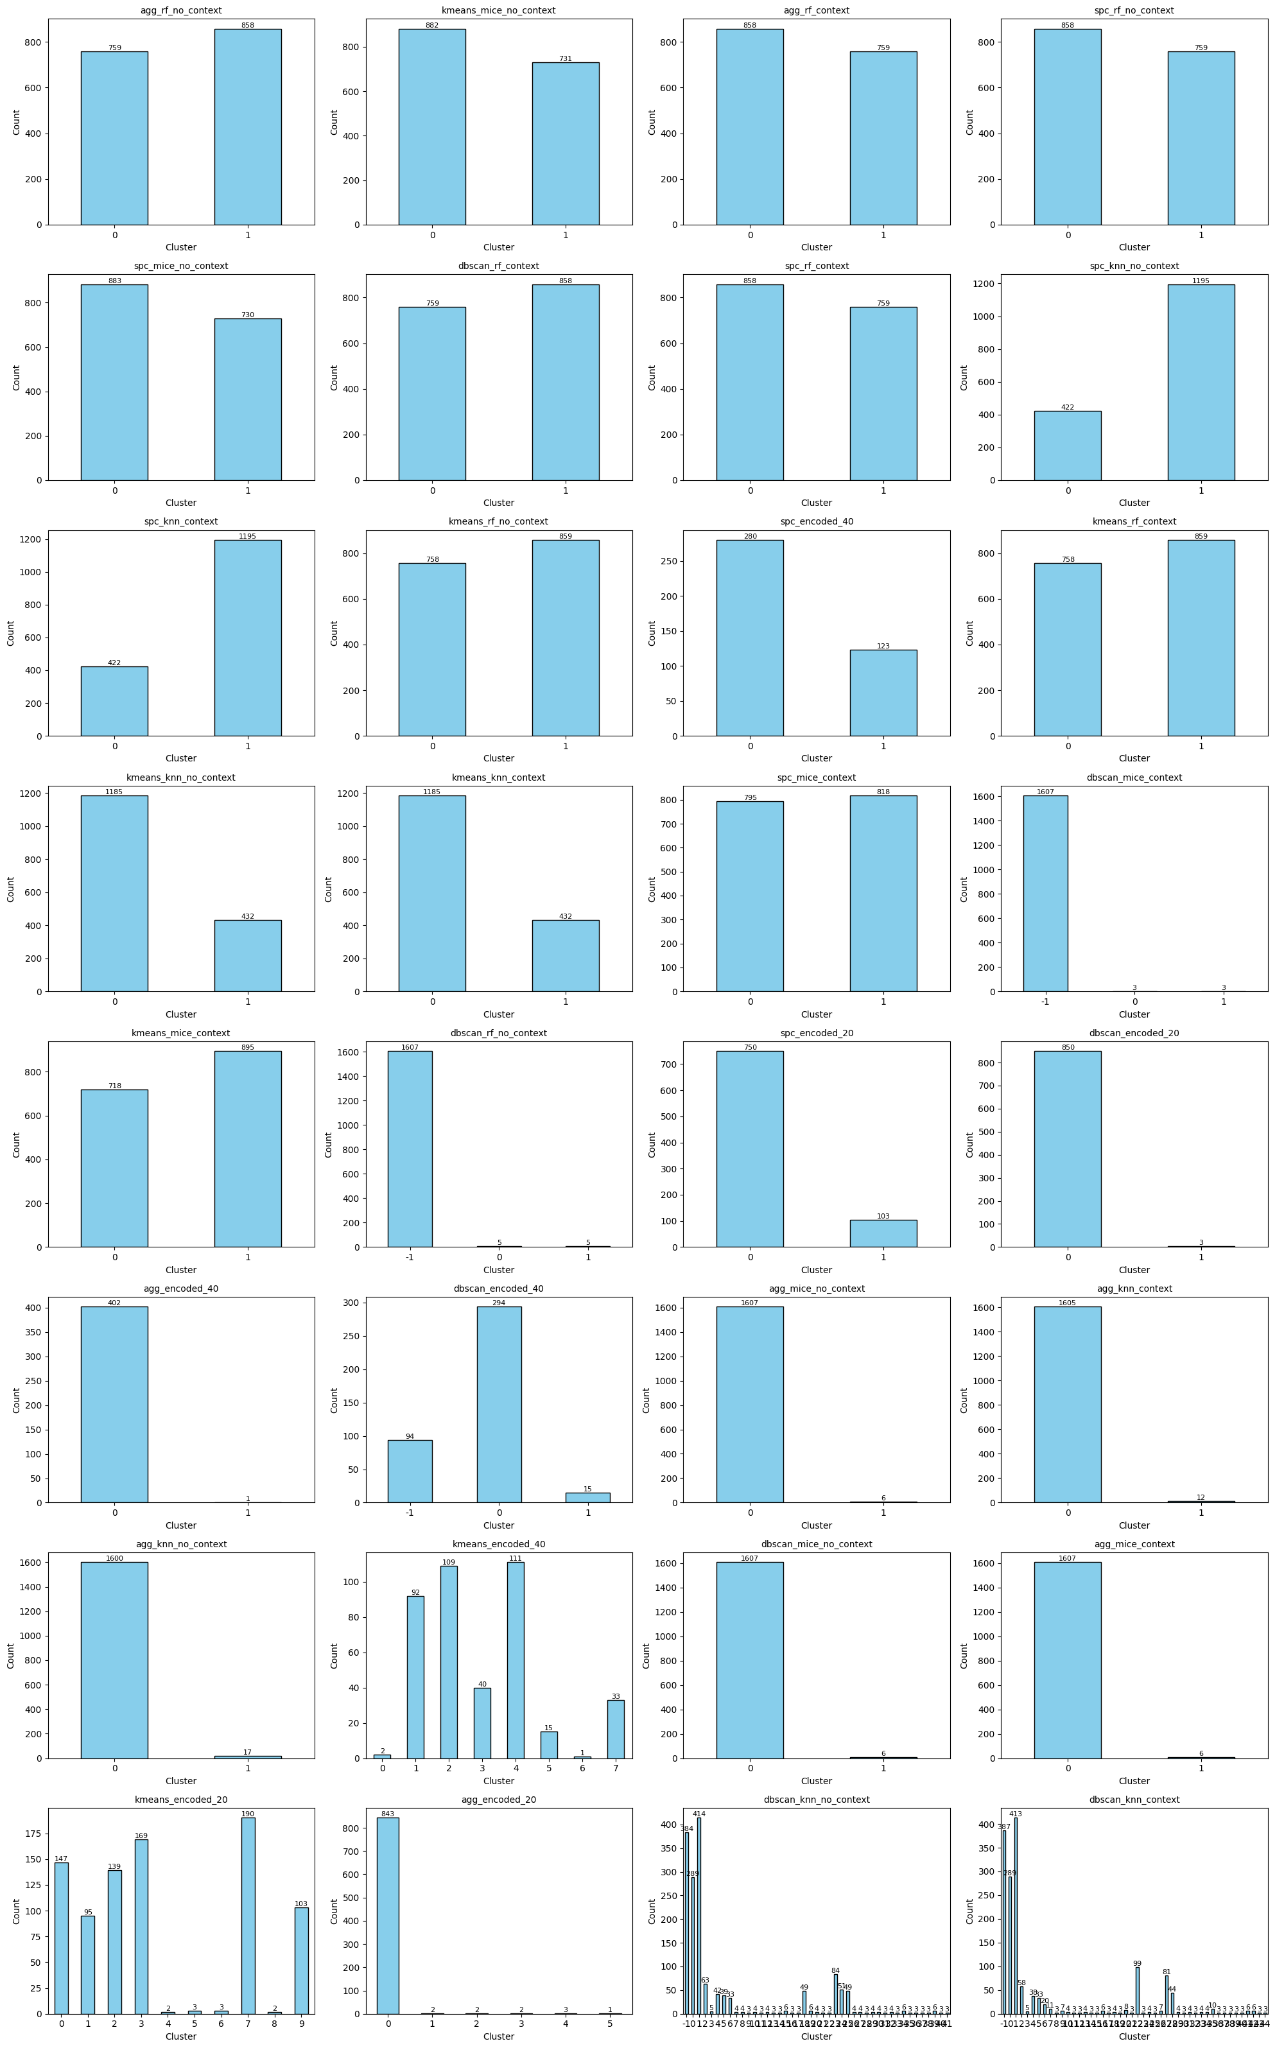
\includegraphics[width=\textwidth,height=0.9\textheight,keepaspectratio]{image8.png}
  \caption[PCA scatter grid for all 32 pipelines]{PCA-reduced scatter grid covering all 32 clustering pipelines (4 rows $\times$ 8 columns), sorted by descending composite rank. Points are coloured by their assigned cluster labels.}
  \label{fig:supplementary_figure_s2_full_p}
\end{figure}

\begin{figure}[!htb]
  \centering
  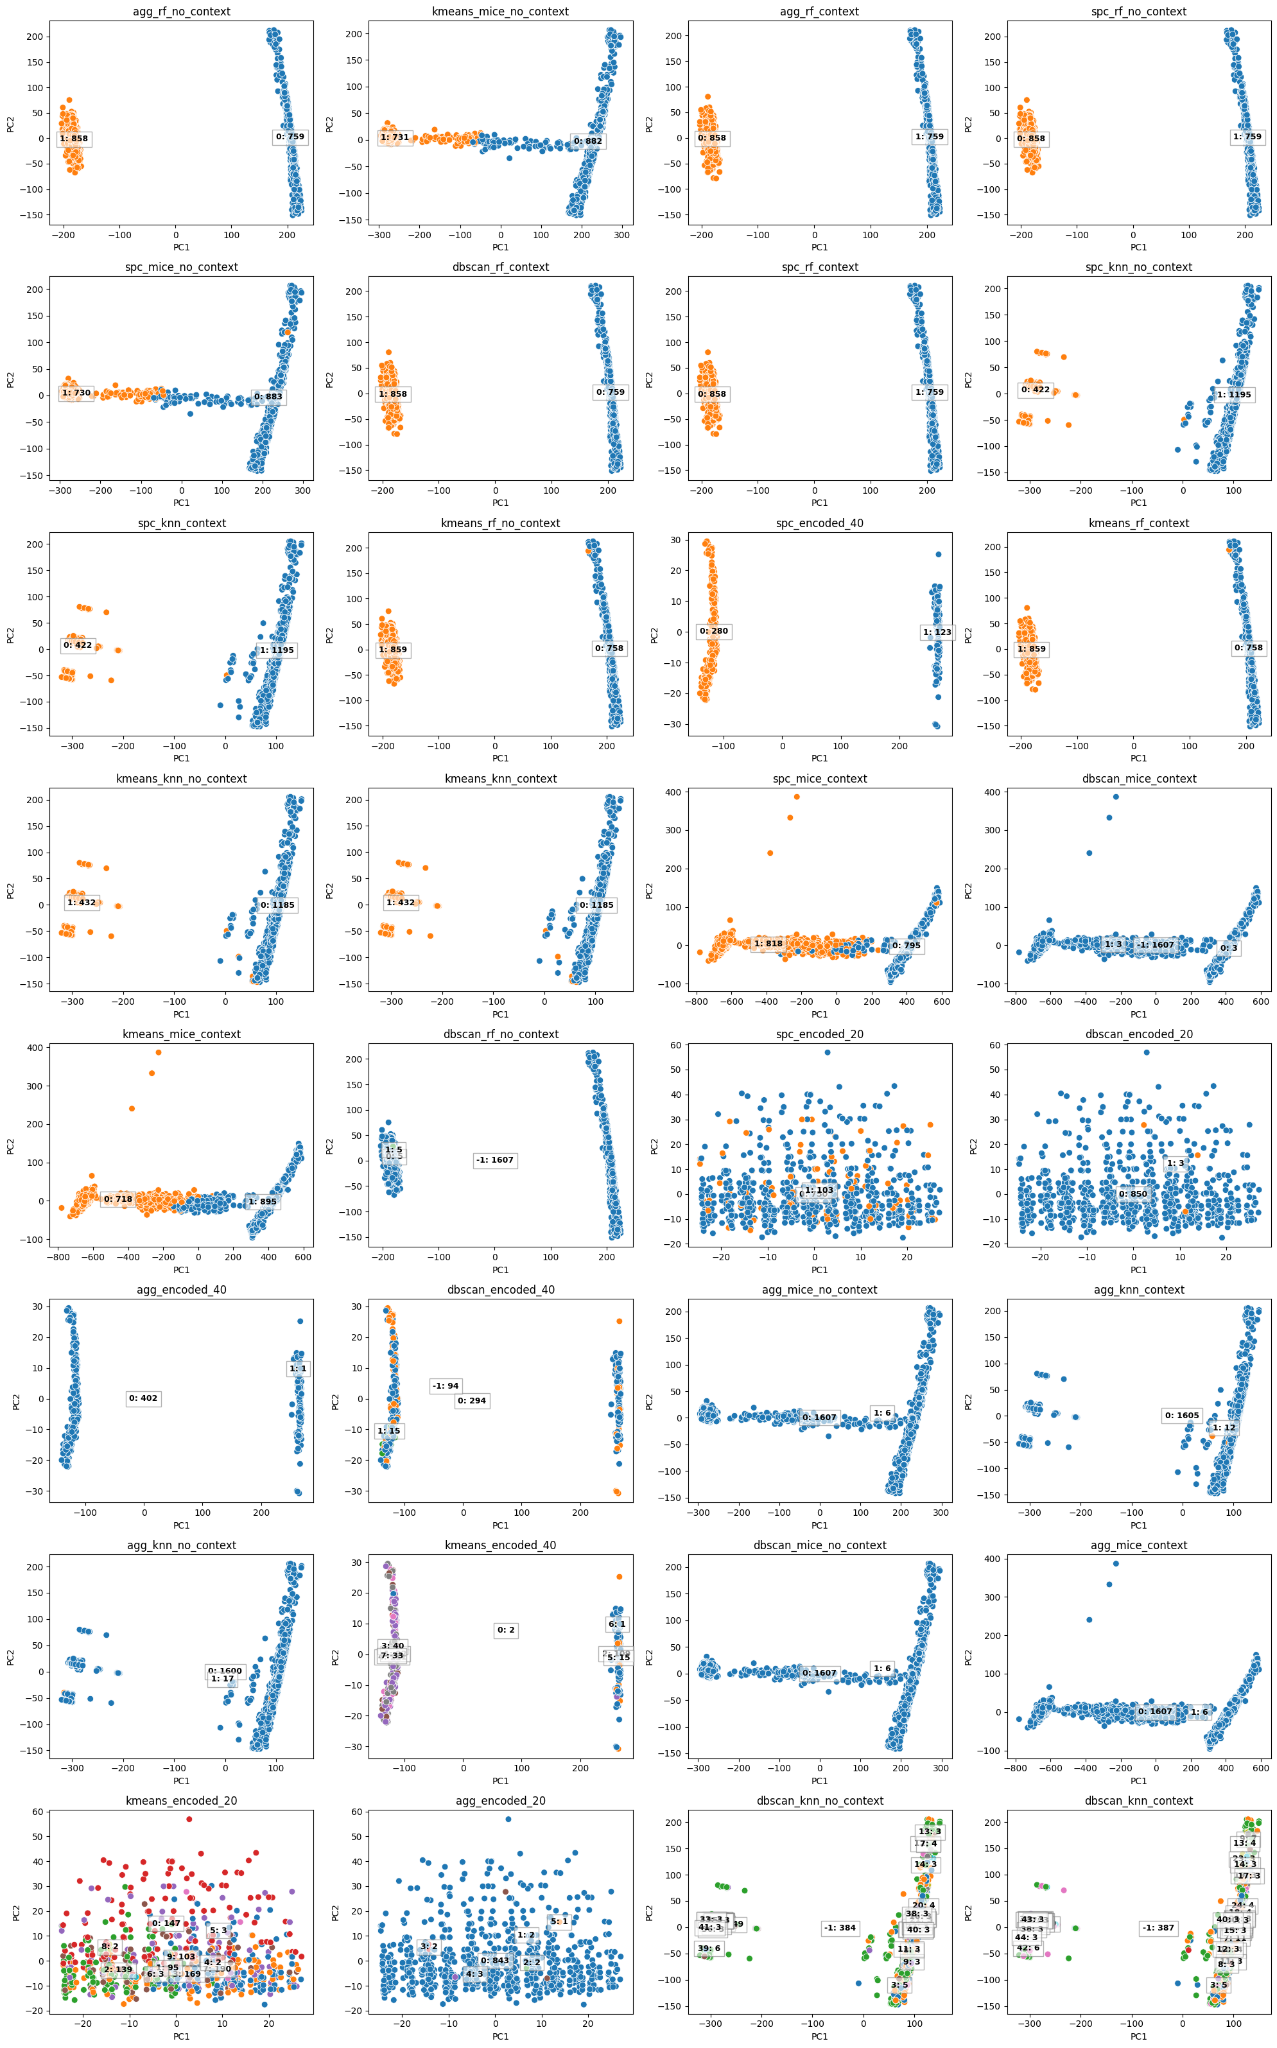
\includegraphics[width=\textwidth,height=0.9\textheight,keepaspectratio]{image14.png}
  \caption[Cluster count across all 32 pipelines]{Full bar graph of the number of unique clusters (excluding noise labels of $-1$ in DBSCAN) across all 32 pipelines.}
  \label{fig:supplementary_figure_s3_full_b}
\end{figure}

% Numerical comparison — the source PNG is too tall to fit one page at
% readable width, so it was pre-split into 4 vertical quarters
% (all_numerical_comparison_p1.png ... _p4.png). \ContinuedFloat keeps all
% four sub-figures under the same logical number (S3); the empty short-caption
% [] on parts 2–4 suppresses extra List-of-Figures entries.
\begin{figure}[H]
  \centering
  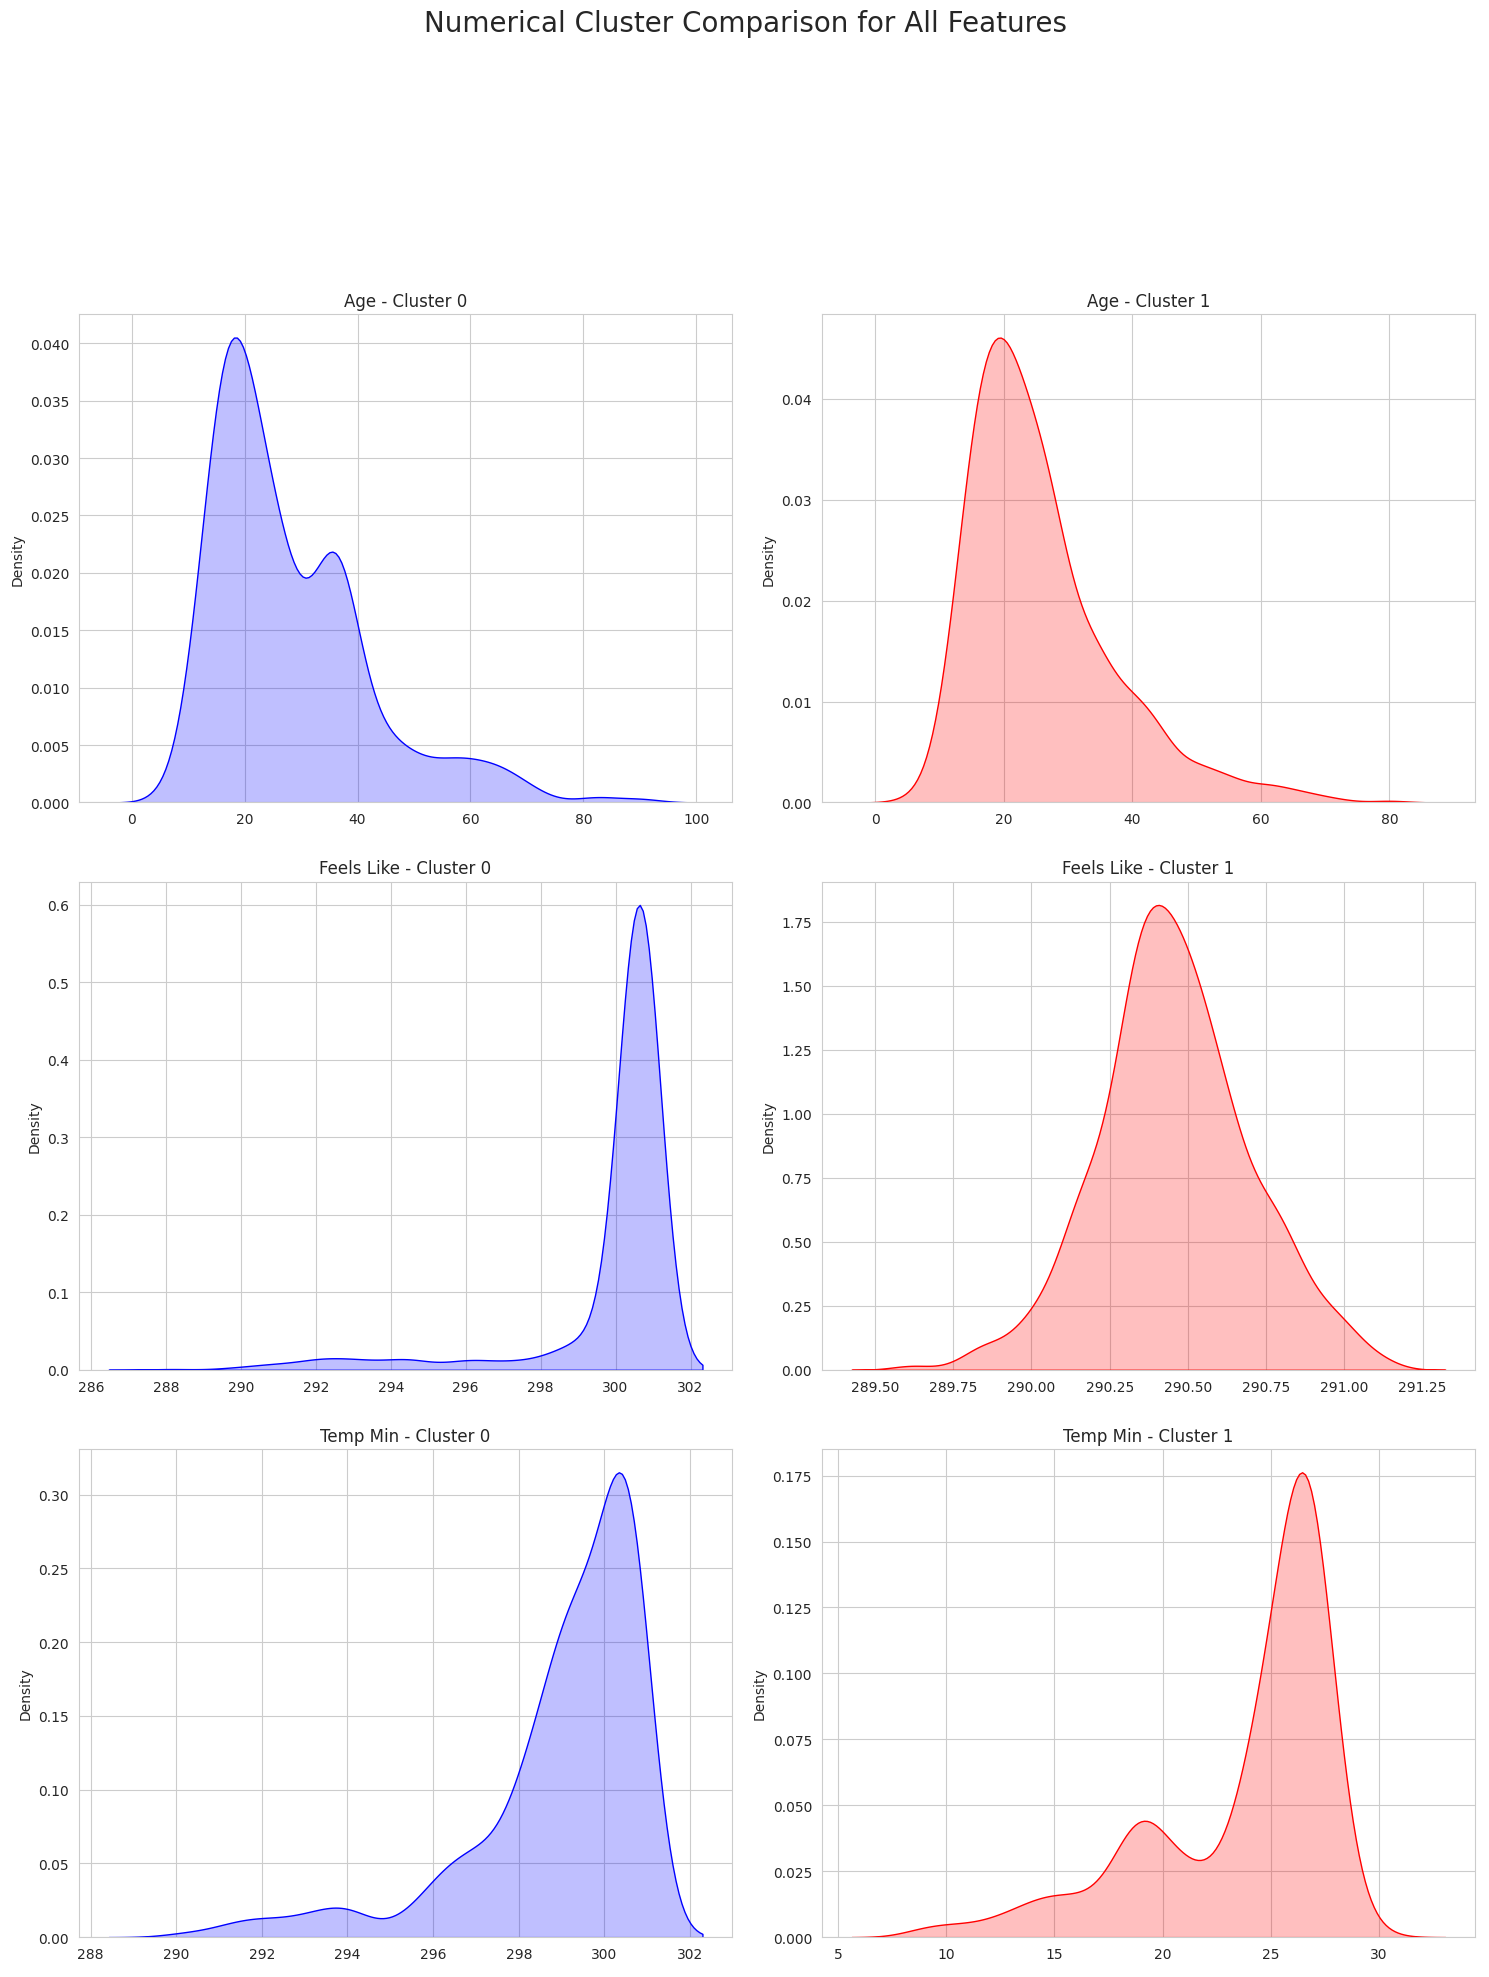
\includegraphics[width=\textwidth,height=0.9\textheight,keepaspectratio]{all_numerical_comparison_p1.png}
  \caption[Numerical feature distributions, best pipeline, part 1]{Cluster~0 (blue) versus Cluster~1 (red) density distributions for every numerical feature in the best-performing pipeline (\texttt{agg\_rf\_no\_context}). Part 1 of 4.}
  \label{fig:appendix_numerical_all}
\end{figure}

\begin{figure}[H]
  \ContinuedFloat
  \centering
  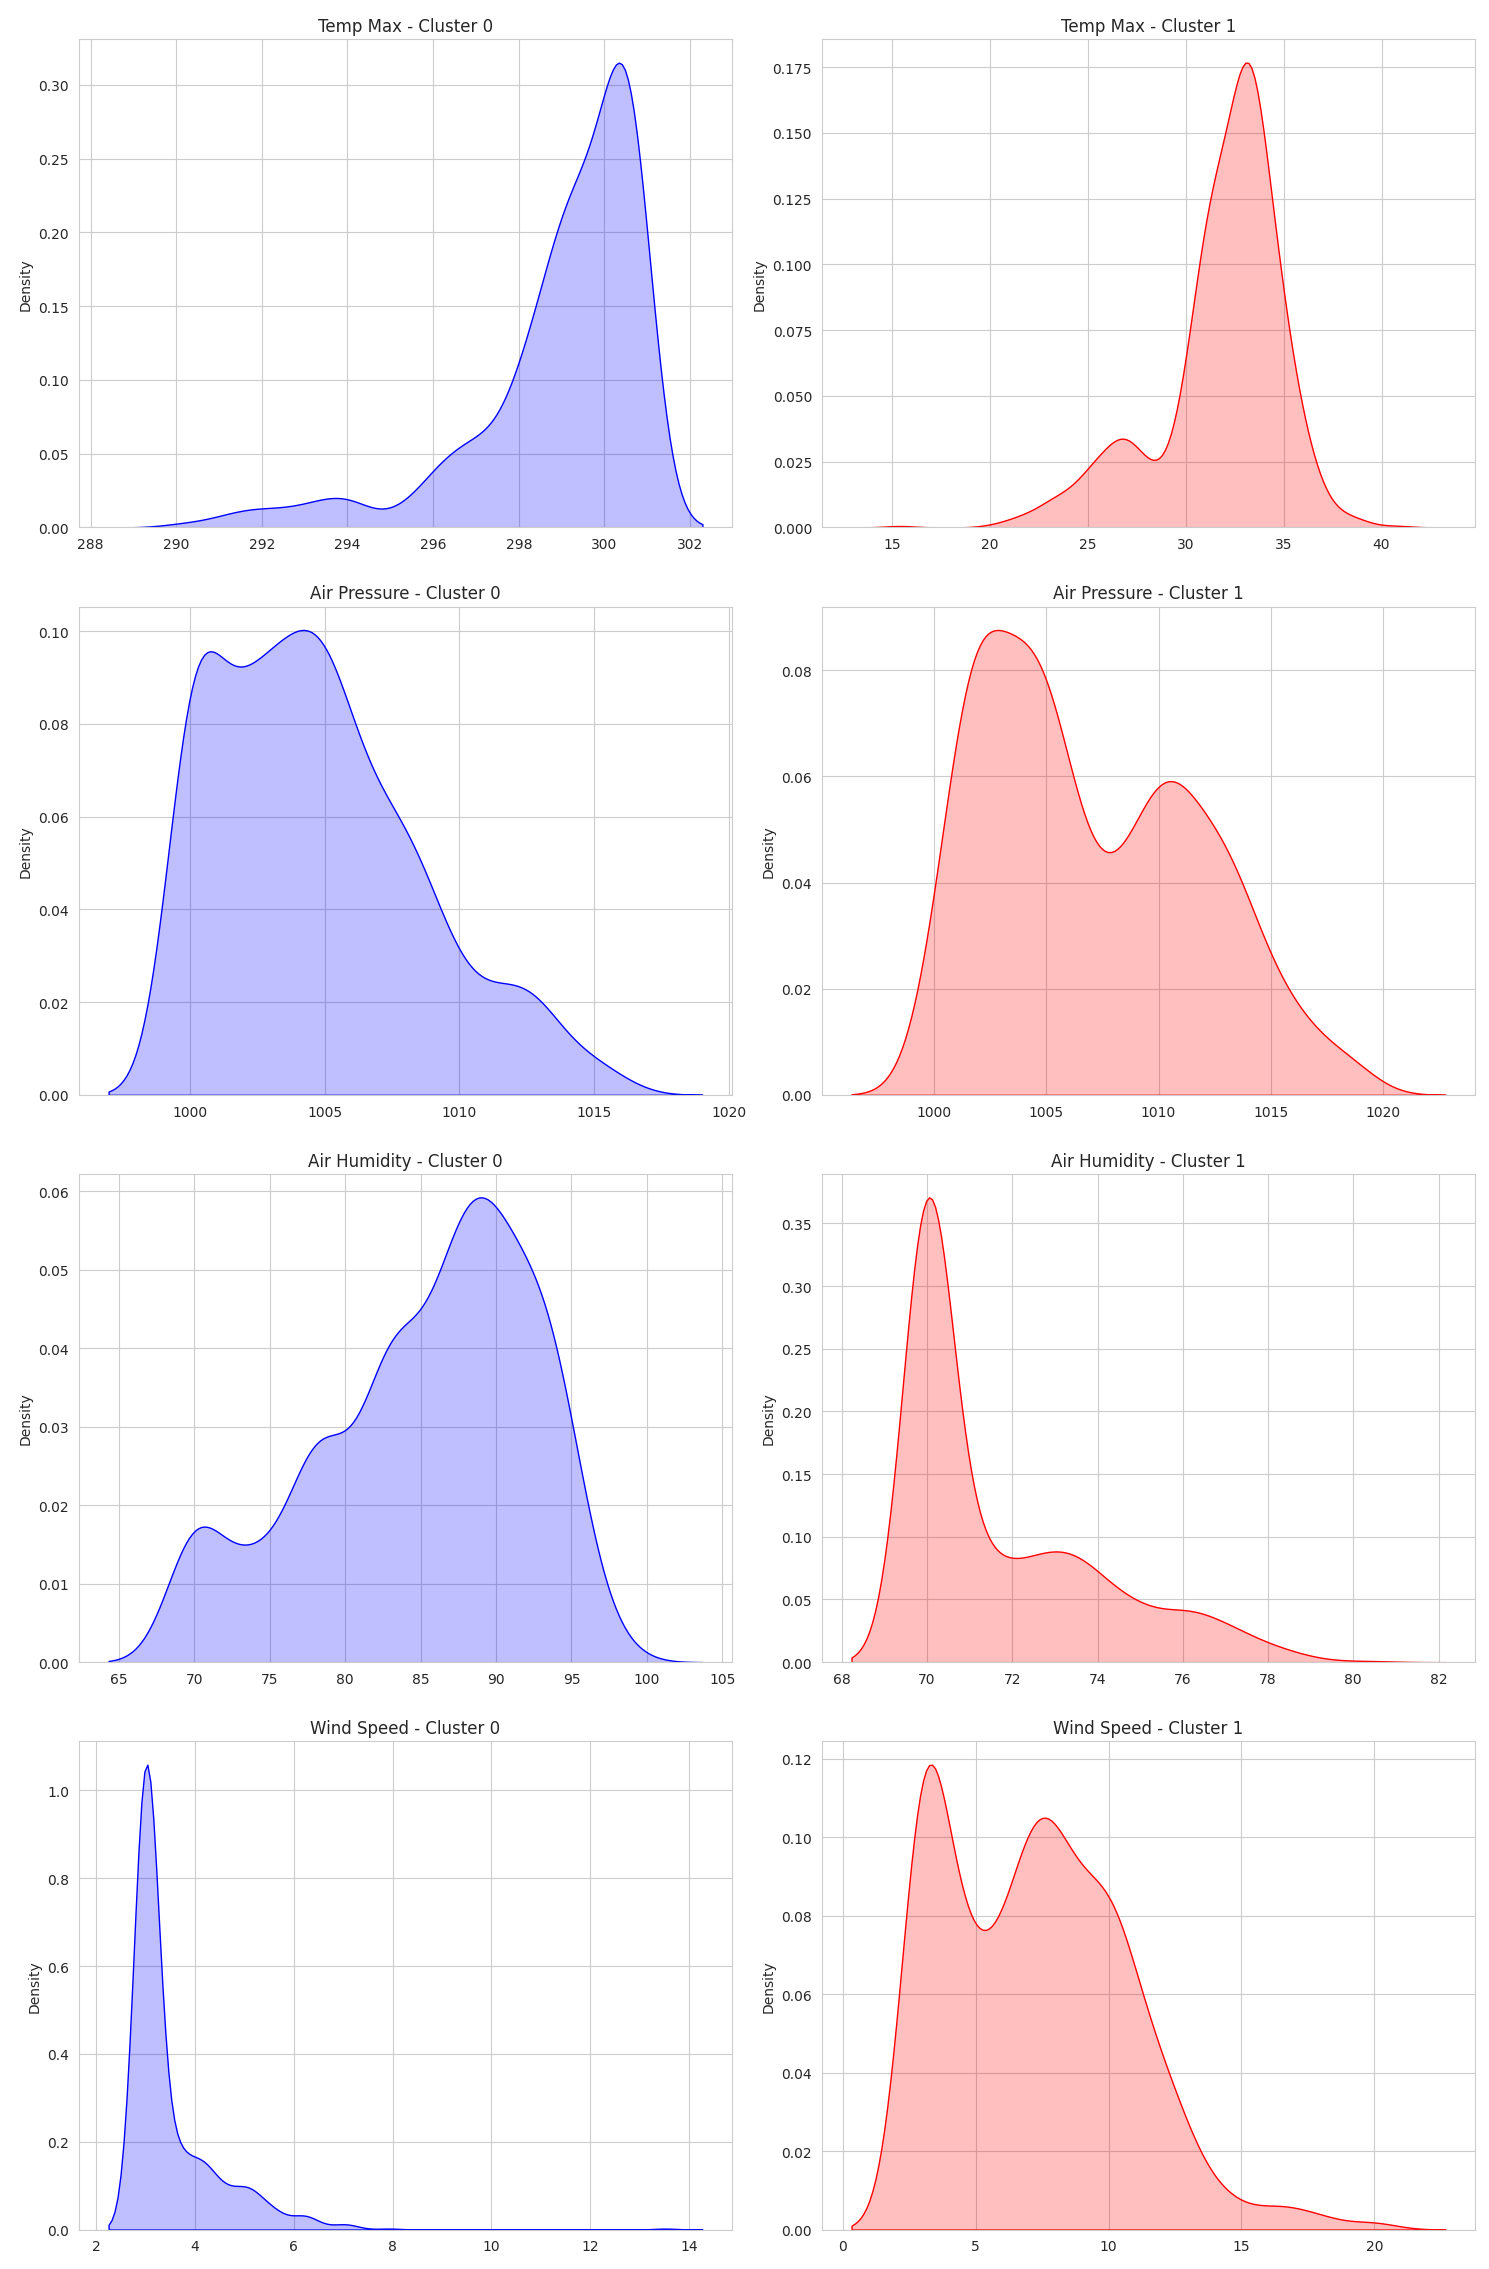
\includegraphics[width=\textwidth,height=0.9\textheight,keepaspectratio]{all_numerical_comparison_p2.png}
  \caption[]{Numerical feature comparison, part 2 of 4 (continued from Figure~\ref{fig:appendix_numerical_all}).}
\end{figure}

\begin{figure}[H]
  \ContinuedFloat
  \centering
  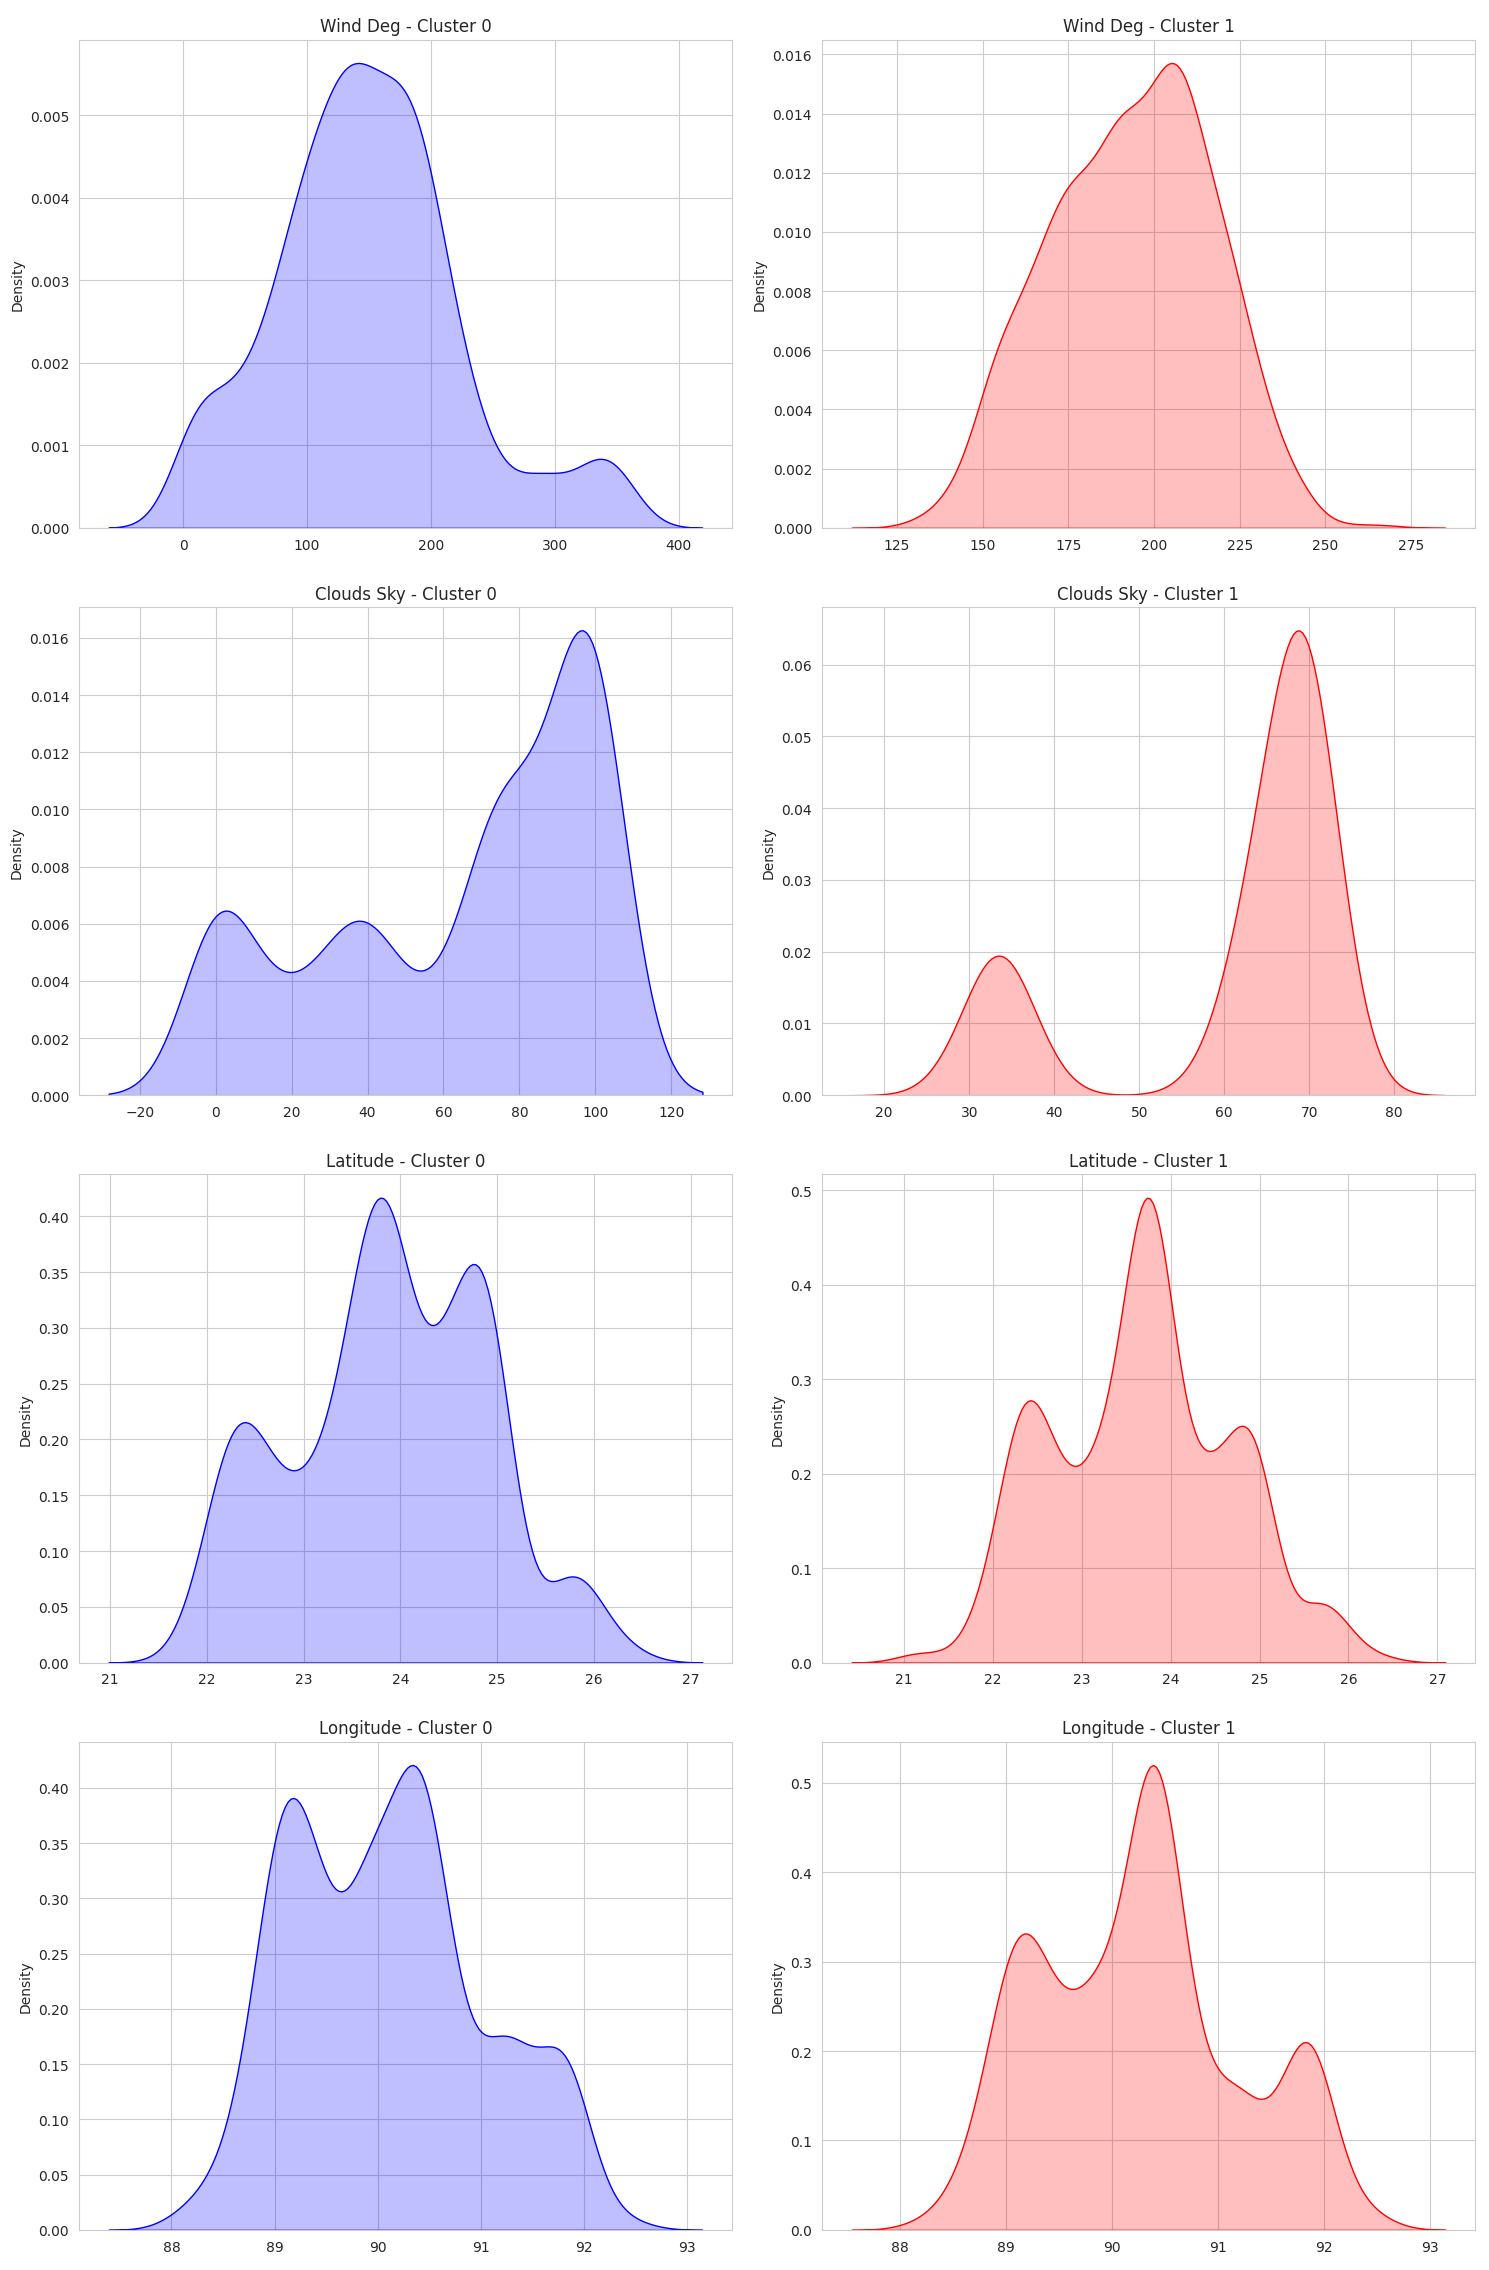
\includegraphics[width=\textwidth,height=0.9\textheight,keepaspectratio]{all_numerical_comparison_p3.png}
  \caption[]{Numerical feature comparison, part 3 of 4 (continued from Figure~\ref{fig:appendix_numerical_all}).}
\end{figure}

\begin{figure}[H]
  \ContinuedFloat
  \centering
  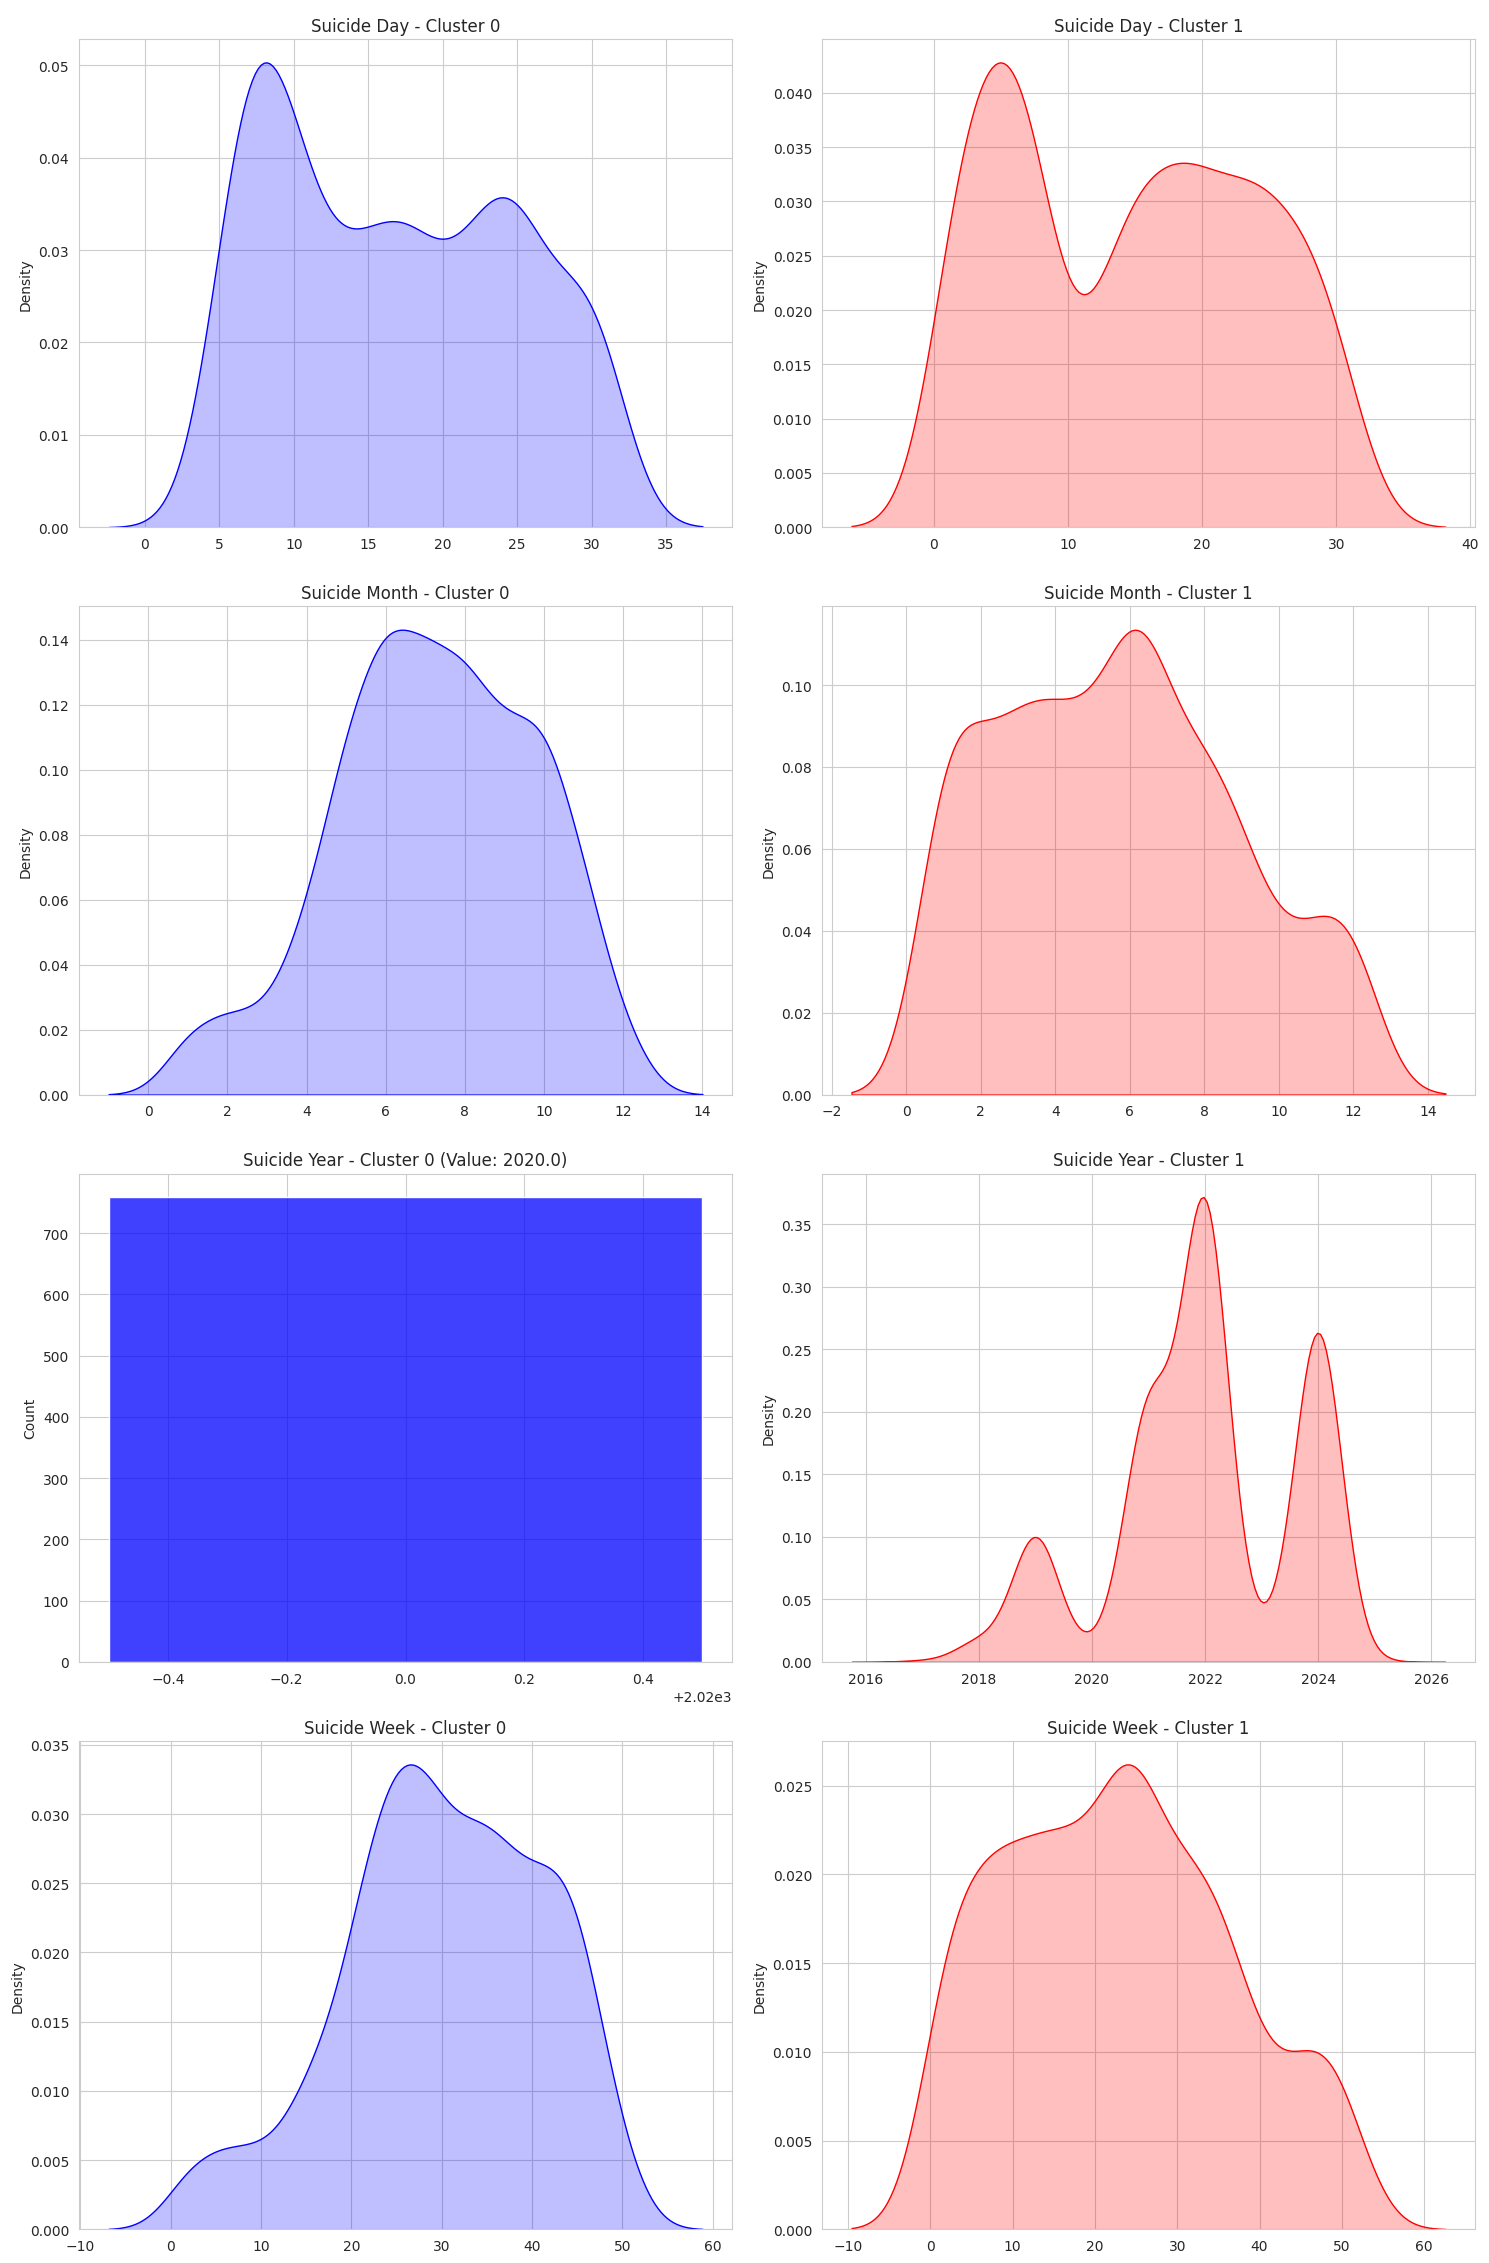
\includegraphics[width=\textwidth,height=0.9\textheight,keepaspectratio]{all_numerical_comparison_p4.png}
  \caption[]{Numerical feature comparison, part 4 of 4 (continued from Figure~\ref{fig:appendix_numerical_all}).}
\end{figure}

% Categorical comparison — same 4-part split approach.
\begin{figure}[H]
  \centering
  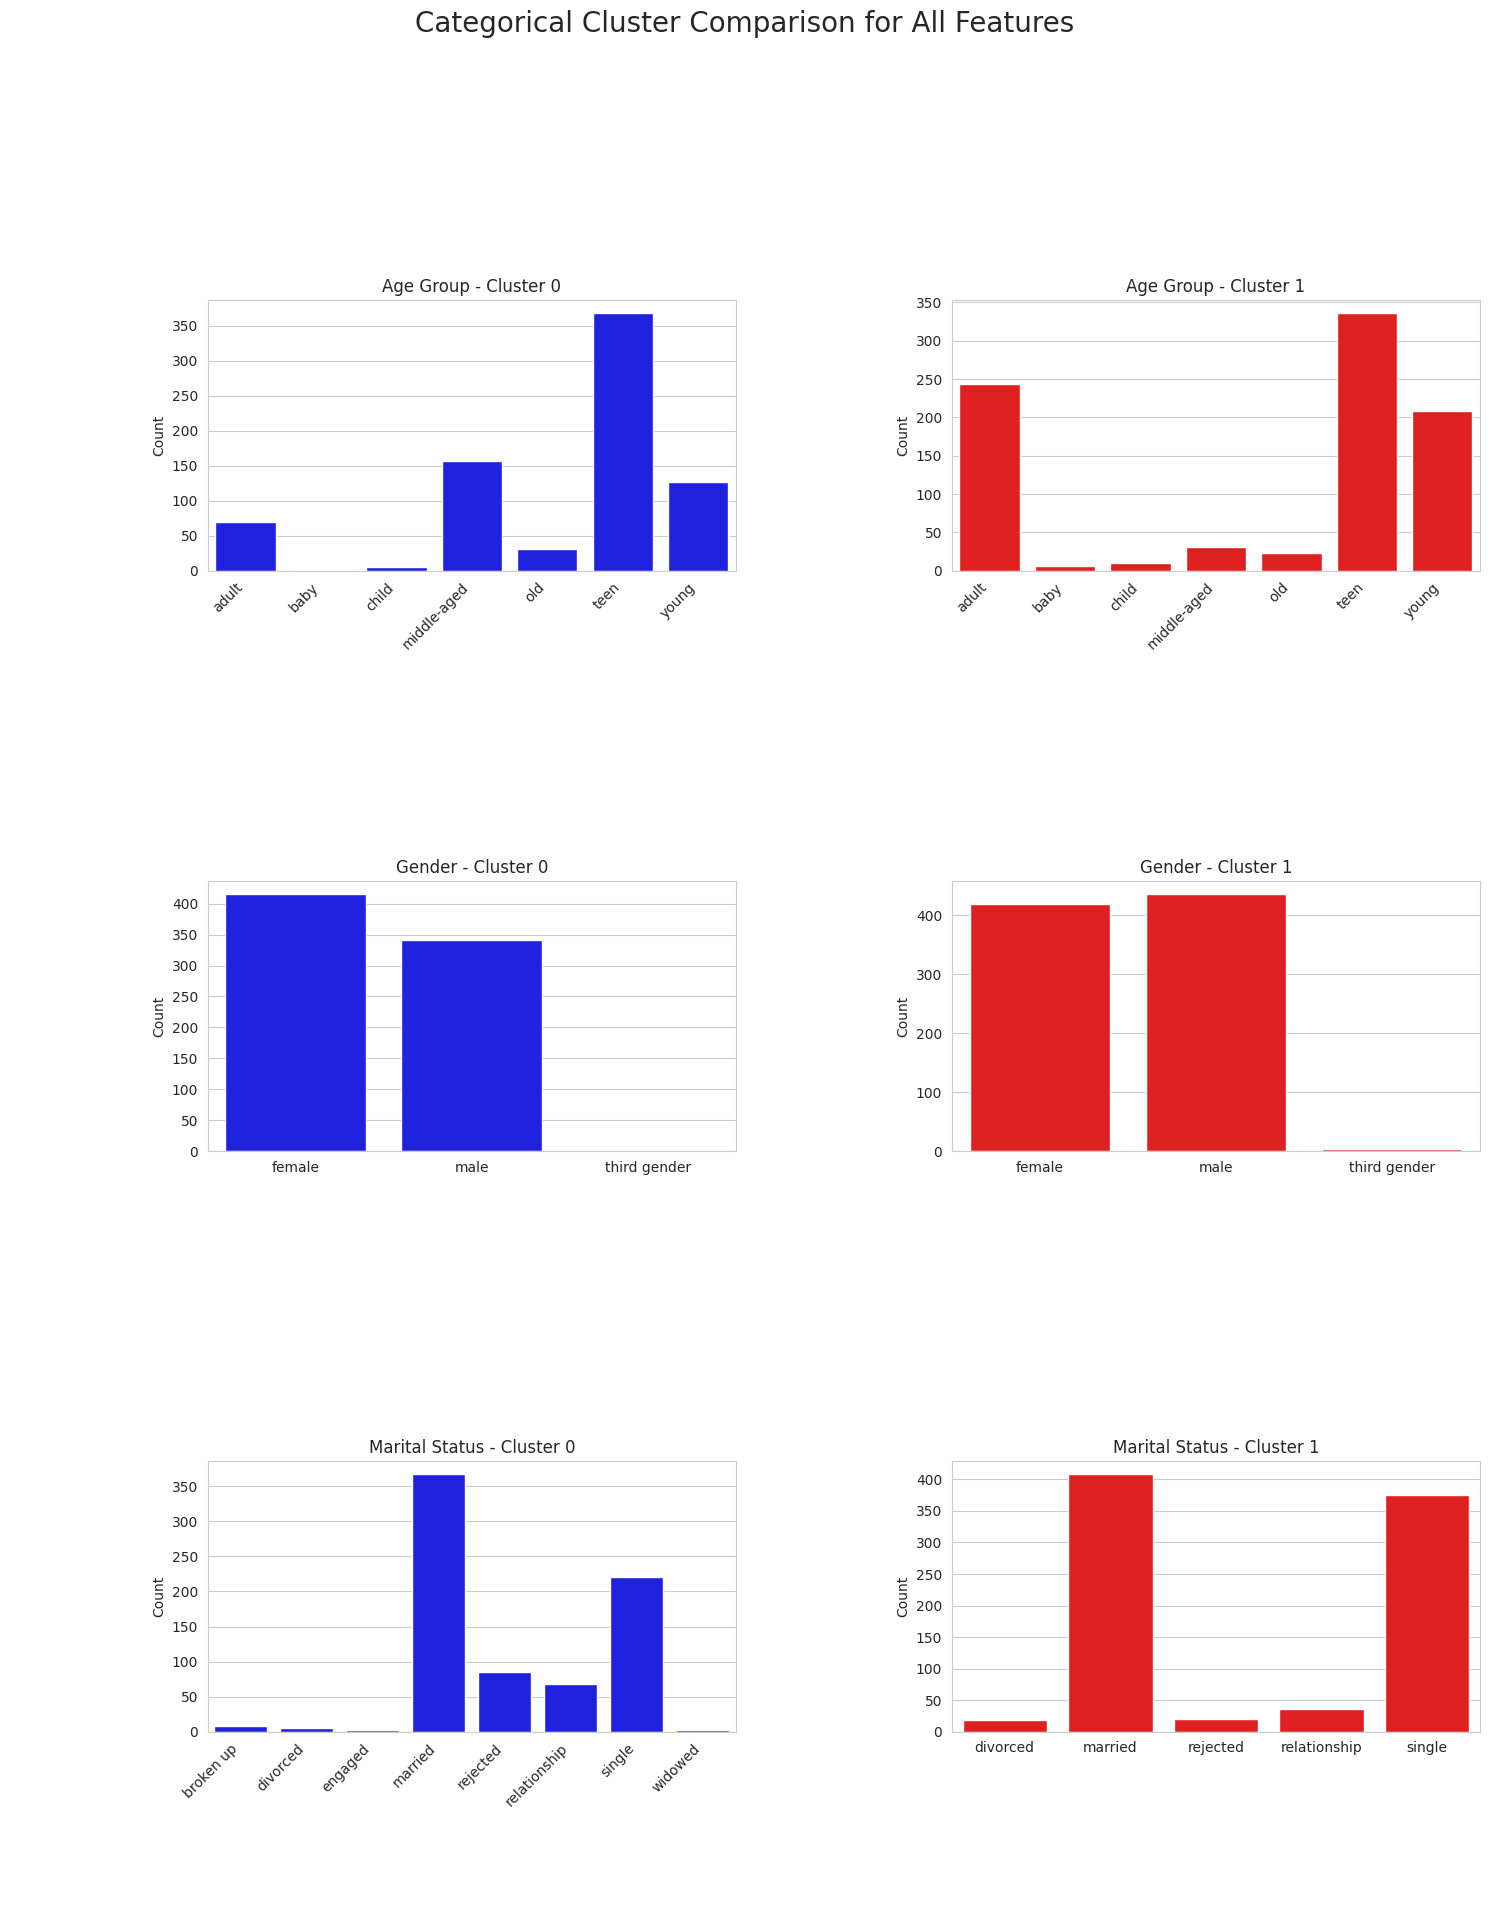
\includegraphics[width=\textwidth,height=0.9\textheight,keepaspectratio]{all_categoricaL_comparsion_p1.png}
  \caption[Categorical feature distributions, best pipeline, part 1]{Cluster~0 (blue) versus Cluster~1 (red) category-frequency bar charts for every categorical feature in the best-performing pipeline (\texttt{agg\_rf\_no\_context}). Part 1 of 4.}
  \label{fig:appendix_categorical_all}
\end{figure}

\begin{figure}[H]
  \ContinuedFloat
  \centering
  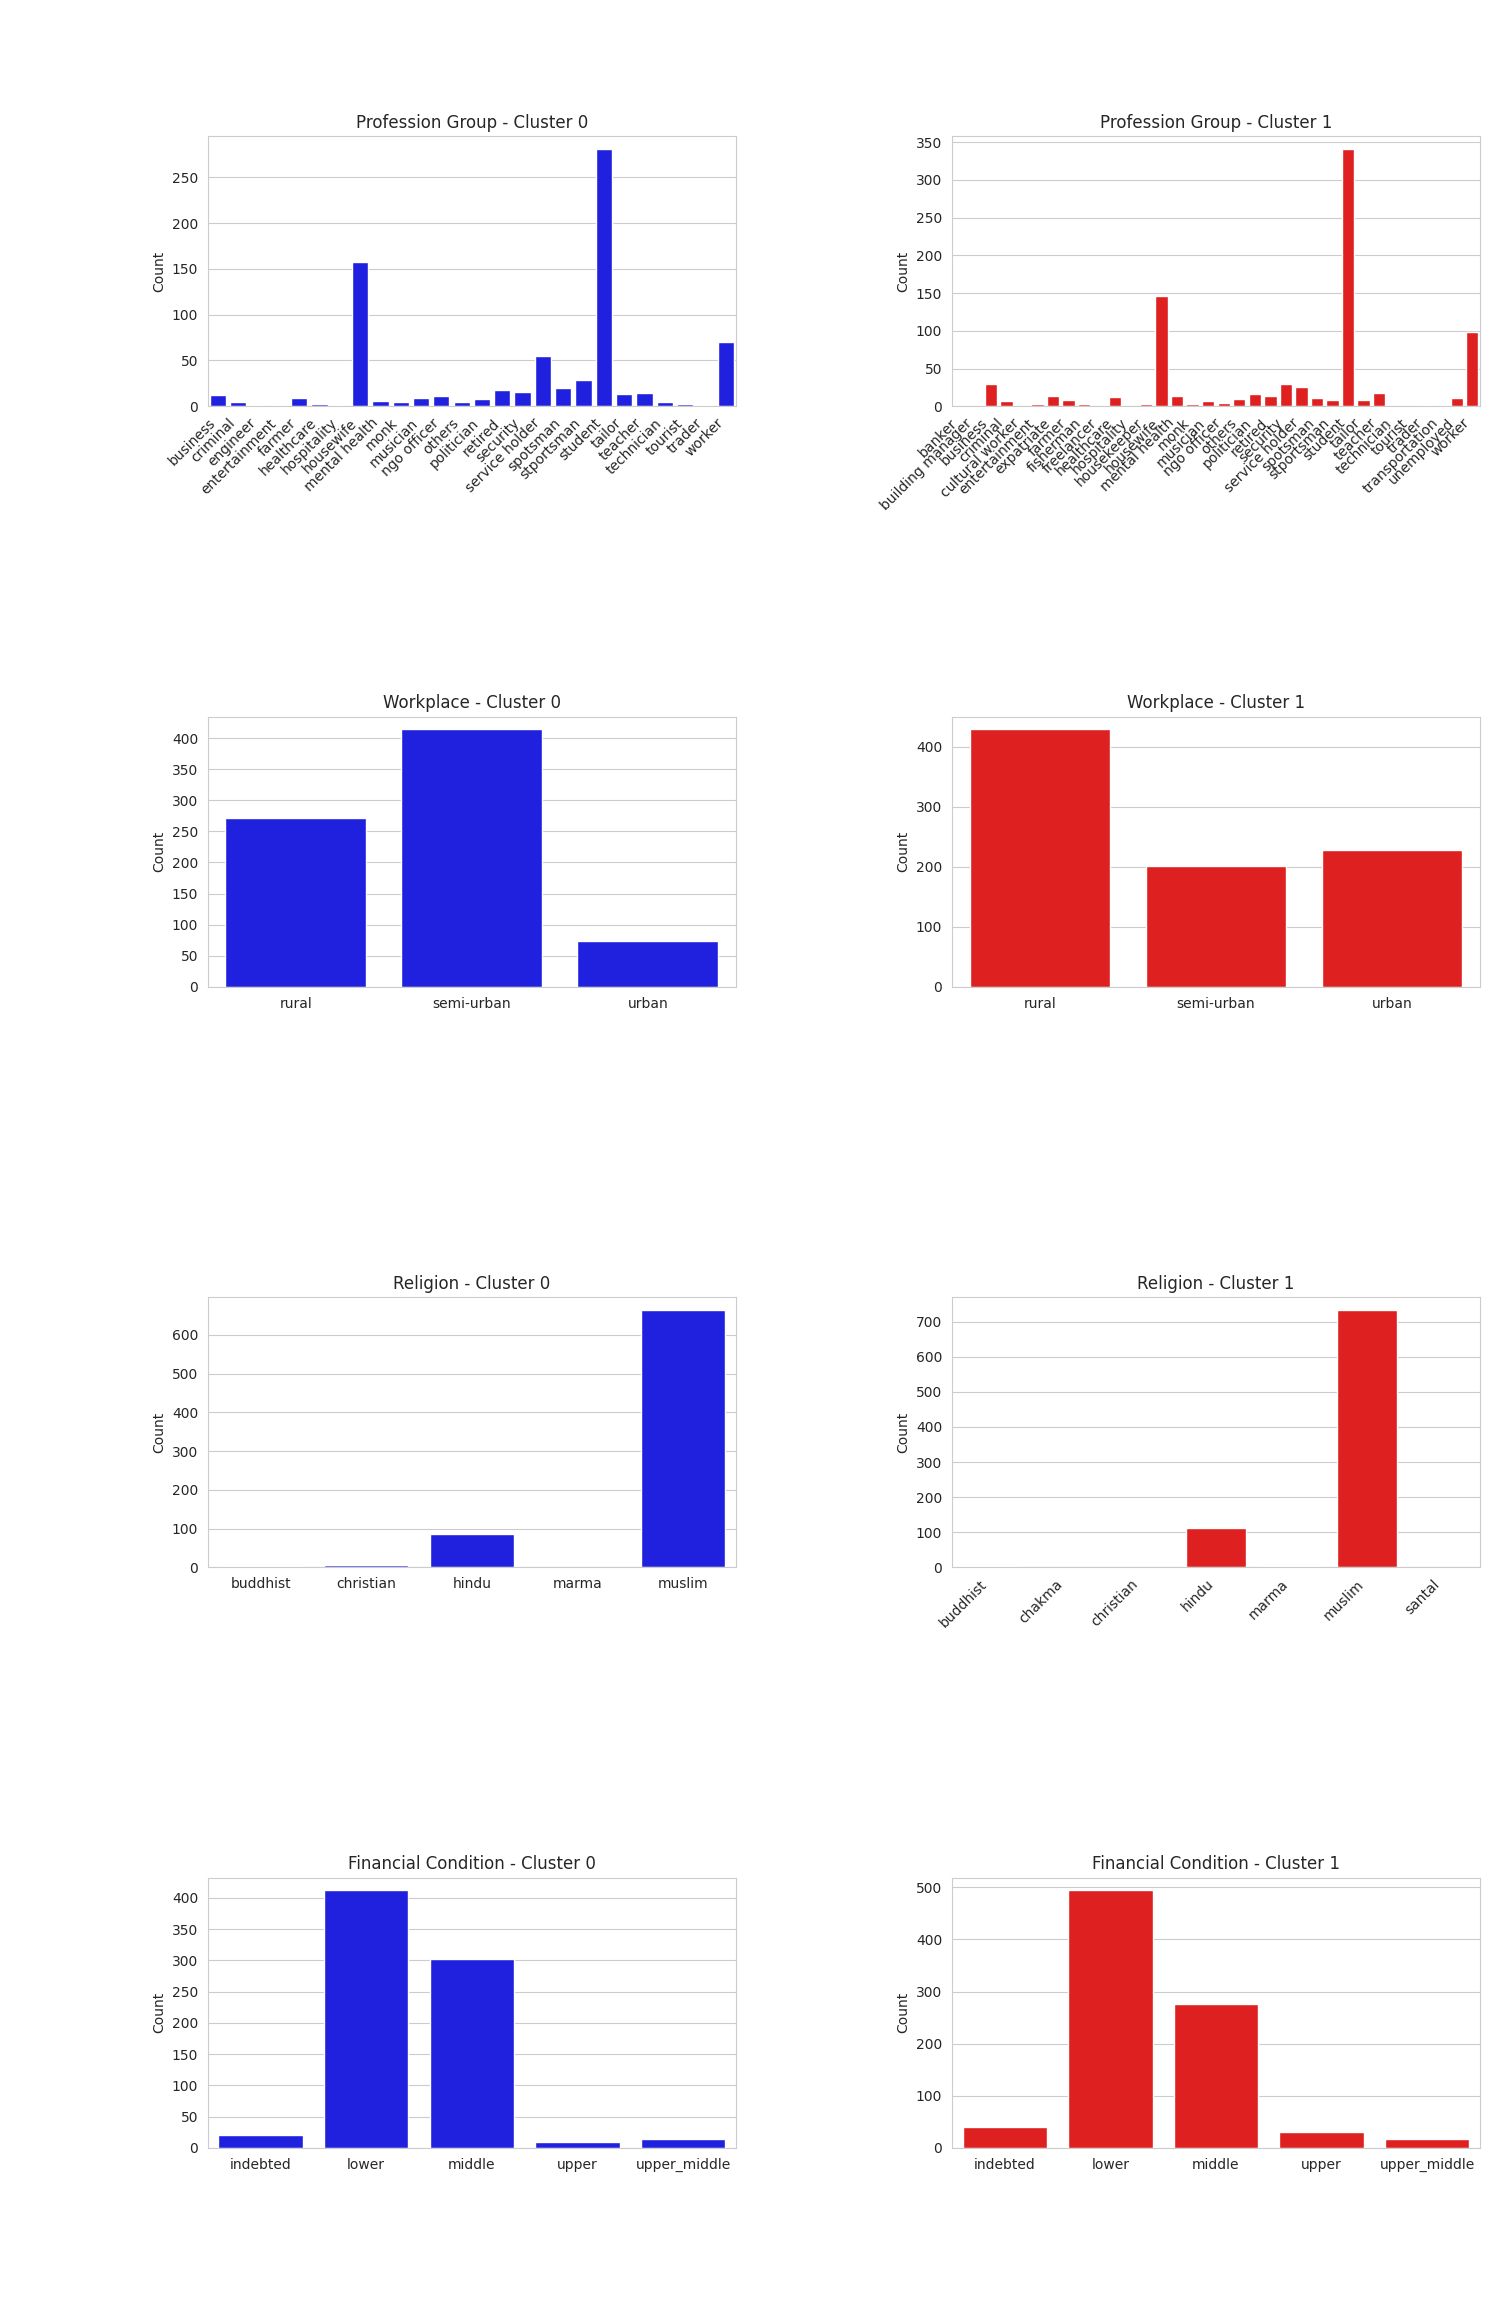
\includegraphics[width=\textwidth,height=0.9\textheight,keepaspectratio]{all_categoricaL_comparsion_p2.png}
  \caption[]{Categorical feature comparison, part 2 of 4 (continued from Figure~\ref{fig:appendix_categorical_all}).}
\end{figure}

\begin{figure}[H]
  \ContinuedFloat
  \centering
  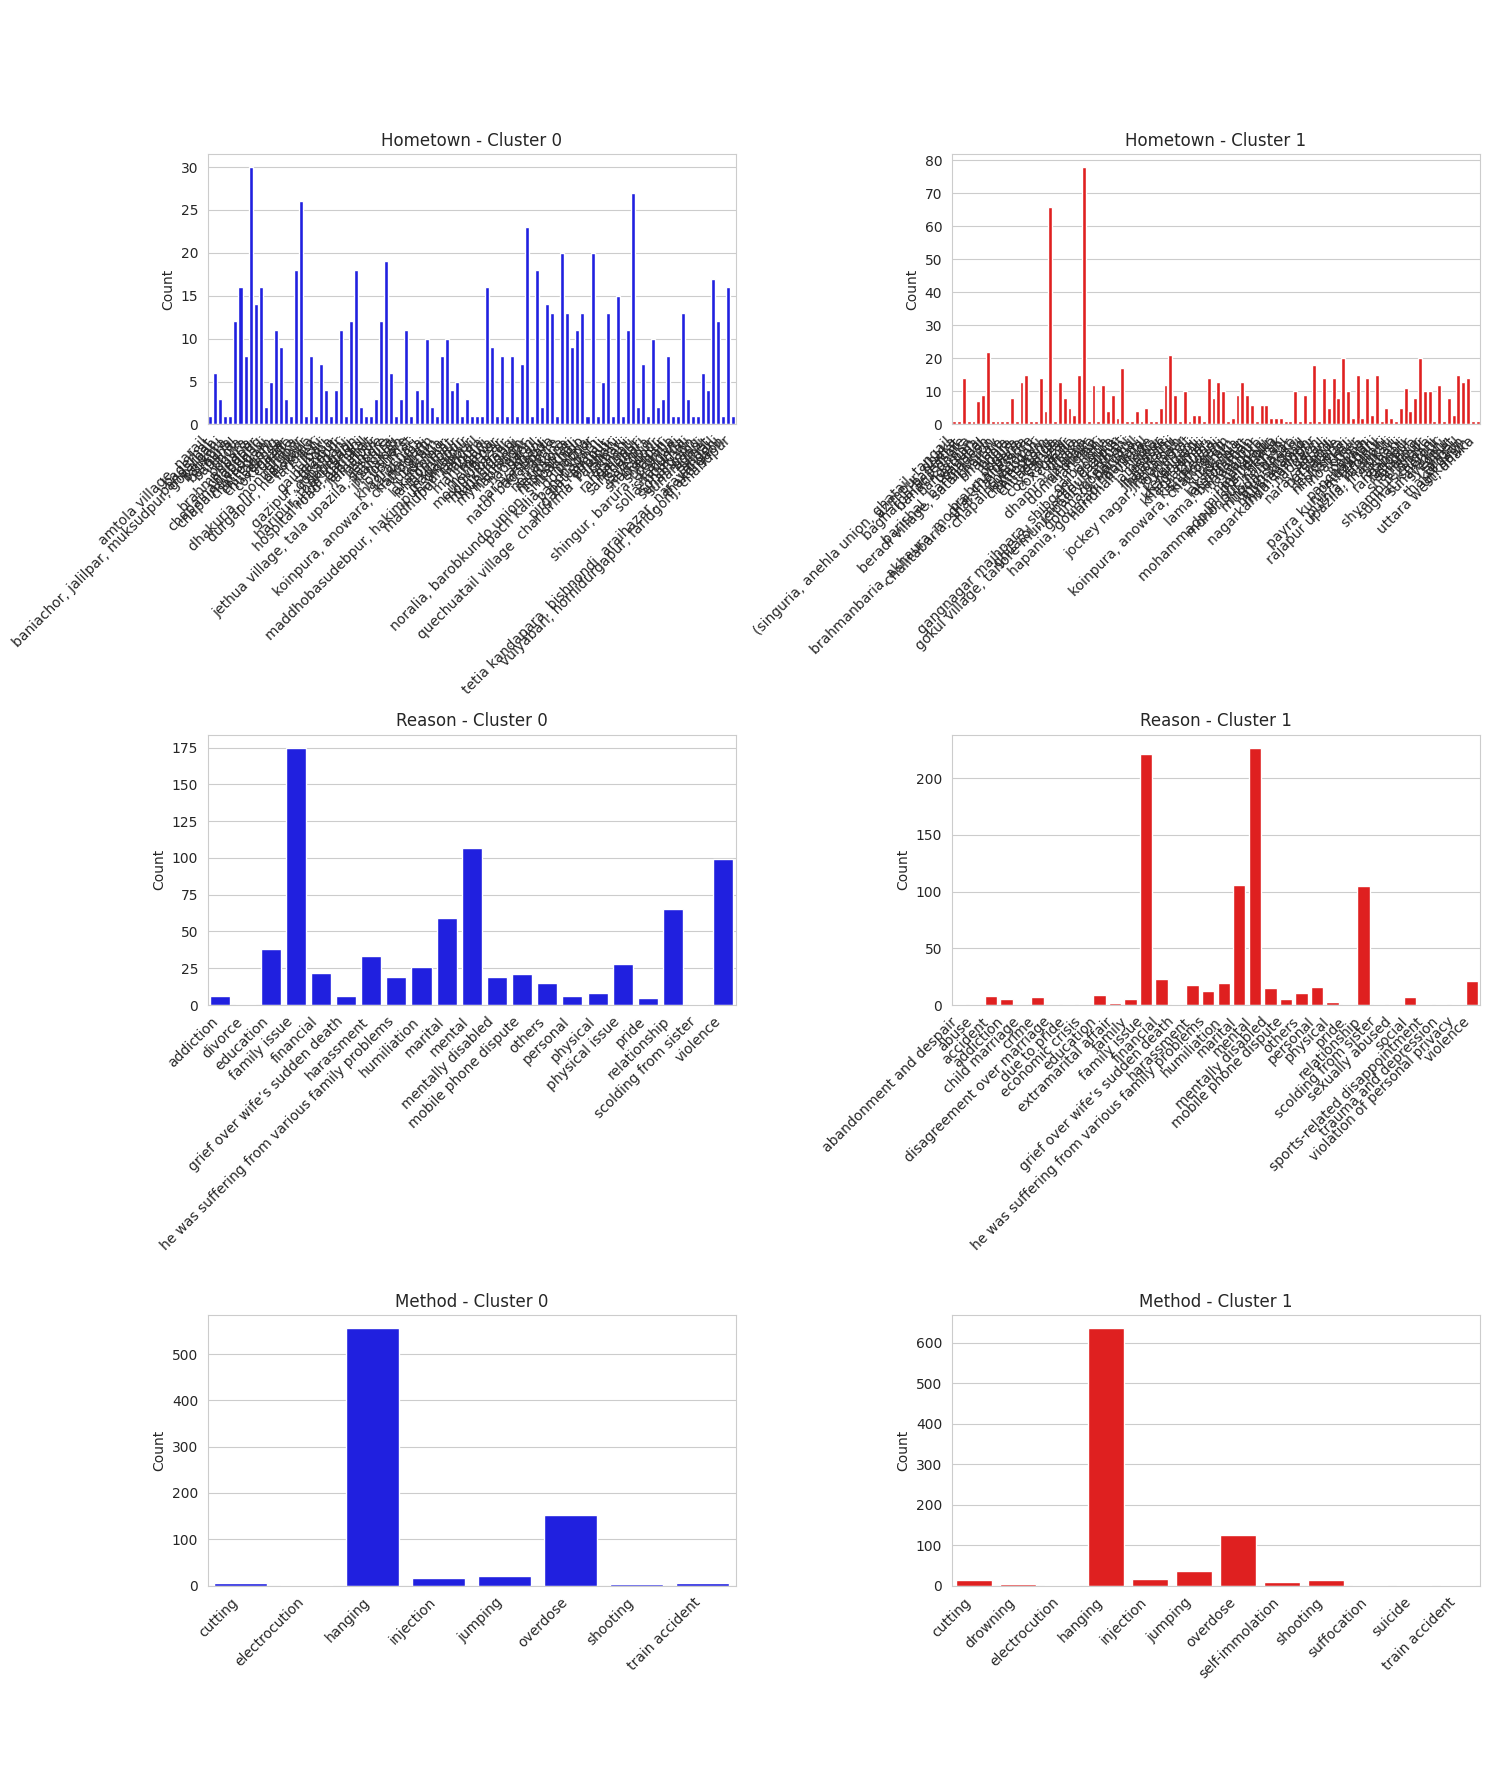
\includegraphics[width=\textwidth,height=0.9\textheight,keepaspectratio]{all_categoricaL_comparsion_p3.png}
  \caption[]{Categorical feature comparison, part 3 of 4 (continued from Figure~\ref{fig:appendix_categorical_all}).}
\end{figure}

\begin{figure}[H]
  \ContinuedFloat
  \centering
  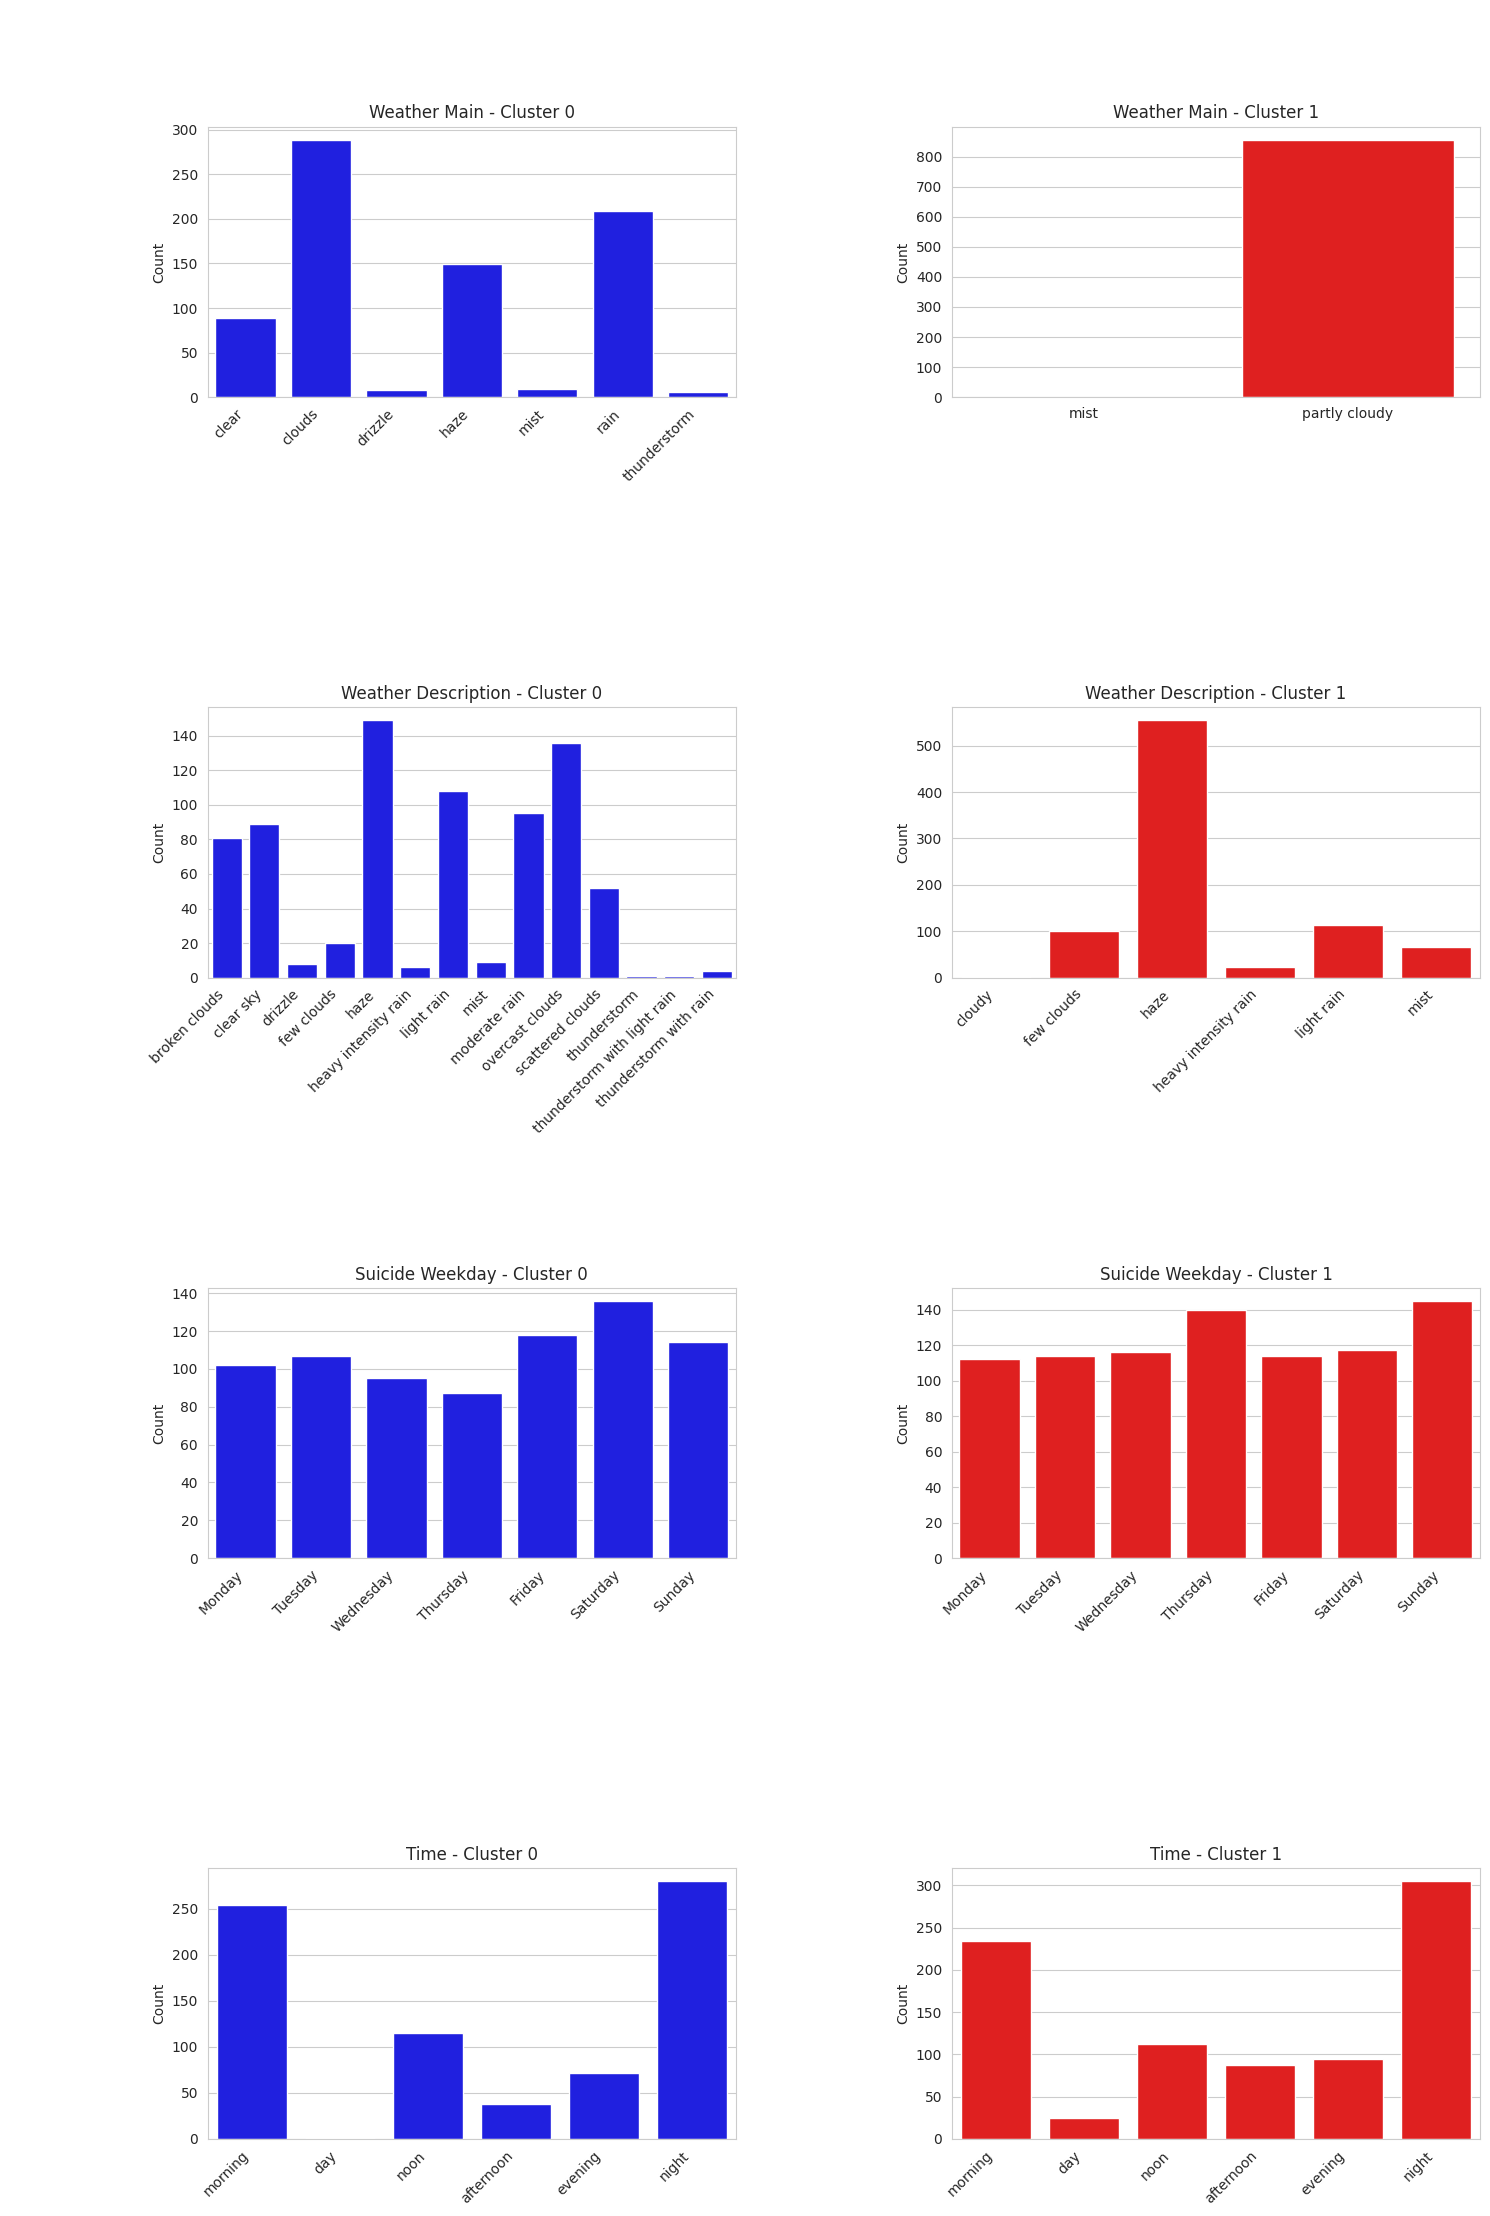
\includegraphics[width=\textwidth,height=0.9\textheight,keepaspectratio]{all_categoricaL_comparsion_p4.png}
  \caption[]{Categorical feature comparison, part 4 of 4 (continued from Figure~\ref{fig:appendix_categorical_all}).}
\end{figure}



\end{document}
